\section[Group -- Internal Gains]{Group -- Internal Gains (People, Lights, Other internal zone equipment)\sectionmark{Group -- Internal Gains}}\label{group-internal-gains-people-lights-other-internal-zone-equipment}
\sectionmark{Group -- Internal Gains}

Not all the influence for energy consumption in the building is due to envelope and ambient conditions. This group of objects describes other internal gains that may come into play (\hyperref[people]{People}, \hyperref[lights-000]{Lights}, Various Equipment Types).

\subsection{People}\label{people}

The people statement is used to model the occupant's effect on the space conditions. The following definition addresses the basic affects as well as providing information that can be used to report the thermal comfort of a group of occupants. The Fanger, Pierce Two-Node, Kansas State University Two-Node, ASHRAE Standard 55 Elevated Air Cooling Effect model, and ASHRAE Standard 55 Ankle Draft Risk thermal comfort models are available in EnergyPlus. A user may select any of these models for each People statement by simply adding the appropriate choice keyword after the air velocity schedule name. Thermal comfort calculations will only be made for people statements that include specific requests for these thermal comfort models. This object also requires input of carbon dioxide generation rate based on people activity level for zone carbon dioxide simulations.

\subsubsection{Inputs}\label{inputs-025}

\paragraph{Field: Name}\label{field-name-024}

The name of the People object. Must be unique across all People objects.

\paragraph{Field: Zone or ZoneList Name}\label{field-zone-or-zonelist-name-000}

This field is the name of the zone (ref: Zone) or \hyperref[zonelist]{ZoneList} (ref: \hyperref[zonelist]{ZoneList}) and links a particular people statement to a thermal zone or set of thermal zones in the building. When the \hyperref[zonelist]{ZoneList} option is used then this people definition is applied to each of the zones in the zone list effecting a global definition for the number of people in the zone. The Zonelist option can be used effectively with the people/area and area/person options of the Number of People Calculation Method.

The name of the actual people object becomes \textless{}Zone Name\textgreater{} \textless{}People Object Name\textgreater{} and should be less than the standard length (100 characters) for a name field. If it is greater than this standard length, it may be difficult to specify in output reporting as it will be truncated. A warning will be shown if the generated name is greater than 100 characters. If it duplicates another such concatenated name, there will be a severe error and terminate the run.

\paragraph{Field: Number of People Schedule Name}\label{field-number-of-people-schedule-name}

This field is the name of the schedule (ref: Schedules) that modifies the number of people parameter (see Number of People Calculation Method and related fields). The schedule values can be any positive number. The actual number of people in a zone as defined by this statement is the product of the number of people field and the value of the schedule specified by name in this field.

\paragraph{Field: Number of People Calculation Method}\label{field-number-of-people-calculation-method}

This field is a key/choice field that tells which of the next three fields are filled and is descriptive of the method for calculating the nominal number of occupants (people) in the Zone. The key/choices are:

\begin{itemize}
\tightlist
\item
  People
\end{itemize}

With this choice, the method used will be a straight insertion of the number of occupants (people).~ (The Number of People field should be filled.)

\begin{itemize}
\tightlist
\item
  People/Area
\end{itemize}

With this choice, the method used will be a factor per floor area of the zone. (The People per Zone Floor Area field should be filled).

\begin{itemize}
\tightlist
\item
  Area/Person
\end{itemize}

With this choice, the method used will be a factor of floor area per person. (The Zone Floor Area per Person field should be filled).

\paragraph{Field: Number of People}\label{field-number-of-people}

This field is used to represent the maximum number of people in a zone that is then multiplied by a schedule fraction (see schedule field). In EnergyPlus, this is slightly more flexible in that the number of people could be a ``diversity factor'' applied to a schedule of real numbers. Note that while the schedule value can vary from hour to hour, the number of people field is constant for all simulation environments.

\paragraph{Field: People per Zone Floor Area}\label{field-people-per-zone-floor-area}

This factor (person/m\(^{2}\)) is used, along with the Zone Floor Area to determine the maximum number of people as described in the Number of People field. The choice from the method field should be ``people/area''.

\paragraph{Field: Zone Floor Area per Person}\label{field-zone-floor-area-per-person}

This factor (m\(^{2}\)/person) is used, along with the Zone Floor Area to determine the maximum number of people as described in the Number of People field. The choice from the method field should be ``area/person''.

\paragraph{Field: Fraction Radiant}\label{field-fraction-radiant}

This field is a decimal number between 0.0 and 1.0 and is used to characterize the type of heat being given off by people in a zone. The number specified in this field will be multiplied by the total sensible energy emitted by people to give the amount of long wavelength radiation gain from human beings in a zone. The remainder of the sensible load is assumed to be convective heat gain. Note that latent gains from people are not included in either the radiant or convective heat gains. See the Engineering Reference document for more details. Default value is 0.30.

\paragraph{Field: Sensible Heat Fraction}\label{field-sensible-heat-fraction}

The user can use this field to specify a fixed sensible fraction for the heat gain due to this PEOPLE object. Normally the program calculates the sensible/latent split; this field gives the user control over this split. This field is autocalculated: if the field is blank or \textbf{autocalculate}, the program will calculate the sensible/latent split; if a value is entered, it will be used as the sensible fraction of the current total heat gain.

\paragraph{Field: Activity Level Schedule Name}\label{field-activity-level-schedule-name}

This field is the name of the schedule that determines the amount of heat gain per person in the zone under design conditions. This heat gain impacts the basic zone heat balance as well as the modeling of thermal comfort. This value is modified somewhat based on a correlation to account for variations in space temperature. The schedule values may be any positive number and the units for this parameter is Watts per person. This schedule represents the total heat gain per person including convective, radiant, and latent. An internal algorithm is used to determine what fraction of the total is sensible and what fraction is latent. Then, the sensible portion is divided into radiant and convective portions using the value specified for Fraction Radiant (above). See the Engineering Reference document for more details.

Values for activity level can range anywhere from approximately 100-150 Watts per person for most office activities up to over 900 Watts per person for strenuous physical activities such as competitive wrestling. The following table (Table~\ref{table:metabolic-rates-for-various-activities}) is based on Table~\ref{table:wind-speed-profile-coefficients-ashrae} from the 2005 ASHRAE Handbook of Fundamentals, page 8.6. In addition to the information from the ASHRAE HOF, there is an added column of values in W/Person such as necessary for the activity level schedule values. This column uses the standard adult body surface area of 1.8 m\(^{2}\) to multiply the activity levels in W/m\(^{2}\) that are used in the table. Warnings are produced when the activity level schedule values fall outside normal ranges. Having too low or too high values can also skew thermal comfort reporting values.

\paragraph{Field: Carbon Dioxide Generation Rate}\label{field-carbon-dioxide-generation-rate}

This numeric input field specifies carbon dioxide generation rate per person with units of m3/s-W. The total carbon dioxide generation rate from this object is:

Number of People * People Schedule * People Activity * Carbon Dioxide Generation Rate. The default value is 3.82E-8 m3/s-W (obtained from ASHRAE Standard 62.1-2007 value at 0.0084 cfm/met/person over the general adult population). The maximum value can be 10 times the default value.

\paragraph{Field: Enable ASHRAE 55 comfort warnings}\label{field-enable-ashrae-55-comfort-warnings}

This field accepts either ``Yes'' or ``No'' as values. When ``Yes'' is specified, warnings are generated when the space conditions are outside of the ASHRAE 55 comfort range as discussed in the sections that follow titled ``Simplified ASHRAE 55-2004 Graph Related Outputs'' and ``Simplified ASHRAE 55 Warnings.'' The default is not to provide these warnings so if you want to know if your space is outside this comfort range you must set this field to Yes.

\begin{longtable}[c]{p{2.0in}p{2.0in}p{1.2in}p{0.8in}}
\caption{Metabolic Rates for Various Activities \label{table:metabolic-rates-for-various-activities}} \tabularnewline
\toprule
    Activity & Activity Level \newline Schedule Value (W/Person) & Activity Level \newline (W/m\(^2\)) & met* \tabularnewline
\midrule
\endfirsthead

\caption[]{Metabolic Rates for Various Activities} \tabularnewline
\toprule
    Activity & Activity Level \newline Schedule Value (W/Person) & Activity Level \newline (W/m\(^2\)) & met* \tabularnewline
\midrule
\endhead

\emph{Resting} \tabularnewline \midrule
Sleeping & 72 & 40 & 0.7 \tabularnewline
Reclining & 81 & 45 & 0.8 \tabularnewline
Seated, quiet & 108 & 60 & 1 \tabularnewline
Standing, relaxed & 126 & 70 & 1.2 \tabularnewline
\emph{Walking (on level surface)} \tabularnewline \midrule
3.2 km/h (0.9 m/s) & 207 & 115 & 2 \tabularnewline
4.3 km/h (1.2 m/s) & 270 & 150 & 2.6 \tabularnewline
6.4 km/h (1.8 m/s) & 396 & 220 & 3.8 \tabularnewline
\emph{Office Activities} \tabularnewline \midrule
Reading, seated & 99 & 55 & 1 \tabularnewline
Writing & 108 & 60 & 1 \tabularnewline
Typing & 117 & 65 & 1.1 \tabularnewline
Filing, seated & 126 & 70 & 1.2 \tabularnewline
Filing, standing & 144 & 80 & 1.4 \tabularnewline
Walking about & 180 & 100 & 1.7 \tabularnewline
Lifting/packing & 216 & 120 & 2.1 \tabularnewline
\emph{Miscellaneous Occupational Activities} \tabularnewline \midrule
Cooking & 171 to 207 & 95 to 115 & 1.6 to 2.0 \tabularnewline
Housecleaning & 207 to 360 & 115 to 200 & 2.0 to 3.4 \tabularnewline
Seated, heavy limb movement & 234 & 130 & 2.2 \tabularnewline
Machine work & 189 & 105 & 1.8 \tabularnewline
sawing (table saw) & 207 to 252 & 115 to 140 & 2.0 to 2.4 \tabularnewline
light (electrical industry) & 423 & 235 & 4 \tabularnewline
Handling 50 kg bags & 423 & 235 & 4 \tabularnewline
Pick and shovel work & 423 to 504 & 235 to 280 & 4.0 to 4.8 \tabularnewline
\emph{Miscellaneous Leisure Activities} \tabularnewline \midrule
Dancing, social & 252 to 459 & 140 to 255 & 2.4 to 4.4 \tabularnewline
Calisthenics/exercise & 315 to 423 & 175 to 235 & 3.0 to 4.0 \tabularnewline
Tennis, singles & 378 to 486 & 210 to 270 & 3.6 to 4.0 \tabularnewline
Basketball, competitive & 522 to 792 & 290 to 440 & 5.0 to 7.6 \tabularnewline
Wrestling, competitive & 738 to 909 & 410 to 505 & 7.0 to 8.7 \tabularnewline
\bottomrule
\scriptsize
\textbf{*Note that one met = 58.1 W/m\(^{2}\)}
\end{longtable}

\paragraph{Field: Mean Radiant Temperature Calculation Type}\label{field-mean-radiant-temperature-calculation-type}

This field specifies the type of Mean Radiant Temperature (MRT) calculation the user wishes to use for the thermal comfort model. At the present time, there are three options for MRT calculation type: zone averaged, surface weighted, and a list of angle factors. The default calculation is ``ZoneAveraged'' and is used if field is left blank. In the zone averaged MRT calculation, the MRT used for the thermal comfort calculations is for an ``average'' point in the zone. MRT is calculated based on an area-emissivity weighted average of all of the surfaces in the zone. In cases where the emissivity of all of the surfaces are sufficiently small (near zero), the mean radiant temperature will be set to the mean air temperature of the space to avoid divide by zero errors. The other MRT calculation type is ``SurfaceWeighted''. The goal of this calculation type is to estimate a person in the space close to a particular surface without having to define exact view factors for all of the surfaces and the location of the person in the space. The MRT used in the thermal comfort calculations when the ``surface weighted'' calculation type is selected is actually the average of the temperature of the surface to which the person is closest (defined by the next field ``Surface Name'') and the zone averaged MRT (defined above). The surface temperature alone is not used because in theory the maximum view factor from a person to any flat surface is roughly 0.5. In the ``surfaceweighted'' calculation, the surface in question actually gets slightly more weighting than 50\% since the surface selected is still a part of the zone average MRT calculation. Again, this simplification was made to avoid the specification of view factors and the exact location of the person.

A third option is to use ``AngleFactor''. This option allows for more explicit positioning of the person within the space by defining the angle factors from the person to the various surfaces in the zone. This option requires the user to list the surfaces that the person can see from a radiation standpoint and also define the angle (or view) factor for each surface. The \hyperref[comfortviewfactorangles]{ComfortViewFactorAngles} object (see next object description) is intended to give the user this opportunity.

\paragraph{Field: Surface Name/Angle Factor List Name}\label{field-surface-nameangle-factor-list-name}

This field is only valid when the user selects ``SurfaceWeighted'' or ``AngleFactor'' for the MRT calculation type (see the previous input field description). In the case of ``SurfaceWeighted'', the field is the name of a surface within the zone the people are residing. This surface will be used in the MRT calculation as defined above to come up with a more representative MRT for a person near a particular surface. The MRT used for thermal comfort calculations using the ``SurfaceWeighted'' MRT calculation method is the average of the temperature of the surface specified in this field and the ``zone averaged'' MRT (see the Mean Radiant Temperature calculation type field above). In the case of ``AngleFactor'', the field is the name of a \hyperref[comfortviewfactorangles]{ComfortViewFactorAngles} input object defined elsewhere. This field is required when the previous field is set to ``SurfaceWeighted'' or ``AngleFactor'' and is set to run one of the following thermal comfort models: Fanger, Pierce, KSU, CoolingEffectASH55 or AnkleDraftASH55.

\paragraph{Field: Work Efficiency Schedule Name}\label{field-work-efficiency-schedule-name}

This field is the name of the schedule that determines the efficiency of energy usage within the human body that will be used for thermal comfort calculations. Note that all energy produced by the body is assumed to be converted to heat for the zone heat balance calculation. A value of zero corresponds to all of the energy produced in the body being converted to heat. A value of unity corresponds to all of the energy produced in the body being converted to mechanical energy. The values for this parameter defined in the schedule must be between 0.0 and 1.0. Any value greater than zero will result in a reduction of heat that impacts the thermal comfort energy balance of a person within the space, resulting in PMV results appearing lower than expected.~ Ensure that if this value is non-zero, the base activity level is chosen to ensure that the net activity converted to heat and zone conditions are sufficient to maintain thermal comfort. This field is required to run one of the following thermal comfort models: Fanger, Pierce, KSU, CoolingEffectASH55 or AnkleDraftASH55. If a schedule is listed here but no thermal comfort model is selected, then a warning message will be produced and this schedule will be listed as unused in the error file.

\paragraph{Field: Clothing Insulation Calculation Method}\label{field-clothing-insulation-calculation-method}

This field is a key/choice field that tells which of the next two fields are filled and is descriptive of the method for calculating the clothing insulation value of occupants (people) in the Zone. The key/choices are:

\begin{itemize}
\tightlist
\item
  ClothingInsulationSchedule
\end{itemize}

With this choice, the method used will be a straight insertion of the scheduled clothing insulation values of occupants (people).~ (The Clothing Insulation Schedule Name field should be filled.)

\begin{itemize}
\tightlist
\item
  DynamicClothingModelASHRAE55
\end{itemize}

With this choice, the method used will be the dynamic predictive clothing insulation model developed by Schiavon and Lee (2013) based on 6,333 selected observations taken from ASHRAE RP-884 and RP-921 databases. It varies the clothing insulation as a function of outdoor air temperature measured at 6am as illustrated below.

\begin{itemize}
\tightlist
\item
  CalculationMethodSchedule
\end{itemize}

With this choice, the method used can be either the ClothingInsulationSchedule or the DynamicClothingModelASHRAE55, depending on a schedule (to be entered as the next field) that determines which method to use in different time of a day. When this option is chosen, the next field ``Clothing Insulation Calculation Method Schedule Name'' is a required input.

\begin{figure}[hbtp] % fig 48
\centering
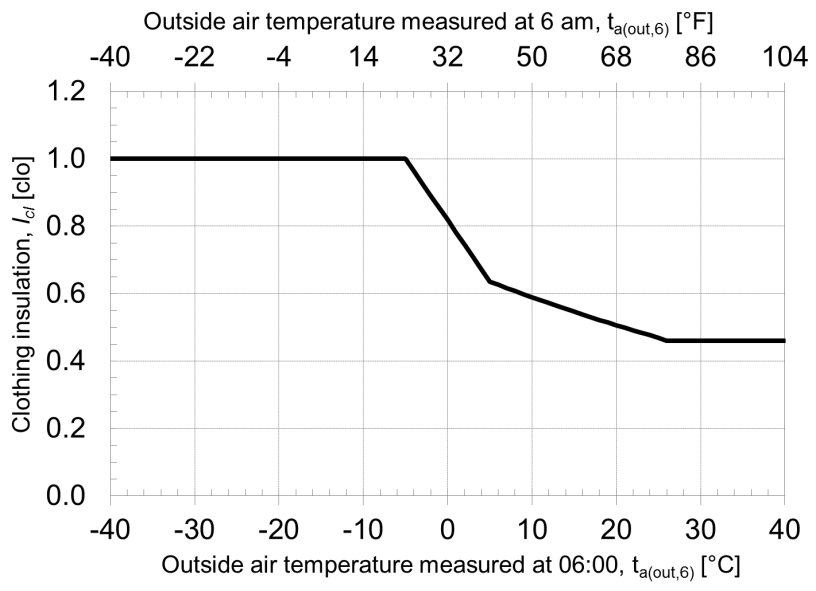
\includegraphics[width=0.9\textwidth, height=0.9\textheight, keepaspectratio=true]{media/image083.png}
\caption{Graphical representation fo the dynamic predictive clothing insulation model \protect \label{fig:graphical-representation-fo-the-dynamic}}
\end{figure}

\paragraph{Field: Clothing Insulation Calculation Method Schedule Name}\label{field-clothing-insulation-calculation-method-schedule-name}

This field specifies which clothing insulation method (ClothingInsulationSchedule or DynamicClothingModelASHRAE55) to use at a particular time of the day. A schedule value of 1 means the ClothingInsulationSchedule method, and 2 means the DynamicClothingModelASHRAE55 method. This field is only required when the ``Clothing Insulation Calculation Method'' field is set to \textbf{CalculationMethodSchedule}. If this field is left blank, the specified clothing insulation calculation method will be used and not changed during the simulation.

\paragraph{Field: Clothing Insulation Schedule Name}\label{field-clothing-insulation-schedule-name}

This field is the name of the schedule that defines the amount of clothing being worn by a typical zone occupant during various times in the simulation period. The choice from the Clothing Insulation Calculation Method field should be ``\textbf{ClothingInsulationSchedule}''. This parameter must be a positive real number and has units of Clo. Typical values for Clo can be seen in the ASHRAE 2009 HOF Table 7, page 9.8 (for clothing ensembles) and Table~\ref{table:window-modeling-options}, page 9.9 (for garment values) ) or www.cbe.berkeley.edu/comforttool/. This field is required to run one of the following thermal comfort models: Fanger, Pierce, KSU, CoolingEffectASH55 or AnkleDraftASH55. If a schedule is listed here but no thermal comfort model is selected, then a warning message will be produced and this schedule will be listed as unused in the error file.

\paragraph{Field: Air Velocity Schedule Name}\label{field-air-velocity-schedule-name}

This field is the name of the schedule that approximates the amount of air movement in the space as a function of time throughout the simulation period. The user has control over this parameter through the schedule that requires the individual numbers in the schedule to be positive real numbers having units of meters per second. This field is required to run one of the following thermal comfort models: Fanger, Pierce, KSU, CoolingEffectASH55 or AnkleDraftASH55. If a schedule is listed here but no thermal comfort model is selected, then a warning message will be produced and this schedule will be listed as unused in the error file.

\paragraph{Field: Thermal Comfort Model Type (up to 7 allowed)}\label{field-thermal-comfort-model-type-up-to-7-allowed}

The final one to five fields are optional and are intended to trigger various thermal comfort models within EnergyPlus. By entering the keywords Fanger, Pierce, KSU, AdaptiveASH55, AdaptiveCEN15251, CoolingEffectASH55, and AnkleDraftASH55, the user can request the Fanger, Pierce Two-Node, Kansas State UniversityTwo-Node, the adaptive comfort models of the ASHRAE Standard 55 and CEN Standard 15251, ASHRAE Standard 55 Elevated Air Cooling Effect model, and ASHRAE Standard 55 Ankle Draft Risk model results for this particular people statement. Detailed descriptions and requirements of the seven models as listed below.

\begin{description}
  \item[Fanger] 
  Fanger’s Comfort model is applied to calculate related thermal comfort metrics. Fanger Model PMV, PPD, and Clothing Surface Temperature are calculated and reported as each time step. Apart from existing required fields in People object, extra fields required for this model include Surface Name/Angle Factor List Name, Work Efficiency Schedule Name, Clothing Insulation Schedule Name, and Air Velocity Schedule Name.

  \item[Pierce] 
  The Pierce Two-Node model is applied to calculate related thermal comfort metrics. Pierce Model Effective Temperature PMV, Standard Effective Temperature PMV, Discomfort Index, Thermal Sensation Index, and Standard Effective Temperature are calculated and reported as each time step.Apart from existing required fields in People object, extra fields required for this model include Surface Name/Angle Factor List Name, Work Efficiency Schedule Name, Clothing Insulation Schedule Name, and Air Velocity Schedule Name.

  \item[KSU] 
  The KSU Two-Node Model is applied to calculate related thermal comfort metrics. KSU Model Thermal Sensation Vote is calculated and reported as each time step. Note that the KSU model is computationally intensive and may noticeably increase the execution time of the simulation. Apart from existing required fields in People object, extra fields required for this model include Surface Name/Angle Factor List Name, Work Efficiency Schedule Name, Clothing Insulation Schedule Name, and Air Velocity Schedule Name.

  \item[AdaptiveASH55] 
  Adaptive Comfort Model Based on ASHRAE Standard 55-2010 is applied to calculate related thermal comfort metrics. ASHRAE 55 Adaptive Model 90\% Acceptability Status, 80\% Acceptability Status, Running Average Outdoor Air Temperature, and the Adaptive Model Temperature are calculated and reported as each time step. AdaptiveASH55 is only applicable when the running average outdoor air temperature for the past 7 days is between 10.0 and 33.5C.

  \item[AdaptiveCEN15251] 
  Adaptive Comfort Model Based on European Standard EN15251-2007 is applied to calculate related thermal comfort metrics. CEN 15251 Adaptive Model Category I/II/II Status, Running Average Outdoor Air Temperature, and the Adaptive Model Temperature are calculated and reported as each time step. AdaptiveCEN15251 is only applicable when the running average outdoor air temperature for the past 30 days is between 10.0 and 30.0C.

  \item[CoolingEffectASH55] 
  ASHRAE 55-2017 Elevated Air Speed Cooling Effect Model is applied to calculate related thermal comfort metrics. Elevated Air Speed Cooling Effect, Cooling Effect Adjusted PMV, and Cooling Effect Adjusted PPD are calculated and reported as each time step. Apart from existing required fields in People object, extra fields required for this model include Surface Name/Angle Factor List Name, Work Efficiency Schedule Name, Clothing Insulation Schedule Name, and Air Velocity Schedule Name.

  \item[AnkleDraftASH55] 
  ASHRAE 55-2017 Ankle Draft Risk Model is applied to calculate related thermal comfort metrics. Zone Thermal Comfort ASHRAE 55 Ankle Draft PPD is calculated and reported as each time step. Apart from existing required fields in People object, extra fields required for this model include Surface Name/Angle Factor List Name, Work Efficiency Schedule Name, Clothing Insulation Schedule Name, Air Velocity Schedule Name, and Ankle Level Air Velocity Schedule Name. Ankle draft PPD calculations are only applicable for relative air velocity is below 0.2 m/s, and the subject’s metabolic rate and clothing level should be kept below 1.3 met and 0.7 clo. PPD at ankle draft will be set to -1.0 if if these conditions are not met.

\end{description}

 For descriptions of the thermal comfort calculations, see the Engineering Reference document.

 Note that since up to seven models may be specified, the user may opt to have EnergyPlus calculate the thermal comfort for people identified with this people statement using all seven models if desired. 


\paragraph{Field: Ankle Level Air Velocity Schedule Name}\label{field-ankle-level-air-velocity-schedule-name}

This field is the name of the schedule that approximates the amount of air movement at the occupants' ankle level (0.1 m above floor level) as a function of time throughout the simulation period. The user has control over this parameter through the schedule that requires the individual numbers in the schedule to be positive real numbers having units of meters per second. This field is required to run the AnkleDraftASH55 thermal comfort model. If a schedule is listed here but no thermal comfort model is selected, then a warning message will be produced and this schedule will be listed as unused in the error file.

The following IDF example allows for a maximum of 31 people with scheduled occupancy of ``Office Occupancy'', 60\% radiant using an Activity Schedule of ``Activity Sch''. The example allows for thermal comfort reporting.

\begin{lstlisting}

People,
  Kitchen_ZN_1_FLR_1,   !- Name
  Kitchen_ZN_1_FLR_1,   !- Zone or ZoneList Name
  BLDG_OCC_SCH,         !- Number of People Schedule Name
  People,               !- Number of People Calculation Method
  25.2000,,,            !- Number of People, People per Zone Floor Area, Zone Floor Area per Person
  0.3000,               !- Fraction Radiant
  AUTOCALCULATE,        !- Sensible Heat Fraction
  ACTIVITY_SCH,         !- Activity Level Schedule Name
  3.82E-8,              !- Carbon Dioxide Generation Rate {m3/s-W}
  No,                   !- Enable ASHRAE 55 Comfort Warnings
  ZoneAveraged,         !- Mean Radiant Temperature Calculation Type
  ,                     !- Surface Name/Angle Factor List Name
  WORK_EFF_SCH,         !- Work Efficiency Schedule Name
  ClothingInsulationSchedule, !- Clothing Insulation Calculation Method
  ,                     !- Clothing Insulation Calculation Method Schedule Name
  CLOTHING_SCH,         !- Clothing Insulation Schedule Name
  AIR_VELO_SCH,         !- Air Velocity Schedule Name
  Fanger;               !- Thermal Comfort Model 1 Type
\end{lstlisting}

A simpler example, without using the thermal comfort reporting option:

\begin{lstlisting}
People,
  RIGHT FORK,     !- Name
  RIGHT FORK,     !- Zone or ZoneListName
  Dorm Occupancy, !- Number of People Schedule Name
  people,         !- Number of People Calculation Method
  8.00000,        !- Number of People,
  ,               !- People per Zone Floor Area
  ,               !- Zone Floor Area per Person
  0.6000000,      !- Fraction Radiant
  Autocalculate,  !- Sensible Heat Fraction
  Activity Sch,   !- Activity level Schedule Name
\end{lstlisting}

And with the sensible fraction specified:

\begin{lstlisting}
People,
  SPACE1-1 People 1,    !- Name
  SPACE1-1,             !- Zone or ZoneListName
  OCCUPY-1,             !- Number of People Schedule Name
  people,               !- Number of People Calculation Method
  11,                   !- Number of People
  ,                     !- People per Zone Floor Area
  ,                     !- Zone Floor Area per Person
  0.3,                  !- Fraction Radiant
  0.55,                 !- Sensible Heat Fraction
  ActSchd;              !- Activity level Schedule Name
\end{lstlisting}

Global People Object:

\begin{lstlisting}
ZoneList,AllOccupiedZones,SPACE1-1,SPACE2-1,SPACE3-1,SPACE4-1,SPACE5-1;

People,
  AllZones with People, !- Name
  AllOccupiedZones,     !- Zone or ZoneList Name
  OCCUPY-1,             !- Number of People Schedule Name
  People/Area,          !- Number of People Calculation Method
  ,                     !- Number of People
  .11,                  !- People per Zone Floor Area {person/m2}
  ,                     !- Zone Floor Area per Person {m2/person}
  0.3,                  !- Fraction Radiant
  ,                     !- Sensible Heat Fraction
  ActSchd,              !- Activity Level Schedule Name
  3.82E-8,              !- Carbon Dioxide Generation Rate {m3/s-W}
  No,                   !- Enable ASHRAE 55 Comfort Warnings
  surfaceweighted,      !- Mean Radiant Temperature Calculation Type
  Zn001:Wall001,        !- Surface Name/Angle Factor List Name
  Work Eff Sch,         !- Work Efficiency Schedule Name
  ClothingInsulationSchedule,  !- Clothing Insulation Calculation Method
  ,                     !- Clothing Insulation Calculation Method Schedule Name
  Clothing Sch,         !- Clothing Insulation Schedule Name
  Air Velo Sch,         !- Air Velocity Schedule Name
  FANGER,               !- Thermal Comfort Model 1 Type
  PIERCE,               !- Thermal Comfort Model 2 Type
  KSU;                  !- Thermal Comfort Model 3 Type
\end{lstlisting}

\subsubsection{Outputs}\label{outputs-017}

People objects have output variables for individual objects and for zone totals.

People specific outputs include:

\begin{itemize}
\item
  Zone,Average,People Occupant Count {[]}
\item
  Zone,Sum,People Radiant Heating Energy {[}J{]}
\item
  Zone,Average,People Radiant Heating Rate {[}W{]}
\item
  Zone,Sum,People Convective Heating Energy {[}J{]}
\item
  Zone,Average,People Convective Heating Rate {[}W{]}
\item
  Zone,Sum,People Sensible Heating Energy {[}J{]}
\item
  Zone,Average,People Sensible Heating Rate {[}W{]}
\item
  Zone,Sum,People Latent Gain Energy {[}J{]}
\item
  Zone,Average,People Latent Gain Rate {[}W{]}
\item
  Zone,Sum,People Total Heating Energy {[}J{]}
\item
  Zone,Average,People Total Heating Rate {[}W{]}
\item
  Zone,Average,Zone People Occupant Count {[]}
\item
  Zone,Sum,Zone People Radiant Heating Energy {[}J{]}
\item
  Zone,Average,Zone People Radiant Heating Rate {[}W{]}
\item
  Zone,Sum,Zone People Convective Heating Energy {[}J{]}
\item
  Zone,Average,Zone People Convective Heating Rate {[}W{]}
\item
  Zone,Sum,Zone People Sensible Heating Energy {[}J{]}
\item
  Zone,Average,Zone People Sensible Heating Rate {[}W{]}
\item
  Zone,Sum,Zone People Latent Gain Energy {[}J{]}
\item
  Zone,Average,Zone People Latent Gain Rate {[}W{]}
\item
  Zone,Sum,Zone People Total Heating Energy {[}J{]}
\item
  Zone,Average,People Air Temperature {[}C{]}
\item
  Zone,Average,People Air Relative Humidity {[}\%{]}
\item
  Zone,Average,Zone People Total Heating Rate {[}W{]}
\item
  Zone,Average,Zone Thermal Comfort Mean Radiant Temperature {[}C{]}
\item
  Zone,Average,Zone Thermal Comfort Operative Temperature {[}C{]}
\item
  Zone,Average,Zone Thermal Comfort Fanger Model PMV {[]}
\item
  Zone,Average,Zone Thermal Comfort Fanger Model PPD {[}\%{]}
\item
  Zone,Average,Zone Thermal Comfort Clothing Surface Temperature {[}C{]}
\item
  Zone,Average,Zone Thermal Comfort Pierce Model Effective Temperature PMV {[]}
\item
  Zone,Average,Zone Thermal Comfort Pierce Model Standard Effective Temperature PMV {[]}
\item
  Zone,Average,Zone Thermal Comfort Pierce Model Discomfort Index {[]}
\item
  Zone,Average,Zone Thermal Comfort Pierce Model Thermal Sensation Index {[]}
\item
  Zone,Average,Zone Thermal Comfort Pierce Model Standard Effective Temperature {[C]}
\item
  Zone,Average,Zone Thermal Comfort KSU Model Thermal Sensation Index {[]}
\item
  Zone,Average,Zone Thermal Comfort ASHRAE 55 Adaptive Model 80\% Acceptability Status {[]}
\item
  Zone,Average,Zone Thermal Comfort ASHRAE 55 Adaptive Model 90\% Acceptability Status {[]}
\item
  Zone,Average,Zone Thermal Comfort ASHRAE 55 Adaptive Model Running Average Outdoor Air Temperature {[}C{]}
\item
  Zone,Average,Zone Thermal Comfort ASHRAE 55 Adaptive Model Temperature {[}C{]}
\item
  Zone,Average,Zone Thermal Comfort CEN 15251 Adaptive Model Category I Status {[]}
\item
  Zone,Average,Zone Thermal Comfort CEN 15251 Adaptive Model Category II Status {[]}
\item
  Zone,Average,Zone Thermal Comfort CEN 15251 Adaptive Model Category III Status
\item
  Zone,Average,Zone Thermal Comfort CEN 15251 Adaptive Model Running Average Outdoor Air Temperature {[}C{]}
\item
  Zone,Average,Zone Thermal Comfort CEN 15251 Adaptive Model Temperature {[}C{]}
\item
  Zone,Average,Zone Thermal Comfort ASHRAE 55 Elevated Air Speed Cooling Effect {[}C{]}
\item
  Zone,Average,Zone Thermal Comfort ASHRAE 55 Elevated Air Speed Cooling Effect Adjusted PMV {[]}
\item
  Zone,Average,Zone Thermal Comfort ASHRAE 55 Elevated Air Speed Cooling Effect Adjusted PPD {[]}
\item
  Zone,Average,Zone Thermal Comfort ASHRAE 55 Ankle Draft PPD {[]}
\end{itemize}

It should be noted that if a user is trying to output the Standard Effective Temperature (SET) that the Pierce two-node model must be selected.  This variable is calculated as part of the Pierce model and can be seen in the output by requesting Zone Thermal Comfort Pierce Model Standard Effective Temperature.

\paragraph{People Occupant Count {[]}}\label{people-occupant-count}

This field is the number of people for this PEOPLE object during the timestep in question.

\paragraph{People Radiant Heating Rate {[}W{]}}\label{people-radiant-heating-rate-w}

\paragraph{People Radiant Heating Energy {[}J{]}}\label{people-radiant-heating-energy-j}

These output variables are the amount of radiant heat gain for this People object in Watts (for rate) or Joules. This is determined by the current sensible heat gain from people to the zone and the ``Fraction Radiant'' specified in the input. The radiant gains from people are distributed to the surfaces using an area weighting scheme.

\paragraph{People Convective Heating Rate {[}W{]}}\label{people-convective-heating-rate-w}

\paragraph{People Convective Heating Energy {[}J{]}}\label{people-convective-heating-energy-j}

These output variables are the amount of convective heat gain for this People object in Watts (for rate) or Joules. This is determined by the current sensible heat gain from people to the zone and the ``Fraction Radiant'' specified in input. Note that the radiant and convective gains should add up to the sensible heat gain from people. The convective heat gain from people is added to the zone air heat balance directly.

\paragraph{People Latent Gain Rate {[}W{]}}\label{people-latent-gain-rate-w}

\paragraph{People Latent Gain Energy {[}J{]}}\label{people-latent-gain-energy-j}

These output variables are the amount of latent heat gain for this People object in Watts (for rate) or Joules. This amount is based on the number of people in the space as well as the total amount of energy produced by a typical person defined by the activity schedule in the input. An internal algorithm is used to determine what fraction of the total is sensible and what fraction is latent. Details about this split are included in the Engineering Reference document.

\paragraph{People Sensible Heating Rate {[}W{]}}\label{people-sensible-heating-rate-w}

\paragraph{People Sensible Heating Energy {[}J{]}}\label{people-sensible-heating-energy-j}

These output variables are the amount of sensible heat gain for this People object in Watts (for rate) or Joules. This amount is based on the number of people in the space as well as the total amount of energy produced by a typical person defined by the activity schedule in the input. An internal algorithm (described in the Engineering Reference document) is used to determine what fraction of the total is sensible and what fraction is latent. The sensible plus the latent heat gain from people equals the total gain specified in the input.

\paragraph{People Total Heating Rate {[}W{]}}\label{people-total-heating-rate-w}

\paragraph{People Total Heating Energy {[}J{]}}\label{people-total-heating-energy-j}

These output variables are the total amount of heat gain for this People object in Watts (for rate) or Joules. This is derived from the activity level times the number of occupants.

\paragraph{People Air Temperature {[}C{]}}\label{people-air-temperature-c}

This output variable represents the zone air temperature based on the Fanger thermal comfort model.~ If there is a ZoneControl:Thermostat:ThermalComfort object specified and the thermal zone is occupied, then the value of ``People Air Temperature'' is determined based on the thermal comfort that satisfies the thermal comfort setpoint PMV value specified; otherwise, it is set to average zone air temperature.

\paragraph{People Air Relative Humidity {[}\%{]}}\label{people-air-relative-humidity}

This output variable represents the zone air relative humidity based on the Fanger thermal comfort model.~ If there is a ZoneControl:Thermostat:ThermalComfort object specified and the thermal zone is occupied, then the value of ``People Air Relative Humidity'' is determined from the mean zone air temperature and zone air humidity ratio that satisfies the thermal comfort setpoint PMV value specified; otherwise, it is calculated from the zone air temperature and humidity ratio averaged over the time step.

\paragraph{Zone People Occupant Count {[]}}\label{zone-people-occupant-count}

This field is the total number of people within the zone during the timestep in question.

\paragraph{Zone People Radiant Heating Rate {[}W{]}}\label{zone-people-radiant-heating-rate-w}

\paragraph{Zone People Radiant Heating Energy {[}J{]}}\label{zone-people-radiant-heating-energy-j}

These output variables are the amount of radiant heat gain from people within the zone in Watts (for rate) or Joules. This is determined by the current sensible heat gain from people to the zone and the ``Fraction Radiant'' specified in the input. The radiant gains from people are distributed to the surfaces using an area weighting scheme.

\paragraph{Zone People Convective Heating Rate {[}W{]}}\label{zone-people-convective-heating-rate-w}

\paragraph{Zone People Convective Heating Energy {[}J{]}}\label{zone-people-convective-heating-energy-j}

These output variables are the amount of convective heat gain from people within the zone in Watts (for rate) or Joules. This is determined by the current sensible heat gain from people to the zone and the ``Fraction Radiant'' specified in input. Note that the radiant and convective gains should add up to the sensible heat gain from people. The convective heat gain from people is added to the zone air heat balance directly.

\paragraph{Zone People Latent Gain Rate {[}W{]}}\label{zone-people-latent-gain-rate-w}

\paragraph{Zone People Latent Gain Energy {[}J{]}}\label{zone-people-latent-gain-energy-j}

These output variables are the amount of latent heat gain from people within the zone in Watts (for rate) or Joules. This amount is based on the number of people in the space as well as the total amount of energy produced by a typical person defined by the activity schedule in the input. An internal algorithm is used to determine what fraction of the total is sensible and what fraction is latent. Details about this split are included in the Engineering Reference document.

\paragraph{Zone People Sensible Heating Rate {[}W{]}}\label{zone-people-sensible-heating-rate-w}

\paragraph{Zone People Sensible Heating Energy {[}J{]}}\label{zone-people-sensible-heating-energy-j}

These output variables are the amount of sensible heat gain from people within the zone in Watts (for rate) or Joules. This amount is based on the number of people in the space as well as the total amount of energy produced by a typical person defined by the activity schedule in the input. An internal algorithm (described in the Engineering Reference document) is used to determine what fraction of the total is sensible and what fraction is latent. The sensible plus the latent heat gain from people equals the total gain specified in the input.

\paragraph{Zone People Total Heating Rate {[}W{]}}\label{zone-people-total-heating-rate-w}

\paragraph{Zone People Total Heating Energy {[}J{]}}\label{zone-people-total-heating-energy-j}

These output variables are the total amount of heat gain from people within the zone in Watts (for rate) or Joules. Derived from the activity level times the number of occupants, this is summed for each people object within a zone.

\paragraph{Zone Thermal Comfort Mean Radiant Temperature {[}C{]}}\label{zone-thermal-comfort-mean-radiant-temperature-c}

This output variable is the mean radiant temperature used in the thermal comfort calculations.~ This value is computed according to the ``MRT Calculation Type'' specified in the PEOPLE object.~ If a high temperature radiant system is present in the zone, this value will be adjusted according to the current heater operation and the ``Fraction of radiant energy incident on people'' specified in the HIGH TEMP RADIANT SYSTEM object.

\paragraph{Zone Thermal Comfort Operative Temperature {[}C{]}}\label{zone-thermal-comfort-operative-temperature-c}

This output variable is the operative temperature as defined by the thermal comfort operations. Specifically, it is the average of the thermal comfort mean radiant temperature and the zone air temperature.

Note for all Thermal Comfort reporting:~ Though the published values for thermal comfort ``vote'' have a discrete scale (e.g. --3 to +3 or --4 to +4), the calculations in EnergyPlus are carried out on a continuous scale and, thus, reporting may be ``off the scale'' with specific conditions encountered in the space. This is not necessarily an error in EnergyPlus -- rather a different approach that does not take the ``limits'' of the discrete scale values into account.

\paragraph{Zone Thermal Comfort Fanger Model PMV {[]}}\label{zone-thermal-comfort-fanger-model-pmv}

This field is the ``predicted mean vote'' (PMV) calculated using the Fanger thermal comfort model. Details on the equations used to calculate the Fanger PMV are shown in the EnergyPlus Engineering Reference. If the zone in question is currently being controlled using a thermostat object, then the value of the PMV is determined by using the air temperature and humidity that is calculated at the system time step; otherwise, if the zone is uncontrolled, the PMV is determined using the zone air temperature and humidity that is averaged over the zone time step.

\paragraph{Zone Thermal Comfort Fanger Model PPD {[}\%{]}}\label{zone-thermal-comfort-fanger-model-ppd}

This field is the ``predicted percentage of dissatisfied'' (PPD) calculated using the Fanger thermal comfort model.  Details on the equations used to calculate the Fanger PPD are shown in the EnergyPlus Engineering Reference. If the zone in question is currently being controlled using a thermostat object, then the value of the PPD is determined by using the air temperature and humidity that is calculated at the system time step; otherwise, if the zone is uncontrolled, the PPD is determined using the zone air temperature and humidity that is averaged over the zone time step.

\paragraph{Zone Thermal Comfort Clothing Surface Temperature {[}C{]}}\label{zone-thermal-comfort-clothing-surface-temperature-c}

This output variable is the calculation of the clothing surface temperature using the Fanger thermal comfort model.

\paragraph{Zone Thermal Comfort Pierce Model Effective Temperature PMV {[]}}\label{zone-thermal-comfort-pierce-model-effective-temperature-pmv}

This field is the ``predicted mean vote'' (PMV) calculated using the effective temperature and the Pierce two-node thermal comfort model.

\paragraph{Zone Thermal Comfort Pierce Model Standard Effective Temperature PMV {[]}}\label{zone-thermal-comfort-pierce-model-standard-effective-temperature-pmv}

This field is the ``predicted mean vote'' (PMV) calculated using the ``standard'' effective temperature and the Pierce two-node thermal comfort model.

\paragraph{Zone Thermal Comfort Pierce Model Discomfort Index {[]}}\label{zone-thermal-comfort-pierce-model-discomfort-index}

This field is the ``discomfort index'' calculated using the the Pierce two-node thermal comfort model.

\paragraph{Zone Thermal Comfort Pierce Model Thermal Sensation Index {[]}}\label{zone-thermal-comfort-pierce-model-thermal-sensation-index}

This field is the ``thermal sensation index'' (PMV) calculated using the Pierce two-node thermal comfort model.

\paragraph{Zone Thermal Comfort Pierce Model Standard Effective Temperature {[C]}}\label{zone-thermal-comfort-pierce-model-standard-effective-temperature}

This field is the ``standard effective temperature'' (SET) calculated using the Pierce two-node thermal comfort model.  Note that if a user wishes to report the Pierce Model SET that it must be done using the Pierce two-node model and the user must select ``Pierce'' as one of the Thermal Comfort model types as shown above in the input syntax for the People statement.

\paragraph{Zone Thermal Comfort KSU Model Thermal Sensation Vote {[]}}\label{zone-thermal-comfort-ksu-model-thermal-sensation-vote}

This field is the ``thermal sensation vote'' (TSV) calculated using the KSU two-node thermal comfort model.

\paragraph{Zone Thermal Comfort ASHRAE 55 Adaptive Model 90\% Acceptability Status {[]}}\label{zone-thermal-comfort-ashrae-55-adaptive-model-90-acceptability-status}

This field is to report whether the operative temperature falls into the 90\% acceptability limits of the adaptive comfort in ASHRAE 55-2010. A value of 1 means within (inclusive) the limits, a value of 0 means outside the limits, and a value of -1 means not applicable (when unoccupied or running average outdoor temp is outside the range of 10.0 to 33.5C).

\paragraph{Zone Thermal Comfort ASHRAE 55 Adaptive Model 80\% Acceptability Status {[]}}\label{zone-thermal-comfort-ashrae-55-adaptive-model-80-acceptability-status}

This field is to report whether the operative temperature falls into the 80\% acceptability limits of the adaptive comfort in ASHRAE 55-2010. A value of 1 means within (inclusive) the limits, a value of 0 means outside the limits, and a value of -1 means not applicable (when unoccupied or running average outdoor temp is outside the range of 10.0 to 33.5C).

\paragraph{Zone Thermal Comfort ASHRAE 55 Adaptive Model Running Average Outdoor Air Temperature {[}C{]}}\label{zone-thermal-comfort-ashrae-55-adaptive-model-running-average-outdoor-air-temperature-c}

This field reports the mean monthly outdoor air temperature, an input parameter for the ASHRAE-55 adaptive comfort model. This can be computed in two ways. If the .stat file is provided for the simulation, this field will reflect the monthly daily average temperature.

If the .epw file is used, the field reports the simple running average of the daily average outdoor dry-bulb temperatures of the previous 30 days.

\paragraph{Zone Thermal Comfort ASHRAE 55 Adaptive Model Temperature {[}C{]}}\label{zone-thermal-comfort-ashrae-55-adaptive-model-temperature-c}

This field reports the ideal indoor operative temperature, or comfort temperature, as determined by the ASHRAE-55 adaptive comfort model. The 80\% acceptability limits for indoor operative temperature are defined as no greater than 3.5 degrees C from the adaptive comfort temperature. The 90\% acceptability limits are defined as no greater than 2.5 degrees C from the adaptive comfort temperature. A value of -1 means not applicable (when running average outdoor temp is outside the range of 10.0 to 33.5C).

\paragraph{Zone Thermal Comfort CEN 15251 Adaptive Model Category I Status}\label{zone-thermal-comfort-cen-15251-adaptive-model-category-i-status}

This field is to report whether the operative temperature falls into the Category I (90\% acceptability) limits of the adaptive comfort in the European Standard EN15251-2007. A value of 1 means within (inclusive) the limits, a value of 0 means outside the limits, and a value of -1 means not applicable (when unoccupied or running average outdoor temp is outside the range of 10.0 to 30.0C).

\paragraph{Zone Thermal Comfort CEN 15251 Adaptive Model Category II Status}\label{zone-thermal-comfort-cen-15251-adaptive-model-category-ii-status}

This field is to report whether the operative temperature falls into the Category II (80\% acceptability) limits of the adaptive comfort in the European Standard EN15251-2007. A value of 1 means within (inclusive) the limits, a value of 0 means outside the limits, and a value of -1 means not applicable (when unoccupied or running average outdoor temp is outside the range of 10.0 to 30.0C).

\paragraph{Zone Thermal Comfort CEN 15251 Adaptive Model Category III Status}\label{zone-thermal-comfort-cen-15251-adaptive-model-category-iii-status}

This field is to report whether the operative temperature falls into the Category III (65\% acceptability) limits of the adaptive comfort in the European Standard EN15251-2007. A value of 1 means within (inclusive) the limits, a value of 0 means outside the limits, and a value of -1 means not applicable (when unoccupied or running average outdoor temp is outside the range of 10.0 to 30.0C).

\paragraph{Zone Thermal Comfort CEN 15251 Adaptive Model Running Average Outdoor Air Temperature}\label{zone-thermal-comfort-cen-15251-adaptive-model-running-average-outdoor-air-temperature}

This field reports the weighted average of the outdoor air temperature of the previous seven days, an input parameter for the CEN-15251 adaptive comfort model.

\paragraph{Zone Thermal Comfort CEN 15251 Adaptive Model Temperature}\label{zone-thermal-comfort-cen-15251-adaptive-model-temperature}

This field reports the ideal indoor operative temperature, or comfort temperature, as determined by the CEN-15251 adaptive comfort model. Category I, II, and II limits for indoor operative temperature are defined as no greater than 2, 3, and 4 degrees C from this value respectively. A value of -1 means not applicable (when running average outdoor temp is outside the range of 10.0 to 30.0C).

\paragraph{Zone Thermal Comfort ASHRAE 55 Elevated Air Speed Cooling Effect}\label{zone-thermal-comfort-ashrae55-elevated-air-speed-cooling-effect}

This field is the calculated Cooling Effect of the elevated air speed in degree celsius. It is the value that, when subtracted equally from both the average air temperature and the mean radiant temperature, yields the same SET under still air as in the first SET calculation under elevated air speed.

\paragraph{Zone Thermal Comfort ASHRAE 55 Elevated Air Speed Cooling Effect Adjusted PMV}\label{zone-thermal-comfort-ashrae55-elevated-air-speed-cooling-effect-adjusted-pmv}

This field is the ``predicted mean vote'' (PMV) calculated using the Fanger PMV model, adjusted by the ASHRAE 55 Elevated Air Speed Cooling Effect. The Cooling Effect adjusted PMV for an environment with elevated average air speed is calculated using the adjusted average air temperature, the adjusted radiant temperature, and still air (0.1 m/s). 

\paragraph{Zone Thermal Comfort ASHRAE 55 Elevated Air Speed Cooling Effect Adjusted PPD}\label{zone-thermal-comfort-ashrae55-elevated-air-speed-cooling-effect-adjusted-ppd}

This field is the ``predicted percentage of dissatisfied'' (PPD) calculated using the Fanger PMV-PPD model, adjusted by the ASHRAE 55 Elevated Air Speed Cooling Effect. The Cooling Effect adjusted PPD for an environment with elevated average air speed is calculated using the adjusted average air temperature, the adjusted radiant temperature, and still air (0.1 m/s). 

\paragraph{Zone Thermal Comfort ASHRAE 55 Ankle Draft PPD}\label{zone-thermal-comfort-ashrae55-ankle-draft-ppd}

This field is the ``ppredicted percentage of dissatisfied'' (PPD) on draft at ankle level. It is used as the metric to evaluate the ankle draft risk as a function of PMV and air speed at the ankle level (0.1 m). 

\subsubsection{Outputs}\label{outputs-1-014}

The following output variables are all based on whether the humidity ratio and the operative temperature is within the region shown in ASHRAE Standard 55-2004 in Figure 5.2.1.1. For these outputs the operative temperature is simplified to be the average of the air temperature and the mean radiant temperature. For summer, the 0.5 Clo level is used and, for winter, the 1.0 Clo level is used. The graphs below are based on the following tables which extend the ASHRAE values to zero humidity ratio.

% table 12
\begin{longtable}[c]{@{}ll@{}}
\caption{Winter Clothes (1.0 Clo) \label{table:winter-clothes-1.0-clo}} \tabularnewline
\toprule
Operative Temperature (C) & Humidity Ratio (kgWater/kgDryAir) \tabularnewline
\midrule
\endfirsthead

\caption[]{Winter Clothes (1.0 Clo)} \tabularnewline
\toprule
Operative Temperature (C) & Humidity Ratio (kgWater/kgDryAir) \tabularnewline
\midrule
\endhead

19.6 & 0.012 \tabularnewline
23.9 & 0.012 \tabularnewline
26.3 & 0.000 \tabularnewline
21.7 & 0.000 \tabularnewline
\bottomrule
\end{longtable}

\begin{figure}[hbtp] % fig 49
\centering
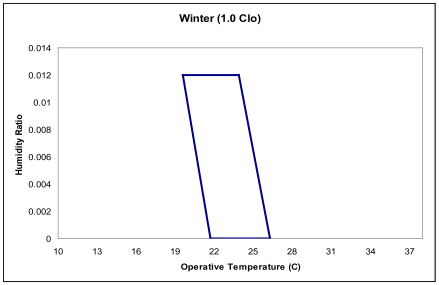
\includegraphics[width=0.9\textwidth, height=0.9\textheight, keepaspectratio=true]{media/image084.png}
\caption{Winter Comfort Range \protect \label{fig:winter-comfort-range}}
\end{figure}

% table 13
\begin{longtable}[c]{@{}ll@{}}
\caption{Summer Clothes (0.5 Clo) \label{table:summer-clothes-0.5-clo}} \tabularnewline
\toprule
Operative Temperature (C) & Humidity Ratio (kgWater/kgDryAir) \tabularnewline
\midrule
\endfirsthead

\caption[]{Summer Clothes (0.5 Clo)} \tabularnewline
\toprule
Operative Temperature (C) & Humidity Ratio (kgWater/kgDryAir) \tabularnewline
\midrule
\endhead

23.6 & 0.012 \tabularnewline
26.8 & 0.012 \tabularnewline
28.3 & 0.000 \tabularnewline
25.1 & 0.000 \tabularnewline
\bottomrule
\end{longtable}

\begin{figure}[hbtp] % fig 50
\centering
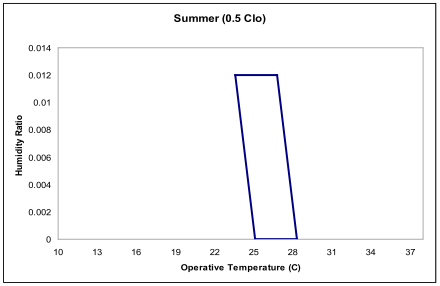
\includegraphics[width=0.9\textwidth, height=0.9\textheight, keepaspectratio=true]{media/image085.png}
\caption{Summer Comfort Range \protect \label{fig:summer-comfort-range}}
\end{figure}

\paragraph{Zone Thermal Comfort ASHRAE 55 Simple Model Summer Clothes Not Comfortable Time{[}hr{]}}\label{zone-thermal-comfort-ashrae-55-simple-model-summer-clothes-not-comfortable-timehr}

The time when the zone is occupied that the combination of humidity ratio and operative temperature is not in the ASHRAE 55-2004 summer clothes region (see above)

\paragraph{Zone Thermal Comfort ASHRAE 55 Simple Model Winter Clothes Not Comfortable Time{[}hr{]}}\label{zone-thermal-comfort-ashrae-55-simple-model-winter-clothes-not-comfortable-timehr}

The time when the zone is occupied that the combination of humidity ratio and operative temperature is not in the ASHRAE 55-2004 winter clothes region (see above)

\paragraph{Zone Thermal Comfort ASHRAE 55 Simple Model Summer or Winter Clothes Not Comfortable Time{[}hr{]}}\label{zone-thermal-comfort-ashrae-55-simple-model-summer-or-winter-clothes-not-comfortable-timehr}

The time when the zone is occupied that the combination of humidity ratio and operative temperature is not in the ASHRAE 55-2004 summer or winter clothes region (see above)

\paragraph{Facility Thermal Comfort ASHRAE 55 Simple Model Summer Clothes Not Comfortable Time{[}hr{]}}\label{facility-thermal-comfort-ashrae-55-simple-model-summer-clothes-not-comfortable-timehr}

The time when any zone is occupied that the combination of humidity ratio and operative temperature is not in the ASHRAE 55-2004 summer clothes region (see above)

\paragraph{Facility Thermal Comfort ASHRAE 55 Simple Model Winter Clothes Not Comfortable Time {[}hr{]}}\label{facility-thermal-comfort-ashrae-55-simple-model-winter-clothes-not-comfortable-time-hr}

The time when any zone is occupied that the combination of humidity ratio and operative temperature is not in the ASHRAE 55-2004 winter clothes region (see above)

\paragraph{Facility Thermal Comfort ASHRAE 55 Simple Model Summer or Winter Clothes Not Comfortable Time {[}hr{]}}\label{facility-thermal-comfort-ashrae-55-simple-model-summer-or-winter-clothes-not-comfortable-time-hr}

The time when any zone is occupied that the combination of humidity ratio and operative temperature is not in the ASHRAE 55-2004 summer or winter clothes region (see above)

\subsection{Simplified ASHRAE 55 Warnings}\label{simplified-ashrae-55-warnings}

The simplified ASHRAE 55 calculations may be computed for occupied zones and, possibly, warnings are shown on the .err file at the end of each simulated environment. To enable this option set the ``Enable ASHRAE 55 comfort warnings'' field of the \hyperref[people]{People} object to Yes. These warnings will not be generated by default.

If you enable the warnings, the simplified ASHRAE 55 calculations are done for occupied zones and, possibly, warnings are shown on the .err file at the end of each simulated environment.

\begin{lstlisting}
** Warning ** More than 4% of time (350.4 hours) uncomfortable in zone ZSF1
** ~~~ ** 553.0 hours were uncomfortable based on ASHRAE 55-2004 graph (Section 5.2.1.1)
** ~~~ ** During Environment [10/01 - 09/30]: CHICAGO IL USA TMY2-94846 WMO\# = 725300
** Warning ** More than 4% of time (350.4 hours) uncomfortable in zone ZNF1
** ~~~ ** 827.8 hours were uncomfortable based on ASHRAE 55-2004 graph (Section 5.2.1.1)
** ~~~ ** During Environment [10/01 - 09/30]: CHICAGO IL USA TMY2-94846 WMO\# = 725300
** Warning ** More than 4% of time (350.4 hours) uncomfortable in zone ZSF2
** ~~~ ** 593.5 hours were uncomfortable based on ASHRAE 55-2004 graph (Section 5.2.1.1)
** ~~~ ** During Environment [10/01 - 09/30]: CHICAGO IL USA TMY2-94846 WMO\# = 725300
** Warning ** More than 4% of time (350.4 hours) uncomfortable in zone ZNF2
** ~~~ ** 875.8 hours were uncomfortable based on ASHRAE 55-2004 graph (Section 5.2.1.1)
** ~~~ ** During Environment [10/01 - 09/30]: CHICAGO IL USA TMY2-94846 WMO\# = 725300
\end{lstlisting}

You may decide if you need to change parameters to reduce these ``uncomfortable'' hours. The individual output variables shown previously may help you get more details on when these are occurring.

Following are some suggestions that might be applicable:

\begin{itemize}
\item
  Eliminate occupancy when conditioning equipment is off.
\item
  Note that the ASHRAE graph lower limit is (19.6C to 21.7C) -- heating setpoints may need to be nearer 22.2C (72F) than 21.1C (70F).
\item
  Unoccupied heating setpoint should be nearer 16.7C (62F) rather than 12.8C (55F) to reduce the start up recovery.
\item
  Start the occupied setpoint schedule, fan availability schedule, cooling pump availability schedule, reheat coil availability, one hour before occupancy. Seasonal turn on and off of equipment may cause more warnings (but potentially more energy consumption).
\item
  Unoccupied cooling setpoint should be nearer 29.4C (85F) rather than 40.0 (104F) to reduce the start up recovery.
\end{itemize}

\subsection{ComfortViewFactorAngles}\label{comfortviewfactorangles}

When requesting EnergyPlus to do a thermal comfort calculation, the program user has three options for defining how the mean radiant temperature will be calculated. The user may select ``zoneaveraged'' which results in a mean radiant temperature that is characteristic of an ``average'' location near the center of the zone. The user may also elect to place the person near a particular surface by selecting ``surfaceweighted'' in the \hyperref[people]{People} statement. This takes the average of the zone mean radiant temperature and the temperature of the surface that the person is near and uses this value as the mean radiant temperature when calculating thermal comfort.

The third option is for the user to more explicitly position the person within the space by defining the angle factors from the person to the various surfaces in the zone. This option requires the user to list the surfaces that the person can see from a radiation standpoint and also define the angle (or view) factor for each surface. The AngleFactorList input line is intended to give the user this opportunity.

\subsubsection{Inputs}\label{inputs-1-023}

\paragraph{Field: Name}\label{field-name-1-022}

This field is an unique user assigned name for the list of surfaces that can be seen radiantly by the person for whom thermal comfort is to be evaluated. Any reference to this list by a \hyperref[people]{People} statement will use this name.

\paragraph{Field: Zone Name}\label{field-zone-name-007}

Zone Name for this surface list. Each of the surfaces listed must be in this zone.

\paragraph{Field: Surface \textless{}\#\textgreater{} Name}\label{field-surface-name-002}

This field is the name of a surface in the zone seen by the person.

\paragraph{Field: Angle Factor \textless{}\#\textgreater{}}\label{field-angle-factor}

This field is the fraction that this surface contributes to the total mean radiant temperature. This can be thought of as a weighting factor for this surface and the actual mean radiant temperature used in the thermal comfort model is simply the sum of all angle factors multiplied by the corresponding inside surface temperature. The sum of all angle factors within any angle factor list must equal unity, otherwise the program will not accept the input as valid.

Note that the Surface Name/Angle Factor pair is extensible to accommodate as many
surfaces as required.

An example IDF with an electric low temperature radiant system is shown below.

\begin{lstlisting}
ComfortViewFactorAngles,
  South Zone Angle Factors, !- name of angle factor list
  South Zone,           !- Zone Name
  Zn001:Flr001,         !- Surface name 1
  0.75,                 !- Angle factor for surface 1
  Zn001:Wall001,        !- Surface name 2
  0.15,                 !- Angle factor for surface 2
  Zn001:Roof001,        !- Surface name 3
  0.10;                 !- Angle factor for surface 3
\end{lstlisting}

\subsection{Lights}\label{lights-000}

The Lights statement allows you to specify information about a zone's electric lighting system, including design power level and operation schedule, and how the heat from lights is distributed thermally.

A zone may have multiple Lights statements. For example, one statement may describe the general lighting in the zone and another the task lighting. Or you can use multiple Lights statements for a zone that has two or more general lighting systems that differ in design level, schedule, etc.

\subsubsection{Inputs}\label{inputs-2-021}

\paragraph{Field: Name}\label{field-name-2-020}

The name of the Lights object.

\paragraph{Field: Zone or ZoneList Name}\label{field-zone-or-zonelist-name-1-000}

The field is the name of the thermal zone (ref: Zone) or \hyperref[zonelist]{ZoneList} (ref: ZoneLIst) and links this Lights statement to a thermal zone or set of thermal zones in the buidling. When the \hyperref[zonelist]{ZoneList} option is used then this lights definition is applied to each of the zones in the zone list effecting a global definition for the amount of light wattage in the zone. The Zonelist option can be used effectively with the watts/area and watts/person options of the Design Level Calculation Method.

The name of the actual lights object becomes \textless{}Zone Name\textgreater{} \textless{}Lights Object Name\textgreater{} and should be less than the standard length (100 characters) for a name field. If it is greater than this standard length, it may be difficult to specify in output reporting as it will be truncated. A warning will be shown if the generated name is greater than 100 characters. If it duplicates another such concatenated name, there will be a severe error and terminate the run.

\paragraph{Field: Schedule Name}\label{field-schedule-name-002}

The name of the schedule that modifies the lighting power design level (see Design Level Calculation Method field and related subsequent fields). The schedule values can be any positive number. The electrical input for lighting in a particular timestep is the product of the design level and the value of this schedule in that timestep. If the design level is the maximum lighting power input the schedule should contain values between 0.0 and 1.0.

\paragraph{Field: Design Level Calculation Method}\label{field-design-level-calculation-method}

This field is a key/choice field that tells which of the next three fields are filled and is descriptive of the method for calculating the nominal lighting level in the Zone. The key/choices are:

\begin{itemize}
\tightlist
\item
  LightingLevel
\end{itemize}

With this choice, the method used will be a straight insertion of the lighting level (Watts) for the Zone.~ (The Lighting Level field should be filled.)

\begin{itemize}
\tightlist
\item
  Watts/Area
\end{itemize}

With this choice, the method used will be a factor per floor area of the zone. (The Watts per Zone Floor Area field should be filled).

\begin{itemize}
\tightlist
\item
  Watts/Person
\end{itemize}

With this choice, the method used will be a factor of lighting level (watts) per person. (The Watts per person field should be filled).

\paragraph{Field: Lighting Level}\label{field-lighting-level}

This is typically the maximum electrical power input (in Watts) to lighting in a zone, including ballasts, if present. This value is multiplied by a schedule fraction (see previous field) to get the lighting power in a particular timestep. In EnergyPlus, this is slightly more flexible in that the lighting design level could be a ``diversity factor'' applied to a schedule of real numbers.

\paragraph{Field: Watts per Zone Floor Area}\label{field-watts-per-zone-floor-area}

This factor (watts/m\(^{2}\)) is used, along with the Zone Floor Area to determine the maximum lighting level as described in the Lighting Level field. The choice from the method field should be ``watts/area''.

\paragraph{Field: Watts per Person}\label{field-watts-per-person}

This factor (watts/person) is used, along with the number of occupants (people) to determine the maximum lighting level as described in the Lighting Level field. The choice from the method field should be ``watts/person''.

\paragraph{Heat Gains from Lights:}\label{heat-gains-from-lights}

The electrical input to lighting ultimately appears as heat that contributes to zone loads or to return air heat gains. In EnergyPlus this heat is divided into four different fractions. Three of these are given by the input fields Return Air Fraction, Fraction Radiant and Fraction Visible. A fourth, defined as the fraction of the heat from lights convected to the zone air, is calculated by the program as:

f\(_{convected}\) = 1.0 -- (Return Air Fraction + Fraction Radiant + Fraction Visible)

You will get an error message if Return Air Fraction + Fraction Radiant + Fraction Visible exceeds 1.0.

These fractions depend on the type of lamp and luminaire, whether the luminaire is vented to the return air, etc.

\paragraph{Field: Return Air Fraction}\label{field-return-air-fraction}

The fraction of the heat from lights that goes into the zone return air (i.e., into the zone outlet node). If the return air flow is zero or the zone has no return air system, the program will put this fraction into the zone air. Return Air Fraction should be non-zero only for luminaires that are return-air ducted~ (see Table~\ref{table:approximate-values-of-return-air-fraction} and Figure 51). (However, see the field ``Return Air Fraction Is Calculated from Plenum Temperature,'' below, for an approach to modeling the case where Return Air Fraction is caused by \emph{conduction} between a luminaire that is in contact with a return-air plenum.)

\paragraph{Field: Fraction Radiant}\label{field-fraction-radiant-1}

The fraction of heat from lights that goes into the zone as long-wave (thermal) radiation. The program calculates how much of this radiation is absorbed by the inside surfaces of the zone according the area times thermal absorptance product of these surfaces.

\paragraph{Field: Fraction Visible}\label{field-fraction-visible}

The fraction of heat from lights that goes into the zone as visible (short-wave) radiation. The program calculates how much of this radiation is absorbed by the inside surfaces of the zone according the area times solar absorptance product of these surfaces.

Approximate values of Return Air Fraction, Fraction Radiant and Fraction Visible are given in Table~\ref{table:approximate-values-of-return-air-fraction} for overhead fluorescent lighting for a variety of luminaire configurations. The data is based on ASHRAE 1282-RP ``Lighting Heat Gain Distribution in Buildings'' by Daniel E. Fisher and Chanvit Chantrasrisalai.

% table 14
\begin{longtable}[c]{p{0.8in}>{\raggedright}p{1.6in}>{\raggedright}p{0.9in}>{\raggedright}p{0.9in}>{\raggedright}p{0.9in}>{\raggedright}p{0.9in}}
\caption{Approximate values of Return Air Fraction, Fraction Radiant and Fraction Visible for overhead fluorescent lighting for different luminaire configurations. \label{table:approximate-values-of-return-air-fraction}} \tabularnewline
\toprule
Fixture No. & Luminaire Feature & Return Air Fraction & Fraction Radiant & Fraction Visible & fconvected \tabularnewline
\midrule
\endfirsthead

\caption[]{Approximate values of Return Air Fraction, Fraction Radiant and Fraction Visible for overhead fluorescent lighting for different luminaire configurations.} \tabularnewline
\toprule
Fixture No. & Luminaire Feature & Return Air Fraction & Fraction Radiant & Fraction Visible & \(f_{\rm{convected}}\) \tabularnewline
\midrule
\endhead

1 & Recessed, Parabolic Louver, Non-Vented, T8 & 0.31 & 0.22 & 0.20 & 0.27 \tabularnewline
2 & Recessed, Acrylic Lens, Non-Vented, T8 & 0.56 & 0.12 & 0.20 & 0.12 \tabularnewline
3 & Recessed, Parabolic Louver, Vented, T8 & 0.28 & 0.19 & 0.20 & 0.33 \tabularnewline
4 & Recessed, Acrylic Lens, Vented, T8 & 0.54 & 0.10 & 0.18 & 0.18 \tabularnewline
5 & Recessed, Direct/Indirect, T8 & 0.34 & 0.17 & 0.16 & 0.33 \tabularnewline
6 & Recessed, Volumetric, T5 & 0.54 & 0.13 & 0.20 & 0.13 \tabularnewline
7 & Downlights, Compact Fluorescent, DTT & 0.86 & 0.04 & 0.10 & 0.00 \tabularnewline
8 & Downlights, Compact Fluorescent, TRT & 0.78 & 0.09 & 0.13 & 0.00 \tabularnewline
9a & Downlights, Incandescent, A21 & 0.29 & 0.10 & 0.6 & 0.01 \tabularnewline
9b & Downlights, Incandescent, BR40 & 0.21 & 0.08 & 0.71 & 0.00 \tabularnewline
10 & Surface Mounted, T5HO & 0.00 & 0.27 & 0.23 & 0.50 \tabularnewline
11 & Pendant, Direct/Indirect, T8 & 0.00 & 0.32 & 0.23 & 0.45 \tabularnewline
12 & Pendant, Indirect, T5HO & 0.00 & 0.32 & 0.25 & 0.43 \tabularnewline
 &  &  &  &  &  \tabularnewline \midrule
1 & Recessed, Parabolic Louver, Non-Vented, T8 - Ducted & 0.27 & 0.27 & 0.21 & 0.25 \tabularnewline
5 & Recessed, Direct/Indirect, T8 - Ducted & 0.27 & 0.22 & 0.17 & 0.34 \tabularnewline
 &  &  &  &  &  \tabularnewline \midrule
1 & Recessed, Parabolic Louver, Non-Vented, T8 - Half Typical Supply Airflow Rate & 0.45 & 0.30 & 0.22 & 0.03 \tabularnewline
3 & Recessed, Parabolic Louver, Vented, T8 - Half Typical Supply Airflow Rate & 0.43 & 0.25 & 0.21 & 0.11 \tabularnewline
5 & Recessed, Direct/Indirect, T8 - Half Typical Supply Airflow Rate & 0.43 & 0.27 & 0.18 & 0.12 \tabularnewline
 &  &  &  &  &  \tabularnewline \midrule
1 & Recessed, Parabolic Louver, Non-Vented, T8 - Half Typical Supply Airflow Rate & 0.10 & 0.16 & 0.20 & 0.54 \tabularnewline
3 & Recessed, Parabolic Louver, Vented, T8 - Half Typical Supply Airflow Rate & 0.11 & 0.15 & 0.19 & 0.55 \tabularnewline
5 & Recessed, Direct/Indirect, T8 - Half Typical Supply Airflow Rate & 0.04 & 0.13 & 0.16 & 0.67 \tabularnewline
\bottomrule
\end{longtable}

\paragraph{Field: Fraction Replaceable}\label{field-fraction-replaceable}

This field defines the daylighting control for the LIGHTS object.

If \textbf{\hyperref[daylightingcontrols-000]{Daylighting:Controls}} is specified for the zone, this field is used as an on/off flag for dimming controls. If set to 0.0, the lights are not dimmed by the daylighting controls. If set to 1.0, the lights are allowed to be dimmed by the daylighting controls.

\paragraph{Field: End-Use Subcategory}\label{field-end-use-subcategory-002}

Allows you to specify a user-defined end-use subcategory, e.g., ``Task Lights'', ``Hall Lights'', etc. A new meter for reporting is created for each unique subcategory~ (ref: \hyperref[outputmeter-and-outputmetermeterfileonly]{Output:Meter} objects). Subcategories are also reported in the ABUPS table. If this field is omitted or blank, the lights will be assigned to the ``General'' end-use subcategory. Any text may be used here to categorize the end-uses in the ABUPS End Uses by Subcategory table and the LEED EAp2-4/5. Performance Rating Method Compliance table.

\paragraph{Field: Return Air Fraction Calculated from Plenum Temperature}\label{field-return-air-fraction-calculated-from-plenum-temperature}

Accepts values Yes or No (the default). Yes is for advanced used only. In this case the program will calculate the return air fraction by assuming that it is due to conduction of some of the light heat into the zone's return air plenum and that the amount of the conduction depends on the plenum air temperature. A Yes value should only be used for luminaires that are recessed and non-vented, as shown in Figure~\ref{fig:vertical-section-through-a-zone-and-its}.

The value you enter for the Return Air Fraction field will be ignored and you can enter, for fluorescent lighting, Fraction Radiant = 0.37 and Fraction Visible = 0.18, as indicated in Table~\ref{table:approximate-values-of-return-air-fraction}.

This feature requires that the coefficients described below be determined from measurements or detailed calculations since they are very sensitive to the luminaire type, lamp type, thermal resistance between fixture and plenum, etc.

If ``Return Air Fraction Is Calculated from Plenum Temperature'' = Yes, the return air fraction is calculated \emph{each timestep} from the following empirical correlation:

\begin{equation}
  (\rm{Return Air Fraction})_{\rm{calculated}} = C_{1} - C_{2} \times T_{\rm{plenum}}
\end{equation}

where T\(_{\rm{plenum}}\) is the previous-time-step value of the return plenum air temperature (C),

and C\(_{1}\) and C\(_{2}\) are the values of the coefficients entered in the next two fields.

To compensate for the change in the return air fraction relative to its input value, the program modifies Fraction Radiant and \(f_{\rm{convected}}\) by a scale factor such that

\begin{equation}
  (\rm{Return Air Fraction})_{\rm{calculated}} + (\rm{Fraction Radiant})_{\rm{modified}} + (f_{\rm{convected}})_{\rm{modified}} + (\rm{Fraction Visible})_{\rm{input}} = 1.0
\end{equation}

It is assumed that Fraction Visible is a constant equal to its input value.

\paragraph{Field: Return Air Fraction Function of Plenum Temperature Coefficient 1}\label{field-return-air-fraction-function-of-plenum-temperature-coefficient-1}

The coefficient C\(_{1}\) in the equation for (Return Air Fraction)\(_{calculated}\).

\paragraph{Field: Return Air Fraction Function of Plenum Temperature Coefficient 2}\label{field-return-air-fraction-function-of-plenum-temperature-coefficient-2}

The coefficient C\(_{2}\) in the equation for (Return Air Fraction)\(_{calculated}\). Its units are 1/\(^{O}\)C.

\paragraph{Field: Return Air Heat Gain Node Name}\label{field-return-air-heat-gain-node-name}

Name of the return air node for this heat gain. If left blank, it defaults to the first return air node for the zone containing this Lights object. Leave blank when using a \hyperref[zonelist]{ZoneList} name.

\paragraph{Field:Exhaust Air Heat Gain Node Name}\label{field-exhaust-air-heat-gain-node-name}

Name of the exhaust air node for this heat gain. If left blank, no heat gain from retun air fraction will be added to the zone exhast node. When the exhaust node name is entered, the return air heat gain will be shared by both return and exhast nodes. The equipment can draw air from the exhaust node, but the inlet air properties is combined properties with mixing mass flow rates of both nodes and added lights heat gain.

\begin{figure}[hbtp] % fig 52
\centering
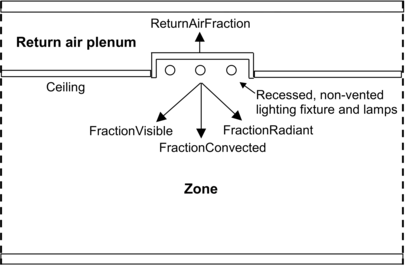
\includegraphics[width=0.9\textwidth, height=0.9\textheight, keepaspectratio=true]{media/image087.png}
\caption{Vertical section through a zone and its return air plenum showing recessed lighting (not to scale). The heat from lights is divided into four fractions, three of which --- ReturnAirFraction, FractionRadiant and FractionConvected --- depend on plenum air temperature. \protect \label{fig:vertical-section-through-a-zone-and-its}}
\end{figure}

An IDF example:

\begin{lstlisting}
Lights,
  RIGHT FORK Lights 1,  !- Name
  RIGHT FORK,           !- Zone Name
  Office Lighting,      !- SCHEDULE Name
  LightingLevel,        !- Design Level calculation method
  1039.706,             !- Lighting Level {W}
  0.0000000E+00,        !- Return Air Fraction
  0.4000000,            !- Fraction Radiant
  0.2000000,            !- Fraction Visible
  1.0,                  !- Fraction Replaceable
  GeneralLights;        !- End-Use Subcategory
\end{lstlisting}

Global Lights Object:

\begin{lstlisting}
ZoneList,AllOccupiedZones,SPACE1-1,SPACE2-1,SPACE3-1,SPACE4-1,SPACE5-1;

Lights,
  AllZones with Lights, !- Name
  AllOccupiedZones,     !- Zone or ZoneList Name
  LIGHTS-1,             !- Schedule Name
  Watts/Area,           !- Design Level Calculation Method
  ,                     !- Lighting Level {W}
  16,                   !- Watts per Zone Floor Area {W/m2}
  ,                     !- Watts per Person {W/person}
  0.2,                  !- Return Air Fraction
  0.59,                 !- Fraction Radiant
  0.2,                  !- Fraction Visible
  0,                    !- Fraction Replaceable
  GeneralLights;        !- End-Use Subcategory
\end{lstlisting}

\subsubsection{Outputs}\label{outputs-2-012}

If daylighting controls are operating in the zone, all of the Lights objects with a Fraction Replaceable greater than zero will be reduced by a multiplicative factor that accounts for how much the electric lighting is lowered due to daylighting.

Lights objects have output variables for individual objects and for zone totals.

\begin{itemize}
\item
  Zone,Average,Lights Electricity Rate {[}W{]}
\item
  Zone,Sum,Lights Radiant Heat Gain {[}J{]}
\item
  Zone,Average,Lights Radiant Heating Rate {[}W{]}
\item
  Zone,Sum,Lights Visible Radiation Heating Energy {[}J{]}
\item
  Zone,Average,Lights Visible Radiation Heating Rate {[}W{]}
\item
  Zone,Sum,Lights Convective Heating Energy {[}J{]}
\item
  Zone,Average,Lights Convective Heating Rate {[}W{]}
\item
  Zone,Sum,Lights Return Air Heating Energy {[}J{]}
\item
  Zone,Average,Lights Return Air Heating Rate {[}W{]}
\item
  Zone,Sum,Lights Total Heating Energy {[}J{]}
\item
  Zone,Average,Lights Total Heating Rate {[}W{]}
\item
  Zone,Sum,Lights Electricity Energy {[}J{]}
\item
  Zone,Average,Zone Lights Electricity Rate {[}W{]}
\item
  Zone,Sum,Zone Lights Radiant Heating Energy {[}J{]}
\item
  Zone,Average,Zone Lights Radiant Heating Rate {[}W{]}
\item
  Zone,Sum,Zone Lights Visible Radiation Heating Energy {[}J{]}
\item
  Zone,Average,Zone Lights Visible Radiation Heating Rate {[}W{]}
\item
  Zone,Sum,Zone Lights Convective Heating Energy {[}J{]}
\item
  Zone,Average,Zone Lights Convective Heating Rate {[}W{]}
\item
  Zone,Sum,Zone Lights Return Air Heating Energy {[}J{]}
\item
  Zone,Average,Zone Lights Return Air Heating Rate {[}W{]}
\item
  Zone,Sum,Zone Lights Total Heating Energy {[}J{]}
\item
  Zone,Average,Zone Lights Total Heating Rate {[}W{]}
\item
  Zone,Sum,Zone Lights Electricity Energy {[}J{]}
\end{itemize}

\paragraph{Lights Electricity Rate {[}W{]}}\label{lights-electric-power-w}

The electric power input for the lights.

\paragraph{Lights Radiant Heating Rate {[}W{]}}\label{lights-radiant-heating-rate-w}

\paragraph{Lights Radiant Heating Energy {[}J{]}}\label{lights-radiant-heating-energy-j}

The amount of heat gain from lights that is in the form of long-wave (thermal) radiation entering the zone. This heat is absorbed by the inside surfaces of the zone according to an area times long-wave absorptance weighting scheme.

\paragraph{Lights Visible Radiation Heating Rate {[}W{]}}\label{lights-visible-radiation-heating-rate-w}

\paragraph{Lights Visible Radiation Heating Energy {[}J{]}}\label{lights-visible-radiation-heating-energy-j}

The amount of heat gain from lights that is in the form of visible (short-wave) radiation entering the zone. This heat is absorbed by the inside surfaces of the zone according~ to an area times short-wave absorptance weighting scheme.

\paragraph{Lights Convective Heating Rate {[}W{]}}\label{lights-convective-heating-rate-w}

\paragraph{Lights Convective Heating Energy {[}J{]}}\label{lights-convective-heating-energy-j}

The amount of heat gain from lights that is convected to the zone air.

\paragraph{Lights Return Air Heating Rate {[}W{]}}\label{lights-return-air-heating-rate-w}

\paragraph{Lights Return Air Heating Energy {[}J{]}}\label{lights-return-air-heating-energy-j}

The amount of heat gain from lights that goes into the zone's return air (and, therefore, does not directly contribute to the zone load). If the zone has no return air system or the zone's air system is off, this heat will be added to the zone air.

\paragraph{Lights Total Heating Rate {[}W{]}}\label{lights-total-heating-rate-w}

\paragraph{Lights Total Heating Energy {[}J{]}}\label{lights-total-heating-energy-j}

The total heat gain from lights. It is the sum of the following four outputs, i.e., Total Heat Gain = Return Air Heat Gain + Radiant Heat Gain + Visible Heat Gain + Convective Heat Gain. It is also equal to the electrical input to the lights.

\paragraph{Lights Electricity Energy {[}J{]}}\label{lights-electric-energy-j}

The lighting electrical consumption including ballasts, if present. These will have the same value as Lights Total Heating Energy (above).

\paragraph{Zone Lights Electricity Rate {[}W{]}}\label{zone-lights-electric-power-w}

The electric power input for all lights in the zone.

\paragraph{Zone Lights Radiant Heating Rate {[}W{]}}\label{zone-lights-radiant-heating-rate-w}

\paragraph{Zone Lights Radiant Heating Energy {[}J{]}}\label{zone-lights-radiant-heating-energy-j}

The amount of heat gain from all lights in the zone that is in the form of long-wave (thermal) radiation entering the zone. This heat is absorbed by the inside surfaces of the zone according to an area times long-wave absorptance weighting scheme.

\paragraph{Zone Lights Visible Radiation Heating Rate {[}W{]}}\label{zone-lights-visible-radiation-heating-rate-w}

\paragraph{Zone Lights Visible Radiation Heating Energy {[}J{]}}\label{zone-lights-visible-radiation-heating-energy-j}

The amount of heat gain from all lights in the zone that is in the form of visible (short-wave) radiation entering the zone. This heat is absorbed by the inside surfaces of the zone according~ to an area times short-wave absorptance weighting scheme.

\paragraph{Zone Lights Convective Heating Rate {[}W{]}}\label{zone-lights-convective-heating-rate-w}

\paragraph{Zone Lights Convective Heating Energy {[}J{]}}\label{zone-lights-convective-heating-energy-j}

The amount of heat gain from all lights in the zone that is convected to the zone air.

\paragraph{Zone Lights Return Air Heating Rate {[}W{]}}\label{zone-lights-return-air-heating-rate-w}

\paragraph{Zone Lights Return Air Heating Energy {[}J{]}}\label{zone-lights-return-air-heating-energy-j}

The amount of heat gain from all lights in the zone that goes into the zone's return air (and, therefore, does not directly contribute to the zone load). If the zone has no return air system or the zone's air system is off, this heat will be added to the zone air.

\paragraph{Zone Lights Total Heating Rate {[}W{]}}\label{zone-lights-total-heating-rate-w}

\paragraph{Zone Lights Total Heating Energy {[}J{]}}\label{zone-lights-total-heating-energy-j}

The total heat gain from all lights in the zone. It is the sum of the following four outputs, i.e., Total Heat Gain = Return Air Heat Gain + Radiant Heat Gain + Visible Heat Gain + Convective Heat Gain. It is also equal to the electrical input to the lights.

\paragraph{Zone Lights Electricity Energy {[}J{]}}\label{zone-lights-electric-energy-j}

The lighting electrical consumption for all lights in the zone including ballasts, if present. This will have the same value as Zone Lights Total Heating Energy (above). However, this amount is also shown in the Electricity meters that are associated with the zone:

Electricity:Facility,

Electricity:Building,

Electricity:Zone:\textless{}Zone Name\textgreater{}.

In addition, depending on use, it will be shown in:

InteriorLights: Electricity and

InteriorLights:Electricity:Zone :\textless{}Zone Name\textgreater{}.

\subsubsection{Outputs}\label{outputs-3-010}

As described in the Lights Outputs, values for lights will show up on the following meters:

% table 15
\begin{longtable}[c]{>{\raggedright}p{3.0in}p{1.5in}p{1.5in}}
\caption{Distribution of Lights to Meters \label{table:distribution-of-lights-to-meters}} \tabularnewline
\toprule
Meter Name & Scope & Lights Specifics \tabularnewline
\midrule
\endfirsthead

\caption[]{Distribution of Lights to Meters} \tabularnewline
\toprule
Meter Name & Scope & Lights Specfics \tabularnewline
\midrule
\endhead

Electricity:Facility & Entire Facility & All \tabularnewline
Electricity:Building & All Zones & All \tabularnewline
Electricity:Zone: <Zone Name> & Specific Zone & All \tabularnewline
InteriorLights:Electricity & All Zones & Lights Use \tabularnewline
InteriorLights:Electricity:Zone: <Zone Name> & Specific Zone & Lights Use \tabularnewline
<End-Use Subcategory> :InteriorLights:Electricity & Specific Subcategory & Lights Use \tabularnewline
\bottomrule
\end{longtable}

\subsection{ElectricEquipment}\label{electricequipment}

The object models equipment in the zone which consumes electricity, such as computers, televisions, and cooking equipment, also known as ``plug loads.'' All of the energy consumed by the equipment becomes a heat gain in the zone or is lost (exhausted) as specified below.

\subsubsection{Inputs}\label{inputs-3-019}

\paragraph{Field: Name}\label{field-name-3-017}

The name of the ElectricEquipment object.

\paragraph{Field: Zone or ZoneList Name}\label{field-zone-or-zonelist-name-2}

This field is the name of the zone (ref: Zone) or \hyperref[zonelist]{ZoneList} (ref: \hyperref[zonelist]{ZoneList}) and attaches a particular electric equipment statement to a thermal zone or set of thermal zones in the building. When the \hyperref[zonelist]{ZoneList} option is used then this electric equipment definition is applied to each of the zones in the zone list effecting a global definition for the amount of electric wattage in the zone. The Zonelist option can be used effectively with the watts/area and watts/person options of the Design Level Calculation Method.

The name of the actual electric equipment object becomes \textless{}Zone Name\textgreater{} \textless{}ElectricEquipment Object Name\textgreater{} and should be less than the standard length (100 characters) for a name field. If it is greater than this standard length, it may be difficult to specify in output reporting as it will be truncated. A warning will be shown if the generated name is greater than 100 characters. If it duplicates another such concatenated name, there will be a severe error and terminate the run.

\paragraph{Field: Schedule Name}\label{field-schedule-name-1-001}

This field is the name of the schedule that modifies the design level parameter for electric equipment (see Design Level Calculation Method field and related subsequent fields). The schedule values can be any positive number. The actual electrical input for equipment in a zone as defined by this statement is the product of the design level field and the value of the schedule specified by name in this field.

\paragraph{Field: Design Level Calculation Method}\label{field-design-level-calculation-method-1}

This field is a key/choice field that tells which of the next three fields are filled and is descriptive of the method for calculating the nominal electric equipment level in the Zone. The key/choices are:

\begin{itemize}
\tightlist
\item
  EquipmentLevel
\end{itemize}

With this choice, the method used will be a straight insertion of the electric equipment level (Watts) for the Zone.~ (The Design Level field should be filled.)

\begin{itemize}
\tightlist
\item
  Watts/Area
\end{itemize}

With this choice, the method used will be a factor per floor area of the zone. (The Watts per Zone Floor Area field should be filled).

\begin{itemize}
\tightlist
\item
  Watts/Person
\end{itemize}

With this choice, the method used will be a factor of equipment level (watts) per person. (The Watts per Person field should be filled).

\paragraph{Field: Design Level}\label{field-design-level-000}

This field (in Watts) is typically used to represent the maximum electrical input to equipment in a zone that is then multiplied by a schedule fraction (see previous field). In EnergyPlus, this is slightly more flexible in that the electric equipment design level could be a ``diversity factor'' applied to a schedule of real numbers. Note that while the schedule value can vary from hour to hour, the design level field is constant for all simulation environments.

\paragraph{Field: Watts per Zone Floor Area}\label{field-watts-per-zone-floor-area-1}

This factor (watts/m\(^{2}\)) is used, along with the Zone Area to determine the maximum equipment level as described in the Design Level field. The choice from the method field should be ``Watts/Area''.

\paragraph{Field: Watts per Person}\label{field-watts-per-person-1}

This factor (watts/person) is used, along with the number of occupants (people) to determine the maximum equipment level as described in the Design Level field. The choice from the method field should be ``Watts/Person''.

\paragraph{Heat Gains from Electric Equipment:}\label{heat-gains-from-electric-equipment}

The electrical input to the equipment ultimately appears as heat that contributes to zone loads. In EnergyPlus this heat is divided into four different fractions. Three of these are given by the input fields Fraction Latent, Fraction Radiant and Fraction Lost. A fourth, defined as the fraction of the heat from electric equipment convected to the zone air, is calculated by the program as:

\begin{equation}
  f_{\rm{convected}} = 1.0 - (\rm{Fraction Latent} + \rm{Fraction Radiant} + \rm{Fraction Lost})
\end{equation}

You will get an error message if Fraction Latent + Fraction Radiant + Fraction Lost exceeds 1.0.

\paragraph{Field: Fraction Latent}\label{field-fraction-latent}

This field is a decimal number between 0.0 and 1.0 and is used to characterize the amount of latent heat given off by electric equipment in a zone. The number specified in this field will be multiplied by the total energy consumed by electric equipment to give the amount of latent energy produced by the electric equipment. This energy affects the moisture balance within the zone.

\paragraph{Field: Fraction Radiant}\label{field-fraction-radiant-2}

This field is a decimal number between 0.0 and 1.0 and is used to characterize the amount of long-wave radiant heat being given off by electric equipment in a zone. The number specified in this field will be multiplied by the total energy consumed by electric equipment to give the amount of long wavelength radiation gain from electric equipment in a zone.

\paragraph{Field: Fraction Lost}\label{field-fraction-lost}

This field is a decimal number between 0.0 and 1.0 and is used to characterize the amount of ``lost'' heat being given off by electric equipment in a zone. The number specified in this field will be multiplied by the total energy consumed by electric equipment to give the amount of heat which is ``lost'' and does not impact the zone energy balances. This might correspond to electrical energy converted to mechanical work or heat that is vented to the atmosphere.

\paragraph{Field: End-Use Subcategory}\label{field-end-use-subcategory-1-001}

Allows you to specify a user-defined end-use subcategory, e.g., ``Computers'', ``Copy Machines'', etc. A new meter for reporting is created for each unique subcategory~ (ref: \hyperref[outputmeter-and-outputmetermeterfileonly]{Output:Meter} objects). Subcategories are also reported in the ABUPS table. If this field is omitted or blank, the equipment will be assigned to the ``General'' end-use subcategory. Any text may be used here to categorize the end-uses in the ABUPS End Uses by Subcategory table and the LEED Summary table EAp2-4/5. Performance Rating Method Compliance.


An IDF example:

\begin{lstlisting}
ElectricEquipment,
  DORM ROOMS AND COMMON AREAS ElecEq 1, !- Name
  DORM ROOMS AND COMMON AREAS,          !- Zone Name
  Residence Equipment,                  !- SCHEDULE Name
  EquipmentLevel,                       !- Design Level calculation method
  9210.921,                             !- Design Level {W}
  ,                                     !- Watts per Zone Floor Area {watts/m2}
  ,                                     !- Watts per Person {watts/person}
  0.0000000E+00,                        !- Fraction Latent
  0.3000000,                            !- Fraction Radiant
  0.0000000E+00,                        !- Fraction Lost
  Computers;                            !- End-use Subcategory
\end{lstlisting}

Global ElectricEquipment example:

\begin{lstlisting}
ZoneList,AllOccupiedZones,SPACE1-1,SPACE2-1,SPACE3-1,SPACE4-1,SPACE5-1;

ElectricEquipment,
  AllZones with Electric Equipment,     !- Name
  AllOccupiedZones,                     !- Zone or ZoneList Name
  EQUIP-1,                              !- Schedule Name
  Watts/Person,                         !- Design Level Calculation Method
  ,                                     !- Design Level {W}
  ,                                     !- Watts per Zone Floor Area {W/m2}
  96,                                   !- Watts per Person {W/person}
  0,                                    !- Fraction Latent
  0.3,                                  !- Fraction Radiant
  0;                                    !- Fraction Lost
\end{lstlisting}

\subsection{GasEquipment}\label{gasequipment}

The object models equipment in the zone which consumes natural gas, such as cooking equipment or a gas fireplace. All of the energy consumed by the equipment becomes a heat gain in the zone or is lost (exhausted) as specified below.

\subsubsection{Inputs}\label{inputs-4-017}

\paragraph{Field: Name}\label{field-name-4-014}

The name of the GasEquipment object.

\paragraph{Field: Zone or ZoneList Name}\label{field-zone-or-zonelist-name-3}

This field is the name of the thermal zone (ref: Zone) or \hyperref[zonelist]{ZoneList} (ref: \hyperref[zonelist]{ZoneList}) and attaches a particular gas equipment statement to a thermal zone or set of thermal zones in the building. When the \hyperref[zonelist]{ZoneList} option is used then this gas equipment definition is applied to each of the zones in the zone list effecting a global definition for the amount of gas in the zone. The Zonelist option can be used effectively with the watts/area and watts/person options of the Design Level Calculation Method.

The name of the actual gas equipment object becomes \textless{}Zone Name\textgreater{} \textless{}GasEquipment Object Name\textgreater{} and should be less than the standard length (100 characters) for a name field. If it is greater than this standard length, it may be difficult to specify in output reporting as it will be truncated. A warning will be shown if the generated name is greater than 100 characters. If it duplicates another such concatenated name, there will be a severe error and terminate the run.

\paragraph{Field: Schedule Name}\label{field-schedule-name-2-001}

This field is the name of the schedule that modifies the design level parameter for gas equipment (see Design Level Calculation Method field and related subsequent fields). The schedule values can be any positive number. The actual energy input for gas equipment in a zone as defined by this statement is the product of the design level field and the value of the schedule specified by name in this field.

\paragraph{Field: Design Level Calculation Method}\label{field-design-level-calculation-method-2}

This field is a key/choice field that tells which of the next three fields are filled and is descriptive of the method for calculating the nominal gas equipment level in the Zone. The key/choices are:

\begin{itemize}
\tightlist
\item
  EquipmentLevel
\end{itemize}

With this choice, the method used will be a straight insertion of the gas equipment level (Watts) for the Zone.~ (The Design Level field should be filled.)

\begin{itemize}
\tightlist
\item
  Watts/Area or Power/Area
\end{itemize}

With this choice, the method used will be a factor per floor area of the zone. (The Power per Zone Floor Area field should be filled).

\begin{itemize}
\tightlist
\item
  Watts/Person or Power/Person
\end{itemize}

With this choice, the method used will be a factor of equipment level (watts) per person. (The Power per Person field should be filled).

\paragraph{Field: Design Level}\label{field-design-level-1-000}

This field (in Watts) is typically used to represent the maximum energy input to gas equipment in a zone that is then multiplied by a schedule fraction (see previous field). In EnergyPlus, this is slightly more flexible in that the gas equipment design level could be a ``diversity factor'' applied to a schedule of real numbers. Note that while the schedule value can vary from hour to hour, the design level field is constant for all simulation environments.

\paragraph{Field: Power per Zone Floor Area}\label{field-power-per-zone-floor-area}

This factor (watts/m\(^{2}\)) is used, along with the Zone Area to determine the maximum equipment level as described in the Design Level field. The choice from the method field should be ``\textbf{Watts/Area}'' or ``\textbf{Power/Area}''.

\paragraph{Field: Power per Person}\label{field-power-per-person}

This factor (watts/person) is used, along with the number of occupants (people) to determine the maximum equipment level as described in the Design Level field. The choice from the method field should be ``\textbf{Watts/Person}'' or ``\textbf{Power/Person}''.

\paragraph{Heat Gains from Gas Equipment:}\label{heat-gains-from-gas-equipment}

The fuel input to the equipment ultimately appears as heat that contributes to zone loads. In EnergyPlus this heat is divided into four different fractions. Three of these are given by the input fields Fraction Latent, Fraction Radiant and Fraction Lost. A fourth, defined as the fraction of the heat from gas equipment convected to the zone air, is calculated by the program as:

\begin{equation}
  f_{convected} = 1.0 - (\rm{Fraction Latent} + \rm{Fraction Radiant} + \rm{Fraction Lost})
\end{equation}

You will get an error message if Fraction Latent + Fraction Radiant + Fraction Lost exceeds 1.0.

\paragraph{Field: Fraction Latent}\label{field-fraction-latent-1}

This field is a decimal number between 0.0 and 1.0 and is used to characterize the amount of latent heat given off by gas equipment in a zone. The number specified in this field will be multiplied by the total energy consumed by gas equipment to give the amount of latent energy produced by the gas equipment. This energy affects the moisture balance within the zone.

\paragraph{Field: Fraction Radiant}\label{field-fraction-radiant-3}

This field is a decimal number between 0.0 and 1.0 and is used to characterize the amount of long-wave radiant heat being given off by gas equipment in a zone. The number specified in this field will be multiplied by the total energy consumed by gas equipment to give the amount of long wavelength radiation gain from gas equipment in a zone.

\paragraph{Field: Fraction Lost}\label{field-fraction-lost-1}

This field is a decimal number between 0.0 and 1.0 and is used to characterize the amount of ``lost'' heat being given off by gas equipment in a zone. The number specified in this field will be multiplied by the total energy consumed by gas equipment to give the amount of heat which is ``lost'' and does not impact the zone energy balances. This might correspond to input energy converted to mechanical work or heat that is vented to the atmosphere.

\paragraph{Field: Carbon Dioxide Generation Rate}\label{field-carbon-dioxide-generation-rate-1}

This numeric input field specifies carbon dioxide generation rate with units of m3/s-W. The default value of 0.0 assumes the equipment is fully vented to outdoors. In the absence of better information, the user might consider using a value of 3.45E-8 m3/s-W which assumes the equipment is not vented to outdoors. This value is converted from natural gas CO\(_{2}\) emission rate at 11.7 lbs CO\(_{2}\) per therm. The CO\(_{2}\) emission rate is provided by U.S. Energy Information Administration, ``Frequently Asked Questions - Environment, Questions About Environmental Emissions'', \url{http://tonto.eia.doe.gov/ask/environment_faqs.asp#CO2_quantity}, January 2010. The maximum value for this input field is 3.45E-7 m3/s-W.

\paragraph{Field: End-Use Subcategory}\label{field-end-use-subcategory-2-001}

Allows you to specify a user-defined end-use subcategory, e.g., ``Cooking'', ``Clothes Drying'', etc. A new meter for reporting is created for each unique subcategory~ (ref: \hyperref[outputmeter-and-outputmetermeterfileonly]{Output:Meter} objects). Subcategories are also reported in the ABUPS table. If this field is omitted or blank, the equipment will be assigned to the ``General'' end-use subcategory. Any text may be used here to categorize the end-uses in the ABUPS End Uses by Subcategory table and the LEED Summary table EAp2-4/5 Performance Rating Method Compliance.

An IDF example:

\begin{lstlisting}
GasEquipment,
  DORM ROOMS AND COMMON AREAS GasEq 1,  !- Name
  DORM ROOMS AND COMMON AREAS,          !- Zone Name
  Gas Eq Sch,                           !-Schedule Name
  EquipmentLevel,                       !- Design Level Calculation Method
  29287.51,                             !- Design Level {W}
  ,                                     !- Power per Zone Floor Area {W/m2}
  ,                                     !- Power per Person {W/Person}
  0,                                    !- Fraction Latent
  0.3,                                  !- Fraction Radiant
  0,                                    !- Fraction Lost
  0,                                    !- Carbon Dioxide Generation Rate {m3/s-W}
  Cooking;                              !- End-Use Subcategory
\end{lstlisting}

Global Gas Equipment example:

\begin{lstlisting}
ZoneList,OfficeZones,Left Fork, Middle Fork, Right Fork;

GasEquipment,
  Office Zones with Gas,                !- Name
  OfficeZones,                          !- Zone Name
  Gas Eq Sch,                           !- Schedule Name
  Watts/Area,                           !- Design Level Calculation Method
  ,                                     !- Design Level {W}
  197,                                  !- Power per Zone Floor Area {W/m2}
  ,                                     !- Power per Person {W/Person}
  0.0000000E+00,                        !- Fraction Latent
  0.3000000,                            !- Fraction Radiant
  0.0000000E+00;                        !- Fraction Lost
\end{lstlisting}

\subsection{HotWaterEquipment}\label{hotwaterequipment}

The object models hot water equipment in the zone which consumes district heating, such as cooking equipment or process loads. All of the energy consumed by the equipment becomes a heat gain in the zone or is lost (exhausted) as specified below. This object consumes district heating energy directly and does not cause a load on a hot water plant loop or water heater. For domestic hot water uses, such as sinks and showers, see \hyperref[wateruseequipment]{WaterUse:Equipment}.

\subsubsection{Inputs}\label{inputs-5-015}

\paragraph{Field: Name}\label{field-name-5-011}

The name of the HotWaterEquipment object.

\paragraph{Field: Zone or ZoneList Name}\label{field-zone-or-zonelist-name-4}

This field is the name of the thermal zone (ref: Zone) or \hyperref[zonelist]{ZoneList} (ref: \hyperref[zonelist]{ZoneList}) and attaches a particular hot water equipment statement to a thermal zone or set of thermal zones in the building. When the \hyperref[zonelist]{ZoneList} option is used then this hot water equipment definition is applied to each of the zones in the zone list effecting a global definition for the amount of hot water in the zone. The Zonelist option can be used effectively with the watts/area and watts/person options of the Design Level Calculation Method.

The name of the actual hot water equipment object becomes \textless{}Zone Name\textgreater{} \textless{}HotWaterEquipment Object Name\textgreater{} and should be less than the standard length (100 characters) for a name field. If it is greater than this standard length, it may be difficult to specify in output reporting as it will be truncated. A warning will be shown if the generated name is greater than 100 characters. If it duplicates another such concatenated name, there will be a severe error and terminate the run.

\paragraph{Field: Schedule Name}\label{field-schedule-name-3-000}

This field is the name of the schedule that modifies the design level parameter for hot water equipment (see Design Level Calculation Method field and related subsequent fields). The schedule values can be any positive number. The actual energy input for hot water equipment in a zone as defined by this statement is the product of the design level field and the value of the schedule specified by name in this field.

\paragraph{Field: Design Level Calculation Method}\label{field-design-level-calculation-method-3}

This field is a key/choice field that tells which of the next three fields are filled and is descriptive of the method for calculating the nominal hot water equipment level in the Zone. The key/choices are:

\begin{itemize}
\tightlist
\item
  EquipmentLevel
\end{itemize}

With this choice, the method used will be a straight insertion of the hot water equipment level (Watts) for the Zone.~ (The Design Level field should be filled.)

\begin{itemize}
\tightlist
\item
  Watts/Area or Power/Area
\end{itemize}

With this choice, the method used will be a factor per floor area of the zone. (The Power per Zone Floor Area field should be filled).

\begin{itemize}
\tightlist
\item
  Watts/Person or Power/Person
\end{itemize}

With this choice, the method used will be a factor of equipment level (watts) per person. (The Power per Person field should be filled).

\paragraph{Field: Design Level}\label{field-design-level-2-000}

This field (in Watts) is typically used to represent the maximum energy input to hot water equipment in a zone that is then multiplied by a schedule fraction (see previous field). In EnergyPlus, this is slightly more flexible in that the hot water equipment design level could be a ``diversity factor'' applied to a schedule of real numbers. Note that while the schedule value can vary from hour to hour, the design level field is constant for all simulation environments.

\paragraph{Field: Power per Zone Floor Area}\label{field-power-per-zone-floor-area-1}

This factor (watts/m\(^{2}\)) is used, along with the Zone Area to determine the maximum equipment level as described in the Design Level field. The choice from the method field should be ``\textbf{Watts/Area}'' or ``\textbf{Power/Area}''.

\paragraph{Field: Power per Person}\label{field-power-per-person-1}

This factor (watts/person) is used, along with the number of occupants (people) to determine the maximum equipment level as described in the Design Level field. The choice from the method field should be ``\textbf{Watts/Person}'' or ``\textbf{Power/Person}''.

\paragraph{Heat Gains from Hot Water Equipment:}\label{heat-gains-from-hot-water-equipment}

The fuel input to the equipment ultimately appears as heat that contributes to zone loads. In EnergyPlus this heat is divided into four different fractions. Three of these are given by the input fields Fraction Latent, Fraction Radiant and Fraction Lost. A fourth, defined as the fraction of the heat from hot water equipment convected to the zone air, is calculated by the program as:

\begin{equation}
  f_{\rm{convected}} = 1.0 - (\rm{Fraction Latent} + \rm{Fraction Radiant} + \rm{Fraction Lost})
\end{equation}

You will get an error message if Fraction Latent + Fraction Radiant + Fraction Lost exceeds 1.0.

\paragraph{Field: Fraction Latent}\label{field-fraction-latent-2}

This field is a decimal number between 0.0 and 1.0 and is used to characterize the amount of latent heat given off by hot water equipment in a zone. The number specified in this field will be multiplied by the total energy consumed by hot water equipment to give the amount of latent energy produced by the hot water equipment. This energy affects the moisture balance within the zone.

\paragraph{Field: Fraction Radiant}\label{field-fraction-radiant-4}

This field is a decimal number between 0.0 and 1.0 and is used to characterize the amount of long-wave radiant heat being given off by hot water equipment in a zone. The number specified in this field will be multiplied by the total energy consumed by hot water equipment to give the amount of long wavelength radiation gain from hot water equipment in a zone.

\paragraph{Field: Fraction Lost}\label{field-fraction-lost-2}

This field is a decimal number between 0.0 and 1.0 and is used to characterize the amount of ``lost'' heat being given off by hot water equipment in a zone. The number specified in this field will be multiplied by the total energy consumed by hot water equipment to give the amount of heat which is ``lost'' and does not impact the zone energy balances. This might correspond to input energy converted to mechanical work or heat that is vented to the atmosphere.

\paragraph{Field: End-Use Subcategory}\label{field-end-use-subcategory-3-000}

Allows you to specify a user-defined end-use subcategory, e.g., ``Cooking'', ``Clothes Drying'', etc. A new meter for reporting is created for each unique subcategory~ (ref: \hyperref[outputmeter-and-outputmetermeterfileonly]{Output:Meter} obejct). Subcategories are also reported in the ABUPS table. If this field is omitted or blank, the equipment will be assigned to the ``General'' end-use subcategory. Any text may be used here to categorize the end-uses in the ABUPS End Uses by Subcategory table and the LEED Summary table EAp2-4/5 Performance Rating Method Compliance.

IDF Examples:

\begin{lstlisting}
HotWaterEquipment,
  SPACE2-1 HWEq 1,    !- Name
  SPACE2-1,           !- Zone Name
  EQUIP-1,            !- SCHEDULE Name
  EquipmentLevel,     !- Design Level calculation method
  300,                !- Design Level {W}
  ,                   !- Power per Zone Floor Area {watts/m2}
  ,                   !- Power per Person {watts/person}
  0.2,                !- Fraction Latent
  0.1,                !- Fraction Radiant
  0.5,                !- Fraction Lost
  Dishwashing;        !- End-Use Subcategory
\end{lstlisting}

Global Hot Water Equipment example:

\begin{lstlisting}
ZoneList,OfficeZones,Left Fork, Middle Fork, Right Fork;

HotWaterEquipment,
  Office Zones with HoWater Equipment,!- Name
  OfficeZones,                        !- Zone Name
  HotWater Eq Sch,                    !- Schedule Name
  Watts/Area,                         !- Design Level Calculation Method
  ,                                   !- Design Level {W}
  50,                                 !- Power per Zone Floor Area {W/m2}
  ,                                   !- Power per Person {W/Person}
  0.0000000E+00,                      !- Fraction Latent
  0.3000000,                          !- Fraction Radiant
  0.0000000E+00;                      !- Fraction Lost
\end{lstlisting}

\subsection{SteamEquipment}\label{steamequipment}

The object models steam equipment in the zone which consumes district heating, such as cooking equipment or process loads. All of the energy consumed by the equipment becomes a heat gain in the zone or is lost (exhausted) as specified below. This object consumes district heating energy directly and does not cause a load on a steam plant loop.

\subsubsection{Inputs}\label{inputs-6-012}

\paragraph{Field: Name}\label{field-name-6-009}

The name of the SteamEquipment object.

\paragraph{Field: Zone or ZoneList Name}\label{field-zone-or-zonelist-name-5}

This field is the name of the thermal zone (ref: Zone) and attaches a particular steam equipment statement to a thermal zone or set of thermal zones in the building. When the \hyperref[zonelist]{ZoneList} option is used then this steam equipment definition is applied to each of the zones in the zone list effecting a global definition for the amount of steam in the zone. This option can be used effectively with the watts/area and watts/person options of the Design Level Calculation Method.

\paragraph{Field: Schedule Name}\label{field-schedule-name-4-000}

This field is the name of the schedule that modifies the design level parameter for steam equipment (see Design Level Calculation Method field and related subsequent fields). The schedule values can be any positive number. The actual energy input for steam equipment in a zone as defined by this statement is the product of the design level field and the value of the schedule specified by name in this field.

\paragraph{Field: Design Level Calculation Method}\label{field-design-level-calculation-method-4}

This field is a key/choice field that tells which of the next three fields are filled and is descriptive of the method for calculating the nominal steam equipment level in the Zone. The key/choices are:

\begin{itemize}
\tightlist
\item
  EquipmentLevel
\end{itemize}

With this choice, the method used will be a straight insertion of the steam equipment level (Watts) for the Zone.~ (The Design Level field should be filled.)

\begin{itemize}
\tightlist
\item
  Watts/Area or Power/Area
\end{itemize}

With this choice, the method used will be a factor per floor area of the zone. (The Power per Zone Floor Area field should be filled).

\begin{itemize}
\tightlist
\item
  Watts/Person or Power/Person
\end{itemize}

With this choice, the method used will be a factor of equipment level (watts) per person. (The Power per Person field should be filled).

\paragraph{Field: Design Level}\label{field-design-level-3}

This field (in Watts) is typically used to represent the maximum energy input to steam equipment in a zone that is then multiplied by a schedule fraction (see previous field). In EnergyPlus, this is slightly more flexible in that the steam equipment design level could be a ``diversity factor'' applied to a schedule of real numbers. Note that while the schedule value can vary from hour to hour, the design level field is constant for all simulation environments.

\paragraph{Field: Power per Zone Floor Area}\label{field-power-per-zone-floor-area-2}

This factor (watts/m\(^{2}\)) is used, along with the Zone Area to determine the maximum equipment level as described in the Design Level field. The choice from the method field should be ``\textbf{Watts/Area}'' or ``\textbf{Power/Area}''.

\paragraph{Field: Power per Person}\label{field-power-per-person-2}

This factor (watts/person) is used, along with the number of occupants (people) to determine the maximum equipment level as described in the Design Level field. The choice from the method field should be ``\textbf{Watts/Person}'' or ``\textbf{Power/Person}''.

\paragraph{Heat Gains from Steam Equipment:}\label{heat-gains-from-steam-equipment}

The fuel input to the equipment ultimately appears as heat that contributes to zone loads. In EnergyPlus this heat is divided into four different fractions. Three of these are given by the input fields Fraction Latent, Fraction Radiant and Fraction Lost. A fourth, defined as the fraction of the heat from steam equipment convected to the zone air, is calculated by the program as:

\begin{equation}
  f_{\rm{convected}} = 1.0 - (\rm{Fraction Latent} + \rm{Fraction Radiant} + \rm{Fraction Lost})
\end{equation}

You will get an error message if Fraction Latent + Fraction Radiant + Fraction Lost exceeds 1.0.

\paragraph{Field: Fraction Latent}\label{field-fraction-latent-3}

This field is a decimal number between 0.0 and 1.0 and is used to characterize the amount of latent heat given off by steam equipment in a zone. The number specified in this field will be multiplied by the total energy consumed by steam equipment to give the amount of latent energy produced by the steam equipment. This energy affects the moisture balance within the zone.

\paragraph{Field: Fraction Radiant}\label{field-fraction-radiant-5}

This field is a decimal number between 0.0 and 1.0 and is used to characterize the amount of long-wave radiant heat being given off by steam equipment in a zone. The number specified in this field will be multiplied by the total energy consumed by steam equipment to give the amount of long wavelength radiation gain from steam equipment in a zone.

\paragraph{Field: Fraction Lost}\label{field-fraction-lost-3}

This field is a decimal number between 0.0 and 1.0 and is used to characterize the amount of ``lost'' heat being given off by steam equipment in a zone. The number specified in this field will be multiplied by the total energy consumed by steam equipment to give the amount of heat which is ``lost'' and does not impact the zone energy balances. This might correspond to input energy converted to mechanical work or heat that is vented to the atmosphere.

\paragraph{Field: End-Use Subcategory}\label{field-end-use-subcategory-4-000}

Allows you to specify a user-defined end-use subcategory, e.g., ``Cooking'', ``Clothes Drying'', etc. A new meter for reporting is created for each unique subcategory~ (ref: \hyperref[outputmeter-and-outputmetermeterfileonly]{Output:Meter} objects). Subcategories are also reported in the ABUPS table. If this field is omitted or blank, the equipment will be assigned to the ``General'' end-use subcategory. Any text may be used here to categorize the end-uses in the ABUPS End Uses by Subcategory table and the LEED Summary table EAp2-4/5 Performance Rating Method Compliance.

IDF Examples:

\begin{lstlisting}

SteamEquipment,
  SPACE4-1 ElecEq 1, !- Name
  SPACE4-1,          !- Zone Name
  EQUIP-1,           !- SCHEDULE Name
  EquipmentLevel,    !- Design Level calculation method
  1050,              !- Design Level {W}
  ,                  !- Power per Zone Floor Area {watts/m2}
  ,                  !- Power per Person {watts/person}
  0.5,               !- Fraction Latent
  0.3,               !- Fraction Radiant
  0,                 !- Fraction Lost
  Laundry;           !- End-Use Subcategory
\end{lstlisting}

\subsection{SwimmingPool:Indoor}\label{swimmingpoolindoor}

The Indoor Swimming Pool object is used to describe the indoor swimming pools that are exposed to the internal environment. There are several rules that should be noted regarding the specification of an indoor pool in EnergyPlus. First, the pool is linked to a surface that must be a floor. The pool is assumed to cover the entire floor to which it is linked. If the pool only covers part of the floor in the actual building, then the user must break the floor up into multiple sections.

As pools attempt to achieve a particular water temperature and have a variety of heat losses, heating equipment is necessary to maintain the proper setpoint temperature. In EnergyPlus, the pool itself becomes part of the demand side of a plant loop with heating equipment on the supply side providing whatever heating is needed to maintain the desired temperature. This heating equipment as well as the loop connections must be entered separately and the input shown in this section only details what is needed to specify the pool itself.

There are a variety of rules that limit the application of indoor swimming pools in EnergyPlus.  The following are a list of these rules:

\begin{itemize}
  \item The pool must reference a valid surface in the input file.  This surface must be a floor and cannot be other surface types like ceilings, walls, windows, etc.
  \item The pool cannot refer to a surface that is also a radiant system, ventilated slab, or another pool.
  \item The surface that the pool references must be modeled using conduction transfer functions (CTF).
  \item The pool cannot utilize movable insulation or have a heat source or sink associated with it (something used to model low temperature radiant systems).
\end{itemize}

The following information is useful for defining and modeling an indoor pool in EnergyPlus. For more information on the algorithm used for this model or details on some of the input parameters, please reference the indoor pool section of the EnergyPlus Engineering Reference document.

\subsubsection{Inputs}\label{inputs-7-012}

\paragraph{Field: Name}\label{field-name-7-008}

This is a unique name associated with the indoor swimming pool.

\paragraph{Field: Surface Name}\label{field-surface-name-1-000}

This is the name of the surface (floor) where the pool is located. Pools are not allowed on any surfaces other than a floor.  For more rules on surfaces that can be used for pools, please see the information in this section on indoor pools above.

\paragraph{Field: Average Depth}\label{field-average-depth}

This field is the average depth of the pool in meters. If the pool has variable depth, the average depth should be specified to achieve the proper volume of water in the pool.

\paragraph{Field: Activity Factor Schedule Name}\label{field-activity-factor-schedule-name}

This field references a schedule that contains values for pool activity. This parameter can be varied using the schedule named here, and it has an impact on the amount of evaporation that will take place from the pool to the surrounding zone air. For example values of the activity factor and what impact it will have on the evaporation of water from the pool, please refer to the Indoor Swimming Pool section of the EnergyPlus Engineering Reference document. If left blank, the activity factor will be assumed to be unity. Note that the activity factor should not be set equal to an occupancy schedule since an activity factor of zero means that no evaporation will take place from the pool.

\paragraph{Field: Make-up Water Supply Schedule Name}\label{field-make-up-water-supply-schedule-name}

The scheduled named by this field establishes a cold water temperature {[}C{]} for the water that replaces the water which is lost from the pool due to evaporation. If blank, water temperatures are calculated by the \hyperref[sitewatermainstemperature]{Site:WaterMainsTemperature} object. This field (even if blank) overrides the Cold Water Supply Temperature Schedule in all of the listed \hyperref[wateruseequipment]{WaterUse:Equipment} objects.

\paragraph{Field: Cover Schedule Name}\label{field-cover-schedule-name}

This schedule defines when the pool water cover is available and affects the evaporation, convection, and radiation rate calculations. A schedule value of 0.0 means that the pool is not covered. A schedule value of 1.0 means the pool is 100\% covered. The pool may be fully covered, fully open (uncovered), or partially covered (a value between 0.0 and 1.0). The user also has the option to control the evaporation, convection, short-wavelength radiation, and long-wavelength radiation factors when the pool is covered. These terms are discussed in the next four fields.

\paragraph{Field: Cover Evaporation Factor}\label{field-cover-evaporation-factor}

This input field can optionally be used to modify the pool evaporation rate and is used in conjunction with the pool cover factor defined by the Pool Cover Schedule field (see above). The value for this parameter can normally range from 0.0 to 1.0, where 1 means that the pool cover completely eliminates evaporation from the pool surface, 0 means the pool cover has no effect on evaporation, and fractions in between 0 and 1 result in a fractional reduction in evaporation by the pool cover. So, if this parameter is 0.5 and the pool is 50\% covered, the overall reduction in evaporation from a fully uncovered pool is 25\% or 0.25.

\paragraph{Field: Cover Convection Factor}\label{field-cover-convection-factor}

This input field can optionally be used to modify the pool convection rate and is used in conjunction with the pool cover factor defined by the Pool Cover Schedule field (see above). The value for this parameter can normally range from 0.0 to 1.0, where 1 means that the pool cover completely eliminates convection from the pool surface, 0 means the pool cover has no effect on convection, and fractions in between 0 and 1 result in a fractional reduction in convection by the pool cover. So, if this parameter is 0.5 and the pool is 50\% covered, the overall reduction in convection from a fully uncovered pool is 25\% or 0.25.

\paragraph{Field: Cover Short-Wavelength Radiation Factor}\label{field-cover-short-wavelength-radiation-factor}

This input field can optionally be used to modify the pool short-wavelength radiation rate and is used in conjunction with the pool cover factor defined by the Pool Cover Schedule field (see above). The value for this parameter can normally range from 0.0 to 1.0, where 1 means that the pool cover completely eliminates short-wavelength radiation from the pool surface, 0 means the pool cover has no effect on short-wavelength radiation, and fractions in between 0 and 1 result in a fractional reduction in short-wavelength radiation by the pool cover. So, if this parameter is 0.5 and the pool is 50\% covered, the overall reduction in short-wavelength radiation from a fully uncovered pool is 25\% or 0.25. Note that with radiation terms that whatever portion of the short-wavelength radiation is blocked by the cover is transferred via convection to the surrounding zone air.

\paragraph{Field: Cover Long-Wavelength Radiation Factor}\label{field-cover-long-wavelength-radiation-factor}

This input field can optionally be used to modify the pool long-wavelength radiation rate and is used in conjunction with the pool cover factor defined by the Pool Cover Schedule field (see above). The value for this parameter can normally range from 0.0 to 1.0, where 1 means that the pool cover completely eliminates long-wavelength radiation from the pool surface, 0 means the pool cover has no effect on long-wavelength radiation, and fractions in between 0 and 1 result in a fractional reduction in long-wavelength radiation by the pool cover. So, if this parameter is 0.5 and the pool is 50\% covered, the overall reduction in long-wavelength radiation from a fully uncovered pool is 25\% or 0.25. Note that with radiation terms that whatever portion of the long-wavelength radiation is blocked by the cover is transferred via convection to the surrounding zone air.

\paragraph{Field: Pool Water Inlet Node}\label{field-pool-water-inlet-node}

This input is the name of the node on the demand side of a plant loop that leads into the pool. From the standpoint of an EnergyPlus input file, the pool sits on a plant demand loop, and the pump and heater reside on the plant supply loop. The pool heater and pump must be defined by other existing EnergyPlus input.

\paragraph{Field: Pool Water Outlet Node}\label{field-pool-water-outlet-node}

This input is the name of the node on the demand side of a plant loop that leads out of the pool. From the standpoint of an EnergyPlus input file, the pool sits on a plant demand loop, and the pump and heater reside on the plant supply loop. The pool heater and pump must be defined by other existing EnergyPlus input.

\paragraph{Field: Pool Water Maximum Flow Rate}\label{field-pool-water-maximum-flow-rate}

This input is the maximum water volumetric flow rate in m3/s going between the pool and the water heating equipment. This along with the pool setpoint temperature and the heating plant equipment outlet temperature will establish the maximum heat addition to the pool. This flow rate to the pool will be varied in an attempt to reach the desired pool water setpoint temperature (see Setpoint Temperature Schedule below).

\paragraph{Field: Pool Miscellaneous Equipment Power}\label{field-pool-miscellaneous-equipment-power}

This input defines the power consumption rate of miscellaneous equipment such as the filtering and chlorination technology associated with the pool. The units for this input are in power consumption per flow rate of water through the pool from the heater or W/(m3/s). This field will be multiplied by the flow rate of water through the pool to determine the power consumption of this equipment. Any heat generated by this equipment is assumed to have no effect on the pool water itself.

\paragraph{Field: Setpoint Temperature Schedule}\label{field-setpoint-temperature-schedule}

Pools attempt to maintain a particular water temperature. In EnergyPlus, this field defines the setpoint temperature for the desired pool water temperature. It is input as a schedule to allow the user to vary the pool setpoint temperature as desired. The equipment defined to provide heating for the pool will deliver the necessary hot water to the pool, up to the capacity of that equipment defined by other input by the user.

\paragraph{Field: Maximum Number of People}\label{field-maximum-number-of-people}

This field defines the maximum occupancy of people actually in the pool and thus will be used with the next two inputs to determine how much heat people contribute to the pool heat balance. \hyperref[people]{People} who are not in the pool should be modeled separately using the standard \hyperref[people]{People} description for zones.

\paragraph{Field: People Schedule}\label{field-people-schedule}

This field defines a schedule that establishes how many people are in the pool at any given time. The current value of this schedule is multiplied by the maximum number of people in the previous field determines how many people are currently in the pool.

\paragraph{Field: People Heat Gain Schedule}\label{field-people-heat-gain-schedule}

This field defines the amount of heat given off by an average person in the pool in Watts. This field is a schedule so that this heat gain can be allowed to vary as the type of activity in a pool can vary greatly and thus the amount of heat gain per person also varies. This parameter times the number of people in the pool determines how much heat is added to the pool. All heat given off by people is added to the heat balance of the pool water.

An example of an indoor swimming pool definition is:

\begin{lstlisting}

SwimmingPool:Indoor,
  Test Pool,             !- Name
  F1-1,                  !- Surface Name
  1.5,                   !- Average Depth {m}
  PoolActivitySched,     !- Pool Activity Schedule
  MakeUpWaterSched,      !- MakeUp Water Temperature Schedule
  PoolCoverSched,        !- Pool Cover Schedule
  0.0,                   !- Cover Evaporation Factor
  0.2,                   !- Cover Convection Factor
  0.9,                   !- Cover Short-Wavelength Radiation Factor
  0.5,                   !- Cover Long-Wavelength Radiation Factor
  Pool Water Inlet Node,    !- Water Inlet Node (Plant/Heater)
  Pool Water Outlet Node,   !- Water Outlet Node (Plant/Heater)
  0.1,                   !- Maximum flow rate from water heating system {m3/s}
  0.6,                   !- Miscellaneous Equipment Power Factor {W/(m3/s)}
  PoolSetpointTempSched, !- Pool Water Setpoint Temperature Schedule
  15,                    !- Maximum Number of People in Pool
  PoolOccupancySched,    !- Pool People Schedule
  PoolOccHeatGainSched;  !- Pool People Heat Gain Schedule
\end{lstlisting}

\subsubsection{Outputs}\label{outputs-4-007}

\begin{itemize}
\tightlist
\item
  HVAC, Average, Indoor Pool Makeup Water Rate {[}m3/s{]}
\item
  HVAC, Sum, Indoor Pool Makeup Water Volume {[}m3{]}
\item
  HVAC, Average, Indoor Pool Makeup Water Temperature {[}C{]}
\item
  HVAC, Average, Indoor Pool Water Temperature {[}C{]}
\item
  HVAC, Average, Indoor Pool Inlet Water Temperature {[}C{]}
\item
  HVAC, Average, Indoor Pool Inlet Water Mass Flow Rate {[}kg/s{]}
\item
  HVAC, Average, Indoor Pool Miscellaneous Equipment Power {[}W{]}
\item
  HVAC, Sum, Indoor Pool Miscellaneous Equipment Energy {[}J{]}
\item
  HVAC, Average, Indoor Pool Water Heating Rate {[}W{]}
\item
  HVAC, Sum, Indoor Pool Water Heating Energy {[}J{]}
\item
  HVAC, Average, Indoor Pool Radiant to Convection by Cover {[}W{]}
\item
  HVAC, Average, Indoor Pool People Heat Gain {[}W{]}
\item
  HVAC, Average, Indoor Pool Current Activity Factor {[]}
\item
  HVAC, Average, Indoor Pool Current Cover Factor {[]}
\item
  HVAC, Average, Indoor Pool Evaporative Heat Loss Rate {[}W{]}
\item
  HVAC, Sum, Indoor Pool Evaporative Heat Loss Energy {[}J{]}
\item
  HVAC, Average, Indoor Pool Saturation Pressure at Pool Temperature {[}Pa{]}
\item
  HVAC, Average, Indoor Pool Partial Pressure of Water Vapor in Air {[}Pa{]}
\item
  HVAC, Average, Indoor Pool Current Cover Evaporation Factor {[]}
\item
  HVAC, Average, Indoor Pool Current Cover Convective Factor {[]}
\item
  HVAC, Average, Indoor Pool Current Cover SW Radiation Factor {[]}
\item
  HVAC, Average, Indoor Pool Current Cover LW Radiation Factor {[]}
\end{itemize}

\paragraph{Indoor Pool Makeup Water Rate {[}m3/s{]}}\label{indoor-pool-makeup-water-rate-m3s}

The water consumption rate for the makeup water of indoor swimming pool.

\paragraph{Indoor Pool Makeup Water Volume {[}m3{]}}\label{indoor-pool-makeup-water-volume-m3}

The water consumption for the makeup water of indoor swimming pool.

\paragraph{Indoor Pool Makeup Water Temperature {[}C{]}}\label{indoor-pool-makeup-water-temperature-c}

The temperature of the makeup water of indoor swimming pool.

\paragraph{Indoor Pool Water Temperature {[}C{]}}\label{indoor-pool-water-temperature-c}

The average calculated pool water temperature during the simulation at the time frequency requested.

\paragraph{Indoor Pool Inlet Water Temperature {[}C{]}}\label{indoor-pool-inlet-water-temperature-c}

The temperature of the water being sent to the pool from the plant heating equipment.

\paragraph{Indoor Pool Inlet Water Mass Flow Rate {[}kg/s{]}}\label{indoor-pool-inlet-water-mass-flow-rate-kgs}

The mass flow rate of water being sent to the pool from the plant heating equipment. Typically this water is being passed through a heater and miscellaneous equipment.

\paragraph{Indoor Pool Miscellaneous Equipment Power {[}W{]}}\label{indoor-pool-miscellaneous-equipment-power-w}

The miscellaneous equipment power includes the power consumption of pool filter and chlorinator in Watts.

\paragraph{Indoor Pool Miscellaneous Equipment Energy {[}J{]}}\label{indoor-pool-miscellaneous-equipment-energy-j}

The miscellaneous equipment power consumption includes the energy consumption of pool filter and chlorinator in Joules.

\paragraph{Indoor Pool Water Heating Rate {[}W{]}}\label{indoor-pool-water-heating-rate-w}

This is the rate of heating provided by the plant loop to the pool in Watts.

\paragraph{Indoor Pool Water Heating Energy {[}J{]}}\label{indoor-pool-water-heating-energy-j}

This is the amount of heating provided by the plant loop to the pool in Joules over the time step requested.

\paragraph{Indoor Pool Radiant to Convection by Cover {[}W{]}}\label{indoor-pool-radiant-to-convection-by-cover-w}

The pool cover may block some or all of short- and long-wavelength radiation incident on the pool. To account for this and to not have the cover result in energy that is not accounted for by the model, the radiation that is blocked by the cover is converted to a convective gain (or loss) to/from the zone air. This output field reports this value.

\paragraph{Indoor Pool Current Activity Factor {[]}}\label{indoor-pool-current-activity-factor}

This is the current activity factor as defined by the user input schedule.

\paragraph{Indoor Pool Current Cover Factor {[]}}\label{indoor-pool-current-cover-factor}

This is the current cover factor as defined by the user input schedule.

\paragraph{Indoor Pool Evaporative Heat Loss Rate {[}W{]}}\label{indoor-pool-evaporative-heat-loss-rate-w}

This is the rate of evaporative heat loss (latent) to the zone from the pool in Watts.

\paragraph{Indoor Pool Evaporative Heat Loss Energy {[}J{]}}\label{indoor-pool-evaporative-heat-loss-energy-j}

This is the amount of evaporative heat loss (latent) to the zone from the pool in in Joules over the time step requested.

\paragraph{Indoor Pool Saturation Pressure at Pool Temperature {[}Pa{]}}\label{indoor-pool-saturation-pressure-at-pool-temperature-pa}

This is the saturation pressure of water vapor in air at the pool water temperature.

\paragraph{Indoor Pool Partial Pressure of Water Vapor in Air {[}Pa{]}}\label{indoor-pool-partia-pressure-of-water-vapor-in-air-pa}

This is the partial pressure of water vapor in air at the current zone air conditions for dry bulb temperature and humidity ratio.

\paragraph{Indoor Pool Current Cover Evaporation Factor {[]}}\label{indoor-pool-current-cover-evaporation-factor}

This is the current value of the cover evaporation factor that is used as a modifier for the actual evaporation.  A value of zero means no evaporation will take place while a value of unity means the maximum allowed evaporation will take place.  This value is based on the current cover condition as well as the user input for the cover evaporation factor.

\paragraph{Indoor Pool Current Cover Convective Factor {[]}}\label{indoor-pool-current-cover-convective-factor}

This is the current value of the cover convective factor that is used as a modifier for the actual convection.  A value of zero means the cover will block all convection while a value of unity means that the cover will not affect convection from the water surface at all.  This value is based on the current cover condition as well as the user input for the cover convective factor.

\paragraph{Indoor Pool Current Cover SW Radiation Factor {[]}}\label{indoor-pool-current-cover-sw-radiation-factor}

This is the current value of the cover short wavelength radiation factor that is used as a modifier for the actual short wavelength radiation.  A value of zero means the cover will block all short wavelength radiation while a value of unity means that the cover will not affect short wavelength radiation from the water surface at all.  This value is based on the current cover condition as well as the user input for the cover short wavelength radiation factor.

\paragraph{Indoor Pool Current Cover LW Radiation Factor {[]}}\label{indoor-pool-current-cover-lw-radiation-factor}

This is the current value of the cover long wavelength radiation factor that is used as a modifier for the actual long wavelength radiation.  A value of zero means the cover will block all long wavelength radiation while a value of unity means that the cover will not affect long wavelength radiation from the water surface at all.  This value is based on the current cover condition as well as the user input for the cover long wavelength radiation factor.

\subsection{OtherEquipment}\label{otherequipment}

Other Equipment object is provided as an additional source for heat gains or losses directly to the zone with a fuel type that is configurable. If a fuel type is specified, the energy is attributed to the appropriate end use. Otherwise, a loss can be entered by putting a negative value into the Design Level field and this object will not have an end-use component -- gains or losses do not show up in the bottom energy lines (except as influencing overall zone gains or losses).

\subsubsection{Inputs}\label{inputs-8-010}

\paragraph{Field: Name}\label{field-name-8-008}

The name of the OtherEquipment object.

\paragraph{Field: Fuel Type}\label{field-fuel-use-type}

This field designates the appropriate meter for the equipment. Valid fuel types are: None, Electricity, NaturalGas, Propane, FuelOilNo1, FuelOilNo2, Diesel, Gasoline, Coal, Steam, \hyperref[districtheating]{DistrictHeating}, \hyperref[districtcooling]{DistrictCooling}, OtherFuel1 and OtherFuel2. The fuel type triggers the application of consumption amounts to the appropriate energy meters. If the None fuel type is selected (the default if left blank), no end uses will be associated with the object, only the zone gains.

\paragraph{Field: Zone or ZoneList Name}\label{field-zone-or-zonelist-name-6}

This field is the name of the thermal zone (ref: Zone) and attaches a particular other equipment statement to a thermal zone or set of thermal zones in the building. When the \hyperref[zonelist]{ZoneList} option is used then this other equipment definition is applied to each of the zones in the zone list effecting a global definition for the amount of other in the zone. This option can be used effectively with the watts/area and watts/person options of the Design Level Calculation Method.

\paragraph{Field: Schedule Name}\label{field-schedule-name-5-000}

This field is the name of the schedule that modifies the design level parameter for other equipment (see Design Level Calculation Method field and related subsequent fields). The schedule values can be any positive number. The actual energy input for other equipment in a zone as defined by this statement is the product of the design level field and the value of the schedule specified by name in this field.

\paragraph{Field: Design Level Calculation Method}\label{field-design-level-calculation-method-5}

This field is a key/choice field that tells which of the next three fields are filled and is descriptive of the method for calculating the nominal other equipment level in the Zone. The key/choices are:

\begin{itemize}
\tightlist
\item
  EquipmentLevel
\end{itemize}

With this choice, the method used will be a straight insertion of the other equipment level (Watts) for the Zone.~ (The Design Level field should be filled.)

\begin{itemize}
\tightlist
\item
  Watts/Area or Power/Area
\end{itemize}

With this choice, the method used will be a factor per floor area of the zone. (The Power per Zone Floor Area field should be filled).

\begin{itemize}
\tightlist
\item
  Watts/Person or Power/Person
\end{itemize}

With this choice, the method used will be a factor of equipment level (watts) per person. (The Power per Person field should be filled).

\paragraph{Field: Design Level}\label{field-design-level-4}

This field (in Watts) is typically used to represent the maximum energy input to other equipment in a zone that is then multiplied by a schedule fraction (see previous field). In EnergyPlus, this is slightly more flexible in that the other equipment design level could be a ``diversity factor'' applied to a schedule of real numbers. This value can be negative to denote a loss if the None fuel type is selected, otherwise this must be positive. Note that while the schedule value can vary from hour to hour, the design level field is constant for all simulation environments.

\paragraph{Field: Power per Zone Floor Area}\label{field-power-per-zone-floor-area-3}

This factor (watts/m\(^{2}\)) is used, along with the Zone Area to determine the maximum equipment level as described in the Design Level field. This value can be negative to denote a loss if the None fuel type is selected, otherwise this must be positive. The choice from the method field should be ``\textbf{Watts/Area}'' or ``\textbf{Power/Area}''.

\paragraph{Field: Power per Person}\label{field-power-per-person-3}

This factor (watts/person) is used, along with the number of occupants (people) to determine the maximum equipment level as described in the Design Level field. This value can be negative to denote a loss if the None fuel type is selected, otherwise this must be positive. The choice from the method field should be ``\textbf{Watts/Person}'' or ``\textbf{Power/Person}''.

\paragraph{Heat Gains/Losses from Other Equipment:}\label{heat-gainslosses-from-other-equipment}

The fuel input to the equipment ultimately appears as heat that contributes to zone loads. In EnergyPlus this heat is divided into four different fractions. Three of these are given by the input fields Fraction Latent, Fraction Radiant and Fraction Lost. A fourth, defined as the fraction of the heat from other equipment convected to the zone air, is calculated by the program as:

\begin{equation}
  f_{\rm{convected}} = 1.0 - (\rm{Fraction Latent} + \rm{Fraction Radiant} + \rm{Fraction Lost})
\end{equation}

You will get an error message if \(\rm{Fraction Latent} + \rm{Fraction Radiant} + \rm{Fraction Lost}\) exceeds 1.0.

\paragraph{Field: Fraction Latent}\label{field-fraction-latent-4}

This field is a decimal number between 0.0 and 1.0 and is used to characterize the amount of latent heat given off by other equipment in a zone. The number specified in this field will be multiplied by the total energy consumed by other equipment to give the amount of latent energy produced by the other equipment. This energy affects the moisture balance within the zone.

\paragraph{Field: Fraction Radiant}\label{field-fraction-radiant-6}

This field is a decimal number between 0.0 and 1.0 and is used to characterize the amount of long-wave radiant heat being given off by other equipment in a zone. The number specified in this field will be multiplied by the total energy consumed by other equipment to give the amount of long wavelength radiation gain from other equipment in a zone.

\paragraph{Field: Fraction Lost}\label{field-fraction-lost-4}

This field is a decimal number between 0.0 and 1.0 and is used to characterize the amount of ``lost'' heat being given off by other equipment in a zone. The number specified in this field will be multiplied by the total energy consumed by other equipment to give the amount of heat which is ``lost'' and does not impact the zone energy balances. This might correspond to input energy converted to mechanical work or heat that is vented to the atmosphere.

\paragraph{Field: Carbon Dioxide Generation Rate}\label{field-carbon-dioxide-generation-rate-otherequip}

This numeric input field specifies carbon dioxide generation rate with units of m3/s-W. The default value of 0.0 assumes the equipment is fully vented to outdoors. The maximum value for this input field is 3.45E-7 m3/s-W.

\paragraph{Field: End-Use Subcategory}\label{field-end-use-subcategory-otherequip}

Allows you to specify a user-defined end-use subcategory, e.g., ``Cooking'', ``Clothes Drying'', etc. A new meter for reporting is created for each unique subcategory~ (ref: \hyperref[outputmeter-and-outputmetermeterfileonly]{Output:Meter} objects). Subcategories are also reported in the ABUPS table. If this field is omitted or blank, the equipment will be assigned to the ``General'' end-use subcategory. Any text may be used here to categorize the end-uses in the ABUPS End Uses by Subcategory table and in the LEED Summary table EAp2-4/5 Performance Rating Method Compliance.


IDF Examples

\begin{lstlisting}
OtherEquipment,
	BASE-1 OthEq 1, !- Name
	Propane,  !- Fuel Use Type
	BASE-1, !- Zone Name
	ALWAYSON, !- SCHEDULE Name
	EquipmentLevel, !- Design Level calculation method
	6766., !- Design Level {W}
	, !- Power per Zone Floor Area {watts/m2}
	, !- Power per Person {watts/person}
	0, !- Fraction Latent
	0.3, !- Fraction Radiant
	0, !- Fraction Lost
	1.2E-7, !- Carbon Dioxide Generation Rate
	SubCategory1; !- End-Use Subcategory
\end{lstlisting}

\subsubsection{Outputs}\label{outputs-5-004}

Each type of equipment object has output variables for individual objects and for zone totals.

\textbf{Electric Equipment}

\begin{itemize}
\item
  Zone,Average,Electric Equipment Electricity Rate {[}W{]}
\item
  Zone,Sum,Electric Equipment Electricity Energy {[}J{]}
\item
  Zone,Sum,Electric Equipment Radiant Heating Energy {[}J{]}
\item
  Zone,Average,Electric Equipment Radiant Heating Rate {[}W{]}
\item
  Zone,Sum,Electric Equipment Convective Heating Energy {[}J{]}
\item
  Zone,Average,Electric Equipment Convective Heating Rate {[}W{]}
\item
  Zone,Sum,Electric Equipment Latent Gain Energy {[}J{]}
\item
  Zone,Average,Electric Equipment Latent Gain Rate {[}W{]}
\item
  Zone,Sum,Electric Equipment Lost Heat Energy {[}J{]}
\item
  Zone,Average,Electric Equipment Lost Heat Rate {[}W{]}
\item
  Zone,Sum,Electric Equipment Total Heating Energy {[}J{]}
\item
  Zone,Average,Electric Equipment Total Heating Rate {[}W{]}
\item
  Zone,Average,Zone Electric Equipment Electricity Rate {[}W{]}
\item
  Zone,Sum,Zone Electric Equipment Electricity Energy {[}J{]}
\item
  Zone,Sum,Zone Electric Equipment Radiant Heating Energy {[}J{]}
\item
  Zone,Average,Zone Electric Equipment Radiant Heating Rate {[}W{]}
\item
  Zone,Sum,Zone Electric Equipment Convective Heating Energy {[}J{]}
\item
  Zone,Average,Zone Electric Equipment Convective Heating Rate {[}W{]}
\item
  Zone,Sum,Zone Electric Equipment Latent Gain Energy {[}J{]}
\item
  Zone,Average,Zone Electric Equipment Latent Gain Rate {[}W{]}
\item
  Zone,Sum,Zone Electric Equipment Lost Heat Energy {[}J{]}
\item
  Zone,Average,Zone Electric Equipment Lost Heat Rate {[}W{]}
\item
  Zone,Sum,Zone Electric Equipment Total Heating Energy {[}J{]}
\item
  Zone,Average,Zone Electric Equipment Total Heating Rate {[}W{]}
\end{itemize}

\textbf{Gas Equipment}

\begin{itemize}
\item
  Zone,Average,Gas Equipment Gas Rate {[}W{]}
\item
  Zone,Sum,Gas Equipment Gas Energy {[}J{]}
\item
  Zone,Sum,Gas Equipment Radiant Heating Energy {[}J{]}
\item
  Zone,Sum,Gas Equipment Convective Heating Energy {[}J{]}
\item
  Zone,Sum,Gas Equipment Latent Gain Energy {[}J{]}
\item
  Zone,Sum,Gas Equipment Lost Heat Energy {[}J{]}
\item
  Zone,Sum,Gas Equipment Total Heating Energy {[}J{]}
\item
  Zone,Average,Gas Equipment Radiant Heating Rate {[}W{]}
\item
  Zone,Average,Gas Equipment Convective Heating Rate {[}W{]}
\item
  Zone,Average,Gas Equipment Latent Gain Rate {[}W{]}
\item
  Zone,Average,Gas Equipment Lost Heat Rate {[}W{]}
\item
  Zone,Average,Gas Equipment Total Heating Rate {[}W{]}
\item
  Zone,Average,Zone Gas Equipment Gas Rate {[}W{]}
\item
  Zone,Sum,Zone Gas Equipment Gas Energy {[}J{]}
\item
  Zone,Sum,Zone Gas Equipment Radiant Heating Energy {[}J{]}
\item
  Zone,Average,Zone Gas Equipment Radiant Heating Rate {[}W{]}
\item
  Zone,Sum,Zone Gas Equipment Convective Heating Energy {[}J{]}
\item
  Zone,Average,Zone Gas Equipment Convective Heating Rate {[}W{]}
\item
  Zone,Sum,Zone Gas Equipment Latent Gain Energy {[}J{]}
\item
  Zone,Average,Zone Gas Equipment Latent Gain Rate {[}W{]}
\item
  Zone,Sum,Zone Gas Equipment Lost Heat Energy {[}J{]}
\item
  Zone,Average,Zone Gas Equipment Lost Heat Rate {[}W{]}
\item
  Zone,Sum,Zone Gas Equipment Total Heating Energy {[}J{]}
\item
  Zone,Average,Zone Gas Equipment Total Heating Rate {[}W{]}
\end{itemize}

\textbf{HotWater Equipment}

\begin{itemize}
\item
  Zone,Average,Hot Water Equipment District Heating Rate {[}W{]}
\item
  Zone,Sum,Hot Water Equipment District Heating Energy {[}J{]}
\item
  Zone,Sum,Hot Water Equipment Radiant Heating Energy {[}J{]}
\item
  Zone,Average,Hot Water Equipment Radiant Heating Rate {[}W{]}
\item
  Zone,Sum,Hot Water Equipment Convective Heating Energy {[}J{]}
\item
  Zone,Average,Hot Water Equipment Convective Heating Rate {[}W{]}
\item
  Zone,Sum,Hot Water Equipment Latent Gain Energy {[}J{]}
\item
  Zone,Average,Hot Water Equipment Latent Gain Rate {[}W{]}
\item
  Zone,Sum,Hot Water Equipment Lost Heat Energy {[}J{]}
\item
  Zone,Average,Hot Water Equipment Lost Heat Rate {[}W{]}
\item
  Zone,Sum,Hot Water Equipment Total Heating Energy {[}J{]}
\item
  Zone,Average,Hot Water Equipment Total Heating Rate {[}W{]}
\item
  Zone,Average,Zone Hot Water Equipment District Heating Rate {[}W{]}
\item
  Zone,Sum,Zone Hot Water Equipment District Heating Energy {[}J{]}
\item
  Zone,Sum,Zone Hot Water Equipment Radiant Heating Energy {[}J{]}
\item
  Zone,Average,Zone Hot Water Equipment Radiant Heating Rate {[}W{]}
\item
  Zone,Sum,Zone Hot Water Equipment Convective Heating Energy {[}J{]}
\item
  Zone,Average,Zone Hot Water Equipment Convective Heating Rate {[}W{]}
\item
  Zone,Sum,Zone Hot Water Equipment Latent Gain Energy {[}J{]}
\item
  Zone,Average,Zone Hot Water Equipment Latent Gain Rate {[}W{]}
\item
  Zone,Sum,Zone Hot Water Equipment Lost Heat Energy {[}J{]}
\item
  Zone,Average,Zone Hot Water Equipment Lost Heat Rate {[}W{]}
\item
  Zone,Sum,Zone Hot Water Equipment Total Heating Energy {[}J{]}
\item
  Zone,Average,Zone Hot Water Equipment Total Heating Rate {[}W{]}
\end{itemize}

\textbf{Steam Equipment}

\begin{itemize}
\item
  Zone,Average,Steam Equipment District Heating Rate {[}W{]}
\item
  Zone,Sum,Steam Equipment District Heating Energy {[}J{]}
\item
  Zone,Sum,Steam Equipment Radiant Heating Energy {[}J{]}
\item
  Zone,Average,Steam Equipment Radiant Heating Rate {[}W{]}
\item
  Zone,Sum,Steam Equipment Convective Heating Energy {[}J{]}
\item
  Zone,Average,Steam Equipment Convective Heating Rate {[}W{]}
\item
  Zone,Sum,Steam Equipment Latent Gain Energy {[}J{]}
\item
  Zone,Average,Steam Equipment Latent Gain Rate {[}W{]}
\item
  Zone,Sum,Steam Equipment Lost Heat Energy {[}J{]}
\item
  Zone,Average,Steam Equipment Lost Heat Rate {[}W{]}
\item
  Zone,Sum,Steam Equipment Total Heating Energy {[}J{]}
\item
  Zone,Average,Steam Equipment Total Heating Rate {[}W{]}
\item
  Zone,Average,Zone Steam Equipment District Heating Rate {[}W{]}
\item
  Zone,Sum,Zone Steam Equipment District Heating Energy {[}J{]}
\item
  Zone,Sum,Zone Steam Equipment Radiant Heating Energy {[}J{]}
\item
  Zone,Average,Zone Steam Equipment Radiant Heating Rate {[}W{]}
\item
  Zone,Sum,Zone Steam Equipment Convective Heating Energy {[}J{]}
\item
  Zone,Average,Zone Steam Equipment Convective Heating Rate {[}W{]}
\item
  Zone,Sum,Zone Steam Equipment Latent Gain Energy {[}J{]}
\item
  Zone,Average,Zone Steam Equipment Latent Gain Rate {[}W{]}
\item
  Zone,Sum,Zone Steam Equipment Lost Heat Energy {[}J{]}
\item
  Zone,Average,Zone Steam Equipment Lost Heat Rate {[}W{]}
\item
  Zone,Sum,Zone Steam Equipment Total Heating Energy {[}J{]}
\item
  Zone,Average,Zone Steam Equipment Total Heating Rate {[}W{]}
\end{itemize}

\textbf{Other Equipment}

\begin{itemize}
\item
  Zone,Average,Other Equipment Fuel Rate {[}W{]}
\item
  Zone,Sum,Other Equipment Fuel Energy {[}J{]}
\item
  Zone,Sum,Other Equipment Radiant Heating Energy {[}J{]}
\item
  Zone,Average,Other Equipment Radiant Heating Rate {[}W{]}
\item
  Zone,Sum,Other Equipment Convective Heating Energy {[}J{]}
\item
  Zone,Average,Other Equipment Convective Heating Rate {[}W{]}
\item
  Zone,Sum,Other Equipment Latent Gain Energy {[}J{]}
\item
  Zone,Average,Other Equipment Latent Gain Rate {[}W{]}
\item
  Zone,Sum,Other Equipment Lost Heat Energy {[}J{]}
\item
  Zone,Average,Other Equipment Lost Heat Rate {[}W{]}
\item
  Zone,Sum,Other Equipment Total Heating Energy {[}J{]}
\item
  Zone,Average,Other Equipment Total Heating Rate {[}W{]}
\item
  Zone,Sum,Zone Other Equipment Radiant Heating Energy {[}J{]}
\item
  Zone,Average,Zone Other Equipment Radiant Heating Rate {[}W{]}
\item
  Zone,Sum,Zone Other Equipment Convective Heating Energy {[}J{]}
\item
  Zone,Average,Zone Other Equipment Convective Heating Rate {[}W{]}
\item
  Zone,Sum,Zone Other Equipment Latent Gain Energy {[}J{]}
\item
  Zone,Average,Zone Other Equipment Latent Gain Rate {[}W{]}
\item
  Zone,Sum,Zone Other Equipment Lost Heat Energy {[}J{]}
\item
  Zone,Average,Zone Other Equipment Lost Heat Rate {[}W{]}
\item
  Zone,Sum,Zone Other Equipment Total Heating Energy {[}J{]}
\item
  Zone,Average,Zone Other Equipment Total Heating Rate {[}W{]}
\end{itemize}

\paragraph{Electric Equipment Electricity Rate {[}W{]}}\label{electric-equipment-electric-power-w}

\paragraph{Electric Equipment Electricity Energy {[}J{]}}\label{electric-equipment-electric-energy-j}

The electric equipment electric power consumption in Watts (for power) or Joules (for energy). It is the sum of the radiant, convective, latent and lost components. This energy use is added to the electricity meters that are associated with the zone -- Electricity:Facility, Electricity:Buidling, Electricity:Zone:\textless{}Zone Name\textgreater{}, InteriorEquipment:Electricity: :Zone:\textless{}Zone Name\textgreater{}, and \textless{}End-Use Subcategory\textgreater{}:InteriorEquipment:Electricity.

\paragraph{Gas Equipment NaturalGas Rate {[}W{]}}\label{gas-equipment-gas-rate-w}

\paragraph{Gas Equipment NaturalGas Energy {[}J{]}}\label{gas-equipment-gas-energy-j}

The gas equipment natural gas consumption in Watts (for power) or Joules (for energy). It is the sum of the radiant, convective, latent and lost components. This energy use is added to the Natural Gas meters that are associated with the zone -- NaturalGas:Facility, NaturalGas:Buidling, NaturalGas:Zone:\textless{}Zone Name\textgreater{}, InteriorEquipment:NaturalGas: :Zone:\textless{}Zone Name\textgreater{}, and \textless{}End-Use Subcategory\textgreater{}:InteriorEquipment:NaturalGas.

\paragraph{Hot Water Equipment District Heating Rate {[}W{]}}\label{hot-water-equipment-district-heating-rate-w}

\paragraph{Hot Water Equipment District Heating Energy {[}J{]}}\label{hot-water-equipment-district-heating-energy-j}

The hot water equipment district heating consumption in Watts (for power) or Joules (for energy). It is the sum of the radiant, convective, latent and lost components. This energy use is added to the district heating meters that are associated with the zone -- DistrictHeating:Facility, DistrictHeating:Buidling, DistrictHeating:Zone:\textless{}Zone Name\textgreater{}, InteriorEquipment: DistrictHeating: :Zone:\textless{}Zone Name\textgreater{}, and \textless{}End-Use Subcategory\textgreater{}:InteriorEquipment: DistrictHeating.

\paragraph{Steam Equipment District Heating Rate {[}W{]}}\label{steam-equipment-district-heating-rate-w}

\paragraph{Steam Equipment District Heating Energy {[}J{]}}\label{steam-equipment-district-heating-energy-j}

The steam equipment district heating consumption in Watts (for power) or Joules (for energy). It is the sum of the radiant, convective, latent and lost components. This energy use is added to the district heating meters that are associated with the zone -- DistrictHeating:Facility, DistrictHeating:Buidling, DistrictHeating:Zone:\textless{}Zone Name\textgreater{}, InteriorEquipment: DistrictHeating: :Zone:\textless{}Zone Name\textgreater{}, and \textless{}End-Use Subcategory\textgreater{}:InteriorEquipment: DistrictHeating.

\paragraph{Other Equipment Fuel Rate {[}W{]}}\label{otherequip-fuel-rate}

\paragraph{Other Equipment Fuel Energy {[}J{]}}\label{otherequip-fuel-energy}

The other equipment fuel consumption in Watts (for power) or Joules (for energy). It is the sum of the radiant, convective, latent and lost components. This energy use is added to the appropriate fuel meters that are associated with the zone -- \textless{}Fuel Type\textgreater{}:Facility, \textless{}Fuel Type\textgreater{}:Buidling, \textless{}Fuel Type\textgreater{}:Zone:\textless{}Zone Name\textgreater{}, InteriorEquipment:\textless{}Fuel Type\textgreater{}: :Zone:\textless{}Zone Name\textgreater{}, and \textless{}End-Use Subcategory\textgreater{}:InteriorEquipment:\textless{}Fuel Type\textgreater{}.

\subsection{ElectricEquipment:ITE:AirCooled}\label{electricequipmentiteaircooled}

This object describes air-cooled electric information technology equipment (ITE) which has variable power consumption as a function of loading and temperature.

\subsubsection{Inputs}\label{inputs-9-009}

\paragraph{Field: Name}\label{field-name-9-008}

The name of this object.

\paragraph{Field: Zone Name}\label{field-zone-name-1-005}

This field is the name of the thermal zone (ref: Zone) which contains this ElectricEquipment:ITE:AirCooled object.

\paragraph{Field: Air Flow Calculation Method}\label{field-air-flow-calculation-method}

This field specifies the method used to calculate the IT inlet temperature and zone return air temperature.

If \textbf{FlowFromSystem} is chosen, the zone is assumed to be well-mixed.

If \textbf{FlowControlWithApproachTemperatures} is chosen, Supply and Return approach temperature should be defined to indicate the temperature difference due to the air distribution.The inputs of \textit{Air Inlet Connection Type}, \textit{Design Recirculation Fraction} and \textit{Recirculation Function of Loading and Supply Temperature Curve Name} are ignored. For multiple ITE objects defined for one zone, the same calculation method should apply. The \textbf{FlowControlWithApproachTemperatures} only applies to ITE zones with single duct VAV terminal unit. Other return air heat gains from window or lights are not allowed when \textbf{FlowControlWithApproachTemperatures} is chosen.

The default method is FlowFromSystem.

\paragraph{Field: Design Power Input Calculation Method}\label{field-design-power-input-calculation-method}

This field is a key/choice field that tells which of the next two fields are filled and is descriptive of the method for calculating the nominal electric power input to the ITE. The key/choices are:

Watts/Unit

With this choice, the design power input will be the product of Design Level per Unit and Number of Units. (Both of these fields should be filled.) This is the default.

Watts/Area

With this choice, the design power input will be a factor per floor area of the zone. (The Watts per Zone Floor Area field should be filled).

\paragraph{Field: Watts per Unit}\label{field-watts-per-unit}

This field (in Watts) is typically used to represent the design electrical power input to the ITE when fully loaded and the entering air temperatures is at the specified design value. This field is used if the choice from the method field is ``EquipmentLevel''.

\paragraph{Field: Number of Units}\label{field-number-of-units}

This field is multiplied times the Design Level per Unit to determine the design electrical power input to this ITE object when fully loaded and the entering air temperature is at the specified design value. This field is used if the choice from the method field is ``EquipmentLevel''. The default is 1.

\paragraph{Field: Watts per Zone Floor Area}\label{field-watts-per-zone-floor-area-2}

This factor (Watts/m2) is used, along with the Zone Area to determine the design electrical power input as described in the Design Level field above. This field is used if the choice from the method field is ``Watts/Area''.

\paragraph{Field: Design Power Input Schedule Name}\label{field-design-power-input-schedule-name}

This field is the name of the operating schedule that modifies the design level power input for this equipment This schedule specifies the fraction (typically 0.0 to 1.0) of this equipment which is available (powered up), regardless of CPU utilization. If this field is blank, the schedule is assumed to always be 1.0.

\paragraph{Field: CPU Loading Schedule Name}\label{field-cpu-loading-schedule-name}

This field is the name of the schedule that specifies the CPU loading for this equipment as a fraction from 0.0 (idle) to 1.0 (full load). If this field is blank, the schedule is assumed to always be 1.0.

\paragraph{Field: CPU Power Input Function of Loading and Air Temperature Curve Name}\label{field-cpu-power-input-function-of-loading-and-air-temperature-curve-name}

The name of a two-variable curve or table lookup object which modifies the CPU power input as a function of CPU loading (x) and air inlet node temperature (y). This curve (table) should equal 1.0 at design conditions (CPU loading = 1.0 and Design Entering Air Temperature).

\paragraph{Field: Design Fan Power Input Fraction}\label{field-design-fan-power-input-fraction}

This field is a decimal number between 0.0 and 1.0 and is used to specify the fraction of the total power input at design conditions which is for the cooling fan(s). If fan power data is not available, set this fraction to 0.0. The default is 0.0.

\paragraph{Field: Design Fan Air Flow Rate per Power Input}\label{field-design-fan-air-flow-rate-per-power-input}

Specifies the cooling fan air flow rate in m3/s per Watt of total electric power input at design conditions (CPU loading = 1.0 and Design Entering Air Temperature).

This is normalized by power input to allow the design power input to be changed without needing to change this value.

\paragraph{Field: Air Flow Function of Loading and Air Temperature Curve Name}\label{field-air-flow-function-of-loading-and-air-temperature-curve-name}

The name of a two-variable curve or table lookup object which modifies the cooling air flow rate as a function of CPU loading (x) and air inlet node temperature (y). This curve (table) should equal 1.0 at design conditions (CPU loading = 1.0 and Design Entering Air Temperature).

\paragraph{Field: Fan Power Input Function of Flow Curve Name}\label{field-fan-power-input-function-of-flow-curve-name}

The name of a single-variable curve or table lookup object which modifies the fan power input as a function of airflow fraction (x). This curve (table) should equal 1.0 at the design air flow rate (flow fraction = 1.0).

\paragraph{Field: Design Entering Air Temperature}\label{field-design-entering-air-temperature}

Specifies the entering air temperature in deg. C at design conditions. The default is 15C.

\paragraph{Field: Environmental Class}\label{field-environmental-class}

Specifies the allowable operating conditions for the air inlet conditions. The available inputs are A1, A2, A3, A4, B, C, or None. This is used to report the ``ITE Air Inlet Operating Range Exceeded Time'' If None is specified (the default), then no reporting of time outside allowable conditions will be done.

\paragraph{Field: Air Inlet Connection Type}\label{field-air-inlet-connection-type}

Specifies the type of connection between the zone and the ITE air inlet node. The choices are:

AdjustedSupply = This option is used to apply a recirculation adjustment to the ITE inlet conditions. If this option is specified, then the Supply Air Node Name is required and the air inlet temperature to the ITE will be the current supply air node temperature adjusted by the current recirculation fraction. All heat output is added to the zone air heat balance as a convective gain. AdjustedSupply is the default.

ZoneAirNode = This option is used if there is no containment and the ITE air inlet node is at the average zone condition. All heat output is added to the zone air heat balance as a convective gain.

RoomAirModel = This option connects the ITE air inlet and outlet nodes to a room air model (Ref. \hyperref[roomairmodeltype]{RoomAirModelType} and \hyperref[roomairnode]{RoomAir:Node}).  Currently in EnergyPlus, this option has not been fully implemented.  If the user chooses this option, the program will issue a warning message and this field will be adjusted to ZoneAirNode.

This field is only used when Air Flow Calculation Method is \textbf{FlowFromSystem}.

\paragraph{Field: Air Inlet Room Air Model Node Name}\label{field-air-inlet-room-air-model-node-name}

Specifies the name of a room air model node (ref. \hyperref[roomairnode]{RoomAir:Node}) which is the air inlet to this equipment. This field is required if the Air Node Connection Type = RoomAirModel.

\paragraph{Field: Air Outlet Room Air Model Node Name}\label{field-air-outlet-room-air-model-node-name}

Specifies the node name of a room air model node (ref. \hyperref[roomairnode]{RoomAir:Node}) which is the air outlet from this equipment. This field is required if the Air Node Connection Type = RoomAirModel.

\paragraph{Field: Supply Air Node Name}\label{field-supply-air-node-name}

Specifies the node name of the supply air inlet node service this ITE. If the Air Node Connection Type = AdjustedSupply ,then this field is required, and the conditions at this node will be used to determine the ITE air inlet conditions. This field is also required if reporting of the Supply Heat Index is desired. Also required if Calculation Method = \textbf{FlowControlWithApproachTemperatures}.

\paragraph{Field: Design Recirculation Fraction}\label{field-design-recirculation-fraction}

Specifies the recirculation fraction for this equipment at design conditions. This field is used only if the Air Node Connection Type = AdjustedSupply. The recirculation fraction is defined as the ratio of recirculated air flow to total air flow entering the ITE. Recirculation is dependent upon many factors including rack and containment configuration. The default is 0.0 (no recirculation). This field is only used when Air Flow Calculation Method = \textbf{FlowFromSystem}.

\paragraph{Field: Recirculation Function of Loading and Supply Temperature Curve Name}\label{field-recirculation-function-of-loading-and-supply-temperature-curve-name}

The name of a two-variable curve or table lookup object which modifies the Design Recirculation Fraction as a function of CPU loading (x) and supply air node temperature (y). This curve (table) should equal 1.0 at design conditions (CPU loading = 1.0 and Design Entering Air Temperature). This field is used only if the Air Node Connection Type = AdjustedSupply. If this curve is left blank, then the curve is assumed to always equal 1.0. This field is only used when Air Flow Calculation Method = \textbf{FlowFromSystem}.

\paragraph{Field: Design Electric Power Supply Efficiency}\label{field-design-electric-power-supply-efficiency}

This field is a decimal number used to specify the efficiency of the power supply system serving this ITE. The default is 1.0.

\paragraph{Field: Electric Power Supply Efficiency Function of Part Load Ratio Curve Name}\label{field-electric-power-supply-efficiency-function-of-part-load-ratio-curve-name}

The name of a single-variable curve or table lookup object which modifies the electric power supply efficiency as a function of part load ratio (x). This curve (table) should equal 1.0 at the design power consumption (part load ratio = 1.0). If this curve is left blank, then the curve is assumed to always equal 1.0.

\paragraph{Field: Fraction of Electric Power Supply Losses to Zone}\label{field-fraction-of-electric-power-supply-losses-to-zone}

This field is a decimal number between 0.0 and 1.0 and is used to specify the fraction of the electric power supply losses which are a heat gain to the zone containing the ITE. If this value is less than 1.0, the remainder of the losses are assumed to be lost to the outdoors. The default is 1.0.

\paragraph{Field: CPU End-Use Subcategory}\label{field-cpu-end-use-subcategory}

This equipment is metered on the Interior Equipment end-use category for Electricity. This field allows you to specify a user-defined end-use subcategory for the CPU power consumption. A new meter for reporting is created for each unique subcategory (ref: \hyperref[outputmeter-and-outputmetermeterfileonly]{Output:Meter} object). Any text may be used here to categorize the end-uses in the ABUPS End Uses by Subcategory table and in the LEED Summary table EAp2-4/5 Performance Rating Method Compliance. The default is ITE-CPU.

\paragraph{Field: Fan End-Use Subcategory}\label{field-fan-end-use-subcategory}

This equipment is metered on the Interior Equipment end-use category for Electricity. This field allows you to specify a user-defined end-use subcategory for the fan power consumption. A new meter for reporting is created for each unique subcategory (ref: \hyperref[outputmeter-and-outputmetermeterfileonly]{Output:Meter} object). Any text may be used here to categorize the end-uses in the ABUPS End Uses by Subcategory table and in the LEED Summary table EAp2-4/5 Performance Rating Method Compliance. The default is ITE-Fans

\paragraph{Field: Electric Power Supply End-Use Subcategory}\label{field-electric-power-supply-end-use-subcategory}

This equipment is metered on the Interior Equipment end-use category for Electricity. This field allows you to specify a user-defined end-use subcategory for the electric power supply power consumption. A new meter for reporting is created for each unique subcategory (ref: \hyperref[outputmeter-and-outputmetermeterfileonly]{Output:Meter} object). Any text may be used here to categorize the end-uses in the ABUPS End Uses by Subcategory table and in the LEED Summary table EAp2-4/5 Performance Rating Method Compliance. The default is ITE-UPS

\paragraph{Field: Supply Temperature Difference}\label{field-supply-temperature-difference}

The difference of the IT inlet temperature from the AHU supply air temperature ($\delta T_{supply} = T_{in}-T_{supply}$). Either Supply Temperature Difference or Supply Temperature Difference Schedule is required if Air Flow Calculation Method is set to \textbf{FlowControlWithApproachTemperatures}. This field is ignored when Air Flow Calculation Method is \textbf{FlowFromSystem}.

\paragraph{Field: Supply Temperature Difference Schedule}\label{field-supply-temperature-difference-schedule}

The difference schedule of the IT inlet temperature from the AHU supply air temperature ($\delta T_{supply} = T_{in}-T_{supply}$). Either Supply Temperature Difference or Supply Temperature Difference Schedule is required if Air Flow Calculation Method is set to \textbf{FlowControlWithApproachTemperatures}. This field is ignored when Air Flow Calculation Method is \textbf{FlowFromSystem}.

\paragraph{Field: Return Temperature Difference}\label{field-return-temperature-difference}

The difference of the actual AHU return air temperature to the IT equipment outlet temperature ($\delta T_{return} = T_{return}-T_{out}$). Either Return Temperature Difference or Return Temperature Difference Schedule is required if Air Flow Calculation Method is set to \textbf{FlowControlWithApproachTemperatures}. This field is ignored when Air Flow Calculation Method is \textbf{FlowFromSystem}.

\paragraph{Field: Return Temperature Difference Schedule}\label{field-return-temperature-difference-schedule}

The difference schedule of the actual AHU return air temperature to the IT equipment outlet temperature ($\delta T_{return} = T_{return}-T_{out}$). Either Return Temperature Difference or Return Temperature Difference Schedule is required if Air Flow Calculation Method is set to \textbf{FlowControlWithApproachTemperatures}. This field is ignored when Air Flow Calculation Method is \textbf{FlowFromSystem}.

An IDF example:

\begin{lstlisting}

ElectricEquipment:ITE:AirCooled,
  Data Center Servers,     !- Name
  Main Zone,               !- Zone Name
  FlowFromSystem,      !- Air Flow Calculation Method
  Watts/Unit,              !- Design Power Input Calculation Method
  500,                     !- Watts per Unit {W}
  200,                     !- Number of Units
  ,                        !- Watts per Zone Floor Area {W/m2}
  Data Center Operation Schedule,  !- Design Power Input Schedule Name
  Data Center CPU Loading Schedule,  !- CPU Loading  Schedule Name
  Model 5250 Power fLoadTemp,  !- CPU Power Input Function of Loading and Air Temperature Curve Name
  0.4,                     !- Design Fan Power Input Fraction
  0.0001,                  !- Design Fan Air Flow Rate per Power Input {m3/s-W}
  Model 5250 AifFlow fLoadTemp,  !- Air Flow Function of Loading and Air Temperature Curve Name
  ECM FanPower fFlow,      !- Fan Power Input Function of Flow Curve Name
  15,                      !- Design Entering Air Temperature {C}
  A3,                      !- Environmental Class
  AdjustedSupply,          !- Air Inlet Connection Type
  ,                        !- Air Inlet Room Air Model Node Name
  ,                        !- Air Outlet Room Air Model Node Name
  Main Zone Inlet Node,    !- Supply Air Node Name
  0.1,                     !- Design Recirculation Fraction
  Data Center Recirculation fLoadTemp,  !- Recirculation Function of Loading and Supply Temperature Curve Name
  0.9,                     !- Design Electric Power Supply Efficiency
  UPS Efficiency fPLR,     !- Electric Power Supply Efficiency Function of Part Load Ratio Curve Name
  1,                       !- Fraction of Electric Power Supply Losses to Zone
  ITE-CPU,                 !- CPU End-Use Subcategory
  ITE-Fans,                !- Fan End-Use Subcategory
  ITE-UPS;                 !- Electric Power Supply End-Use Subcategory
\end{lstlisting}

Another IDF example when Air Flow Calculation Method = FlowControlWithApproachTemperatures:

\begin{lstlisting}
  ElectricEquipment:ITE:AirCooled,
    SmallDataCenter ComputerRoom Elec Equip,     !- Name
    ComputerRoom ZN,                             !- Zone Name
    FlowControlWithApproachTemperatures,         !- Air Flow Calculation Method
    Watts/Area,                      !- Design Power Input Calculation Method
    ,                                !- Watts per Unit {W}
    ,                                !- Number of Units
    430.556416668389,                !- Watts per Zone Floor Area {W/m2}
    Data Center Operation Schedule,  !- Design Power Input Schedule Name
    DataCenter Equipment_SCH,  !- CPU Loading  Schedule Name
    Data Center Servers Power fLoadTemp,  !- CPU Power Input Function of Loading and Air Temperature Curve Name
    0.4,                     !- Design Fan Power Input Fraction
    0.0001,                  !- Design Fan Air Flow Rate per Power Input {m3/s-W}
    Data Center Servers Airflow fLoadTemp,  !- Air Flow Function of Loading and Air Temperature Curve Name
    ECM FanPower fFlow,      !- Fan Power Input Function of Flow Curve Name
    15,                      !- Design Entering Air Temperature {C}
    A3,                      !- Environmental Class
    AdjustedSupply,          !- Air Inlet Connection Type
    ,                        !- Air Inlet Room Air Model Node Name
    ,                        !- Air Outlet Room Air Model Node Name
    Node 6, 			     !- Supply Air Node Name
    0,                     !- Design Recirculation Fraction
    Data Center Recirculation fLoadTemp,  !- Recirculation Function of Loading and Supply Temperature Curve Name
    0.9,                     !- Design Electric Power Supply Efficiency
    UPS Efficiency fPLR,     !- Electric Power Supply Efficiency Function of Part Load Ratio Curve Name
    1,                       !- Fraction of Electric Power Supply Losses to Zone
    ITE-CPU,                 !- CPU End-Use Subcategory
    ITE-Fans,                !- Fan End-Use Subcategory
    ITE-UPS,                 !- Electric Power Supply End-Use Subcategory
    3,                       !- field Supply Approach Temperature
    ,                        !- field Supply Approach Temperature Schedule
    -3,                      !- field Return Approach Temperature
    ;                        !- field Return Approach Temperature Schedule
\end{lstlisting}

ElectricEquipment:ITE:AirCooled Outputs

\begin{itemize}
\tightlist
\item
  Zone,Average,ITE CPU Electricity Rate {[}W{]}
\item
  Zone,Average,ITE Fan Electricity Rate {[}W{]}
\item
  Zone,Average,ITE UPS Electricity Rate {[}W{]}
\item
  Zone,Average,ITE CPU Electricity Rate at Design Inlet Conditions {[}W{]}
\item
  Zone,Average,ITE Fan Electricity Rate at Design Inlet Conditions {[}W{]}
\item
  Zone,Average,ITE UPS Heat Gain to Zone Rate {[}W{]}
\item
  Zone,Average,ITE Total Heat Gain to Zone Rate {[}W{]}
\item
  Zone,Sum,ITE CPU Electricity Energy {[}J{]}
\item
  Zone,Sum,ITE Fan Electricity Energy {[}J{]}
\item
  Zone,Sum,ITE UPS Electricity Energy {[}J{]}
\item
  Zone,Sum,ITE CPU Electricity Energy at Design Inlet Conditions {[}J{]}
\item
  Zone,Sum,ITE Fan Electricity Energy at Design Inlet Conditions {[}J{]}
\item
  Zone,Sum,ITE UPS Heat Gain to Zone Energy {[}J{]}
\item
  Zone,Sum,ITE Total Heat Gain to Zone Energy {[}J{]}
\item
  Zone,Average,ITE Standard Density Air Volume Flow Rate {[}m3/s{]}
\item
  Zone,Average,ITE Current Density Air Volume Flow Rate {[}m3/s{]}
\item
  Zone,Average,ITE Air Mass Flow Rate {[}kg/s{]}
\item
  Zone,Average,ITE Air Inlet Dry-Bulb Temperature {[}C{]}
\item
  Zone,Average,ITE Air Inlet Dewpoint Temperature {[}C{]}
\item
  Zone,Average,ITE Air Inlet Relative Humidity {[}\%{]}
\item
  Zone,Average,ITE Air Outlet Dry-Bulb Temperature {[}C{]}
\item
  Zone,Average,ITE Supply Heat Index {[]}
\item
  Zone,Sum,ITE Air Inlet Operating Range Exceeded Time {[}hr{]}
\item
  Zone,Sum,ITE Air Inlet Dry-Bulb Temperature Above Operating Range Time {[}hr{]}
\item
  Zone,Sum,ITE Air Inlet Dry-Bulb Temperature Below Operating Range Time {[}hr{]}
\item
  Zone,Sum,ITE Air Inlet Dewpoint Temperature Above Operating Range Time {[}hr{]}
\item
  Zone,Sum,ITE Air Inlet Dewpoint Temperature Below Operating Range Time {[}hr{]}
\item
  Zone,Sum,ITE Air Inlet Relative Humidity Above Operating Range Time {[}hr{]}
\item
  Zone,Sum,ITE Air Inlet Relative Humidity Below Operating Range Time {[}hr{]}
\item
  Zone,Average,ITE Air Inlet Dry-Bulb Temperature Difference Above Operating Range {[}deltaC{]}
\item
  Zone,Average,ITE Air Inlet Dry-Bulb Temperature Difference Below Operating Range {[}deltaC{]}
\item
  Zone,Average,ITE Air Inlet Dewpoint Temperature Difference Above Operating Range {[}deltaC{]}
\item
  Zone,Average,ITE Air Inlet Dewpoint Temperature Difference Below Operating Range {[}deltaC{]}
\item
  Zone,Average,ITE Air Inlet Relative Humidity Difference Above Operating Range {[}\%{]}
\item
  Zone,Average,ITE Air Inlet Relative Humidity Difference Below Operating Range {[}\%{]}
\item
  Zone,Average,Zone ITE Adjusted Return Air Temperature {[}C{]}
\item
  Zone,Average,Zone ITE CPU Electricity Rate {[}W{]}
\item
  Zone,Average,Zone ITE Fan Electricity Rate {[}W{]}
\item
  Zone,Average,Zone ITE UPS Electricity Rate {[}W{]}
\item
  Zone,Average,Zone ITE CPU Electricity Rate at Design Inlet Conditions {[}W{]}
\item
  Zone,Average,Zone ITE Fan Electricity Rate at Design Inlet Conditions {[}W{]}
\item
  Zone,Average,Zone ITE UPS Heat Gain to Zone Rate {[}W{]}
\item
  Zone,Average,Zone ITE Total Heat Gain to Zone Rate {[}W{]}
\item
  Zone,Sum,Zone ITE CPU Electricity Energy {[}J{]}
\item
  Zone,Sum,Zone ITE Fan Electricity Energy {[}J{]}
\item
  Zone,Sum,Zone ITE UPS Electricity Energy {[}J{]}
\item
  Zone,Sum,Zone ITE CPU Electricity Energy at Design Inlet Conditions {[}J{]}
\item
  Zone,Sum,Zone ITE Fan Electricity Energy at Design Inlet Conditions {[}J{]}
\item
  Zone,Sum,Zone ITE UPS Heat Gain to Zone Energy {[}J{]}
\item
  Zone,Sum,Zone ITE Total Heat Gain to Zone Energy {[}J{]}
\item
  Zone,Average,Zone ITE Standard Density Air Volume Flow Rate {[}m3/s{]}
\item
  Zone,Average,Zone ITE Air Mass Flow Rate {[}kg/s{]}
\item
  Zone,Average,Zone ITE Average Supply Heat Index {[]}
\item
  Zone,Sum,Zone ITE Any Air Inlet Operating Range Exceeded Time {[}hr{]}
\item
  Zone,Sum,Zone ITE Any Air Inlet Dry-Bulb Temperature Above Operating Range Time {[}hr{]}
\item
  Zone,Sum,Zone ITE Any Air Inlet Dry-Bulb Temperature Below Operating Range Time {[}hr{]}
\item
  Zone,Sum,Zone ITE Any Air Inlet Dewpoint Temperature Above Operating Range Time {[}hr{]}
\item
  Zone,Sum,Zone ITE Any Air Inlet Dewpoint Temperature Below Operating Range Time {[}hr{]}
\item
  Zone,Sum,Zone ITE Any Air Inlet Relative Humidity Above Operating Range Time {[}hr{]}
\item
  Zone,Sum,Zone ITE Any Air Inlet Relative Humidity Below Operating Range Time {[}hr{]}
\end{itemize}

\paragraph{Zone ITE CPU Electricity Rate {[}W{]}}\label{zone-ite-cpu-electric-power-w}

ITE CPU Electricity Rate {[}W{]}

\paragraph{Zone ITE CPU Electricity Energy {[}J{]}}\label{zone-ite-cpu-electric-energy-j}

\paragraph{ITE CPU Electricity Energy {[}J{]}}\label{ite-cpu-electric-energy-j}

The electric power (or energy) input to the ITE equipment CPU (total power input less cooling fan power). The ITE CPU Electricity Energy output is also added to a meter object with Resource Type = Electricity, End Use Key = InteriorEquipment, Group Key = Building (Ref. \hyperref[outputmeter-and-outputmetermeterfileonly]{Output:Meter} object).

\paragraph{Zone ITE CPU Electricity Rate at Design Inlet Conditions {[}W{]}}\label{zone-ite-cpu-electric-power-at-design-inlet-conditions-w}

\paragraph{ITE CPU Electricity Rate at Design Inlet Conditions {[}W{]}}\label{ite-cpu-electric-power-at-design-inlet-conditions-w}

\paragraph{Zone ITE CPU Electricity Energy at Design Inlet Conditions {[}J{]}}\label{zone-ite-cpu-electric-energy-at-design-inlet-conditions-j}

\paragraph{ITE CPU Electricity Energy at Design Inlet Conditions {[}J{]}}\label{ite-cpu-electric-energy-at-design-inlet-conditions-j}

The electric power (or energy) input to the ITE equipment CPU (total power input less cooling fan power) if the air inlet temperature were held at the design condition. May be used to calculate ``IT efficiency'', the ratio of (IT energy consumed in the facility) / (IT energy that would have been consumed in the facility if the ITE were held at the reference temperature).

\paragraph{Zone ITE Fan Electricity Rate {[}W{]}}\label{zone-ite-fan-electric-power-w}

\paragraph{ITE Fan Electricity Rate {[}W{]}}\label{ite-fan-electric-power-w}

\paragraph{Zone ITE Fan Electricity Energy {[}J{]}}\label{zone-ite-fan-electric-energy-j}

\paragraph{ITE Fan Electricity Energy {[}J{]}}\label{ite-fan-electric-energy-j}

The electric power (or energy) input to the ITE cooling fan. The ITE Fan Electricity Energy output is also added to a meter object with Resource Type = Electricity, End Use Key = InteriorEquipment, Group Key = Building (Ref. \hyperref[outputmeter-and-outputmetermeterfileonly]{Output:Meter} object).

\paragraph{Zone ITE Fan Electricity Rate at Design Inlet Conditions {[}W{]}}\label{zone-ite-fan-electric-power-at-design-inlet-conditions-w}

\paragraph{ITE Fan Electricity Rate at Design Inlet Conditions {[}W{]}}\label{ite-fan-electric-power-at-design-inlet-conditions-w}

\paragraph{Zone ITE Fan Electricity Energy at Design Inlet Conditions {[}J{]}}\label{zone-ite-fan-electric-energy-at-design-inlet-conditions-j}

\paragraph{ITE Fan Electricity Energy at Design Inlet Conditions {[}J{]}}\label{ite-fan-electric-energy-at-design-inlet-conditions-j}

The electric power (or energy) input to the ITE cooling fan if the air inlet temperature were held at the design condition. May be used to calculate ``IT efficiency'', the ratio of (IT energy consumed in the facility) / (IT energy that would have been consumed in the facility if the ITE were held at the reference temperature).

\paragraph{Zone ITE UPS Electricity Rate {[}W{]}}\label{zone-ite-ups-electric-power-w}

\paragraph{ITE UPS Electricity Rate {[}W{]}}\label{ite-ups-electric-power-w}

\paragraph{Zone ITE UPS Electricity Energy {[}J{]}}\label{zone-ite-ups-electric-energy-j}

\paragraph{ITE UPS Electricity Energy {[}J{]}}\label{ite-ups-electric-energy-j}

The net electric power (or energy) input to the ITE equipment UPS (total power input less power delivered to ITE). The ITE UPS Electricity Energy output is also added to a meter object with Resource Type = Electricity, End Use Key = InteriorEquipment, Group Key = Building (Ref. \hyperref[outputmeter-and-outputmetermeterfileonly]{Output:Meter} object).

\paragraph{Zone ITE UPS Heat Gain to Zone Rate {[}W{]}}\label{zone-ite-ups-heat-gain-to-zone-rate-w}

\paragraph{ITE UPS Heat Gain to Zone Rate {[}W{]}}\label{ite-ups-heat-gain-to-zone-rate-w}

\paragraph{Zone ITE UPS Heat Gain to Zone Energy {[}J{]}}\label{zone-ite-ups-heat-gain-to-zone-energy-j}

\paragraph{ITE UPS Heat Gain to Zone Energy {[}J{]}}\label{ite-ups-heat-gain-to-zone-energy-j}

The heat gain rate (or energy) to the zone from the UPS.

\paragraph{Zone ITE Total Heat Gain to Zone Rate {[}W{]}}\label{zone-ite-total-heat-gain-to-zone-rate-w}

\paragraph{ITE Total Heat Gain to Zone Rate {[}W{]}}\label{ite-total-heat-gain-to-zone-rate-w}

\paragraph{Zone ITE Total Heat Gain to Zone Energy {[}J{]}}\label{zone-ite-total-heat-gain-to-zone-energy-j}

\paragraph{ITE Total Heat Gain to Zone Energy {[}J{]}}\label{ite-total-heat-gain-to-zone-energy-j}

The heat gain rate (or energy) to the zone from the UPS and from the CPU and fans if the ITE. Air Inlet Connection Type is AdjustedSupply or ZoneAirNode. If RoomAirModel is selected, then only the heat gain from the UPS is added directly to the zone air heat balance, the heat gain from the CPU and fans will be added to the ITE air Outlet Room Air Model Node

\paragraph{Zone ITE Standard Density Air Volume Flow Rate {[}m3/s{]}}\label{zone-ite-standard-density-air-volume-flow-rate-m3s}

\paragraph{ITE Standard Density Air Volume Flow Rate {[}m3/s{]}}\label{ite-standard-density-air-volume-flow-rate-m3s}

Reports the average air volume flow rate through the ITE over the reporting interval. Standard density in EnergyPlus corresponds to 20ºC dry bulb, dry air, and nominally adjusted for elevation.

\paragraph{Zone ITE Current Density Air Volume Flow Rate {[}m3/s{]}}\label{zone-ite-current-density-air-volume-flow-rate-m3s}

\paragraph{ITE Current Density Air Volume Flow Rate {[}m3/s{]}}\label{ite-current-density-air-volume-flow-rate-m3s}

Reports the average air volume flow rate through the ITE over the reporting interval, calculated using the current density at the air inlet node.

\paragraph{Zone ITE Air Mass Flow Rate {[}kg/s{]}}\label{zone-ite-air-mass-flow-rate-kgs}

\paragraph{ITE Air Mass Flow Rate {[}kg/s{]}}\label{ite-air-mass-flow-rate-kgs}

Reports the average air mass flow rate through the ITE over the reporting interval, calculated using the current density at the air inlet node.

\paragraph{ITE Air Inlet Dry-Bulb Temperature {[}C{]}}\label{ite-air-inlet-dry-bulb-temperature-c}

The dry-bulb temperature of the air entering the ITE.

\paragraph{ITE Air Inlet Dewpoint Temperature {[}C{]}}\label{ite-air-inlet-dewpoint-temperature-c}

The dewpoint temperature of the air entering the ITE.

\paragraph{ITE Air Inlet Relative Humidity {[}\%{]}}\label{ite-air-inlet-relative-humidity}

The dewpoint temperature of the air entering the ITE.

\paragraph{ITE Air Outlet Dry-Bulb Temperature {[}C{]}}\label{ite-air-outlet-dry-bulb-temperature-c}

The dry-bulb temperature of the air leaving the ITE.

\paragraph{Zone ITE Average Supply Heat Index {[]}}\label{zone-ite-average-supply-heat-index}

\paragraph{ITE Supply Heat Index {[]}}\label{ite-supply-heat-index}

The supply heat index (SHI) for this equipment. SHI is a dimensionless measure of recirculation of hot air into the cold air intake of the ITE. SHI = (Tin -- Tsupply)/(Tout-Tsupply) where Tin is the dry-bulb temperature of the air entering the ITE, Tout is the dry-bulb temperature of the air leaving the ITE, and Tsupply is the dry-bulb temperature at the Supply Air Node. If a Supply Air Node Name is not specified for this object, then this output will not be reported.

\paragraph{Zone ITE Any Air Inlet Operating Range Exceeded Time {[}hr{]}}\label{zone-ite-any-air-inlet-operating-range-exceeded-time-hr}

\paragraph{ITE Air Inlet Operating Range Exceeded Time {[}hr{]}}\label{ite-air-inlet-operating-range-exceeded-time-hr}

Hours when the dry-bulb and/or dewpoint temperature of the air entering the ITE is outside the range specified by the ITE Environmental Class.

\paragraph{Zone ITE Any Air Inlet Dry-Bulb Temperature Above Operating Range Time {[}hr{]}}\label{zone-ite-any-air-inlet-dry-bulb-temperature-above-operating-range-time-hr}

\paragraph{ITE Air Inlet Dry-Bulb Temperature Above Operating Range Time {[}hr{]}}\label{ite-air-inlet-dry-bulb-temperature-above-operating-range-time-hr}

Hours when the dry-bulb temperature of the air entering the ITE is above the range specified by the ITE Environmental Class.

\paragraph{ITE Air Inlet Dry-Bulb Temperature Difference Above Operating Range {[}deltaC{]}}\label{ite-air-inlet-dry-bulb-temperature-difference-above-operating-range-deltac}

The temperature difference (in degrees DeltaC) between the air inlet dry-bulb temperature and the maximum allowable dry-bulb temperature specified by the ITE Environmental Class. Only positive values are reported. When the dry-bulb temperature of the air entering the ITE is below the maximum specified by the ITE Environmental Class, this output will be zero.

\paragraph{Zone ITE Any Air Inlet Dry-Bulb Temperature Below Operating Range Time {[}hr{]}}\label{zone-ite-any-air-inlet-dry-bulb-temperature-below-operating-range-time-hr}

\paragraph{ITE Air Inlet Dry-Bulb Temperature Below Operating Range Time {[}hr{]}}\label{ite-air-inlet-dry-bulb-temperature-below-operating-range-time-hr}

Hours when the dry-bulb temperature of the air entering the ITE is above the range specified by the ITE Environmental Class.

\paragraph{ITE Air Inlet Dry-Bulb Temperature Difference Below Operating Range {[}deltaC{]}}\label{ite-air-inlet-dry-bulb-temperature-difference-below-operating-range-deltac}

The temperature difference (in degrees DeltaC) between the air inlet dry-bulb temperature and the minimum allowable dry-bulb temperature specified by the ITE Environmental Class. Only negative values are reported. When the dry-bulb temperature of the air entering the ITE is above the minimum specified by the ITE Environmental Class, this output will be zero.

\paragraph{Zone ITE Any Air Inlet Dewpoint Temperature Above Operating Range Time {[}hr{]}}\label{zone-ite-any-air-inlet-dewpoint-temperature-above-operating-range-time-hr}

\paragraph{ITE Air Inlet Dewpoint Temperature Above Operating Range Time {[}hr{]}}\label{ite-air-inlet-dewpoint-temperature-above-operating-range-time-hr}

Hours when the dewpoint temperature of the air entering the ITE is above the range specified by the ITE Environmental Class.

\paragraph{ITE Air Inlet Dewpoint Temperature Difference Above Operating Range {[}deltaC{]}}\label{ite-air-inlet-dewpoint-temperature-difference-above-operating-range-deltac}

The temperature difference (in degrees DeltaC) between the air inlet dewpoint temperature and the maximum allowable dewpoint temperature specified by the ITE Environmental Class. Only positive values are reported. When the dewpoint temperature of the air entering the ITE is below the maximum specified by the ITE Environmental Class, this output will be zero.

\paragraph{Zone ITE Any Air Inlet Dewpoint Temperature Below Operating Range Time {[}hr{]}}\label{zone-ite-any-air-inlet-dewpoint-temperature-below-operating-range-time-hr}

\paragraph{ITE Air Inlet Dewpoint Temperature Below Operating Range Time {[}hr{]}}\label{ite-air-inlet-dewpoint-temperature-below-operating-range-time-hr}

Hours when the dewpoint temperature of the air entering the ITE is above the range specified by the ITE Environmental Class.

\paragraph{ITE Air Inlet Dewpoint Temperature Difference Below Operating Range {[}deltaC{]}}\label{ite-air-inlet-dewpoint-temperature-difference-below-operating-range-deltac}

The temperature difference (in degrees DeltaC) between the air inlet dewpoint temperature and the minimum allowable dewpoint temperature specified by the ITE Environmental Class. Only negative values are reported. When the dewpoint temperature of the air entering the ITE is above the minimum specified by the ITE Environmental Class, this output will be zero.

\paragraph{Zone ITE Any Air Inlet Relative Humidity Above Operating Range Time {[}hr{]}}\label{zone-ite-any-air-inlet-relative-humidity-above-operating-range-time-hr}

\paragraph{ITE Air Inlet Relative Humidity Above Operating Range Time {[}hr{]}}\label{ite-air-inlet-relative-humidity-above-operating-range-time-hr}

Hours when the relative humidity of the air entering the ITE is above the range specified by the ITE Environmental Class.

\paragraph{ITE Air Inlet Relative Humidity Difference Above Operating Range {[}\%{]}}\label{ite-air-inlet-relative-humidity-difference-above-operating-range}

The temperature difference (in degrees DeltaC) between the air inlet relative humidity and the maximum allowable relative humidity specified by the ITE Environmental Class. Only positive values are reported. When the relative humidity of the air entering the ITE is below the maximum specified by the ITE Environmental Class, this output will be zero.

\paragraph{Zone ITE Any Air Inlet Relative Humidity Below Operating Range Time {[}hr{]}}\label{zone-ite-any-air-inlet-relative-humidity-below-operating-range-time-hr}

\paragraph{ITE Air Inlet Relative Humidity Below Operating Range Time {[}hr{]}}\label{ite-air-inlet-relative-humidity-below-operating-range-time-hr}

Hours when the relative humidity of the air entering the ITE is above the range specified by the ITE Environmental Class.

\paragraph{ITE Air Inlet Relative Humidity Difference Below Operating Range {[}\%{]}}\label{ite-air-inlet-relative-humidity-difference-below-operating-range}

The temperature difference (in degrees DeltaC) between the air inlet relative humidity and the minimum allowable relative humidity specified by the ITE Environmental Class. Only negative values are reported. When the relative humidity of the air entering the ITE is above the minimum specified by the ITE Environmental Class, this output will be zero.

\paragraph{Zone ITE Adjusted Return Air Temperature [C]}

Return air temperature after adjustment by ITE objects.

\subsection{ZoneContaminantSourceAndSink:CarbonDioxide}\label{zonecontaminantsourceandsinkcarbondioxide}

The ZoneContaminantSourceAndSink:CarbonDioxide object allows users to input carbon dioxide sources or sinks in a zone. Note that carbon dioxide generation within a zone can also be specified using \hyperref[people]{People} and \hyperref[gasequipment]{GasEquipment} objects. Multiple ZoneContaminantSourceAndSink:CarbonDioxide~ objects can be specified for the same zone.

\subsubsection{Inputs}\label{inputs-10-008}

\paragraph{Field: Name}\label{field-name-10-007}

The name of the ZoneContaminantSourceAndSink:CarbonDioxide object. The name for each ZoneContaminantSourceAndSink:CarbonDioxide object must be unique.

\paragraph{Field: Zone Name}\label{field-zone-name-2-003}

This field is the name of the zone (ref: \textbf{Zone}) and links a particular ZoneContaminantSourceAndSink:CarbonDioxide object to a thermal zone in the building.

\paragraph{Field: Design Generation Rate}\label{field-design-generation-rate}

This field denotes the design carbon dioxide generation rate (m\(^{3}\)/s). The design value is modified by the schedule fraction (see Field: Schedule Name). The resulting volumetric generation rate is converted to mass generation rate using the current zone indoor air density at each time step. The rate can be either positive or negative. A positive value represents a source rate (CO\(_{2}\) addition to the zone air) and a negative value represents a sink rate (CO\(_{2}\) removal from the zone air).

When the mass design generation rate is available, a conversion is required to meet input requirement with volumetric flow rate. This can be accomplished by the mass flow rate divided by the density of carbon dioxide.

\paragraph{Field: Schedule Name}\label{field-schedule-name-6-000}

This field is the name of the schedule (ref: Schedules) that modifies the design carbon dioxide generation rate (see previous field). The schedule values can be any positive number between 0.0 and 1.0. For each simulation time step, the actual CO\(_{2}\) generation rate in a zone is the product of the Design Generation Rate field (above) and the value specified by this schedule.

An IDF example is provided below:

\begin{lstlisting}

ZoneContaminantSourceAndSink:CarbonDioxide,
  NORTH_ZONE CO2,       !- Name
  NORTH_ZONE,           !- Zone Name
  1.e-6,                !- Design Generation Rate {m3/s}
  CO2 Source Schedule;  !- Schedule Name
\end{lstlisting}

\subsubsection{Outputs}\label{outputs-6-004}

\begin{lstlisting}
HVAC,Average, Contaminant Source or Sink CO2 Gain Volume Flow Rate [m3/s]
HVAC,Average, Zone Contaminant Source or Sink CO2 Gain Volume Flow Rate [m3/s]
\end{lstlisting}

\paragraph{Contaminant Source or Sink CO2 Gain Volume Flow Rate {[}m3/s{]}}\label{contaminant-source-or-sink-co2-gain-volume-flow-rate-m3s}

This output is the net carbon dioxide internal gain/loss in \si{\volumeFlowRate} for an individual ZoneContaminantSourceAndSink:CarbonDioxide object.

\paragraph{Zone Contaminant Source or Sink CO2 Gain Volume Flow Rate {[}m3/s{]}}\label{zone-contaminant-source-or-sink-co2-gain-volume-flow-rate-m3s}

This output is the net carbon dioxide internal gain/loss in \si{\volumeFlowRate} for all ZoneContaminantSourceAndSink:CarbonDioxide objects in a zone.

\subsection{ZoneContaminantSourceAndSink:Generic:Constant}\label{zonecontaminantsourceandsinkgenericconstant}

The ZoneContaminantSourceAndSink:Generic:Constant object specifies the generic contaminant generation rate and removal rate coefficient in a zone. The associated fraction schedules are required for allowing users to change the magnitude of sources and sinks. The object is equivalent to the combination of the constant coefficient model and the burst source model defined in the sources and sinks element types of CONTAM 3.0. The basic equation used to calculate generic contaminant source and sink for the constant model is given below:

\begin{equation}
{S_f}(t) = {G_f}(t)*{F_G} - {R_f}(t){C_f}(t)*1.0E - 6*{F_R}
\end{equation}

where

\emph{S\(_{f}\)} = Contaminant generic contaminant source strength {[}m\(^{3}\)/s{]}

\emph{G\(_{f}\)} = Generic contaminant generation rate {[}m\(^{3}\)/s{]}

\emph{F\(_{G}\)} = Fraction value from the source fraction schedule at a given time {[}dimensionless{]}

\emph{R\(_{f}\)} = Generic contaminant effective removal rate {[}m\(^{3}\)/s{]}

\emph{F\(_{R}\)} = Fraction value from the sink fraction schedule at a given time {[}dimensionless{]}

\emph{C\(_{f}\)} = Generic contaminant concentration value at a given previous time step {[}ppm{]}

\subsubsection{Inputs}\label{inputs-11-007}

\paragraph{Field: Name}\label{field-name-11-006}

This field represents a unique identifying name.

\paragraph{Field: Zone Name}\label{field-zone-name-3-002}

This field signifies the Name of the zone with constant generic contaminant source and sink.

\paragraph{Field: Design Generation Rate}\label{field-design-generation-rate-1}

This field denotes the full generic contaminant design generation rate (m\(^{3}\)/s). The design generation rate is the maximum amount of generic contaminant expected at design conditions. The design value is modified by the schedule fraction (see Field:Generation Schedule Name).

When the mass generation rate is available, the rate must be converted to a volume flow rate. Use the mass flow rate divided by the vapor density of the generic contaminant.

\paragraph{Field: Generation Schedule Name}\label{field-generation-schedule-name}

This field is the name of the schedule (ref: Schedule) that modifies the maximum design generation rate (G\(_{f}\)). This fraction between 0.0 and 1.0 is noted as F\(_{G}\) in the above equation.

\paragraph{Field: Design Removal Coefficient}\label{field-design-removal-coefficient}

This field denotes the full generic contaminant design removal coefficient (m\(^{3}\)/s). The design removal rate is the maximum amount of generic contaminant expected at design conditions times the generic contaminant concentration in the same zone. The design value is modified by the schedule fraction (see Field:Removal Schedule Name).

\paragraph{Field: Removal Schedule Name}\label{field-removal-schedule-name}

This field is the name of the schedule (ref: Schedule) that modifies the maximum design generation rate (R\(_{f}\)). This fraction between 0.0 and 1.0 is noted as F\(_{R}\) in the above equation.

An IDF example is provided below:

\begin{lstlisting}
ZoneContaminantSourceAndSink:Generic:Constant,
  NORTH ZONE GC,        !- Name
  NORTH ZONE,           !- Zone Name
  1.0E-6,               !- Design Generation Rate {m3/s}
  GC Source Schedule,   !- Generation Schedule Name
  1.0E-7,               !- Design Removal Coefficient {m3/s}
  GC Removal Schedule;  !- Removal Schedule Name
\end{lstlisting}

\subsubsection{Outputs}\label{outputs-7-004}

When a ZoneContaminantSourceAndSink:Generic:Constant object is specified, the following output variables are available:

ZONE,Average, Generic Air Contaminant Constant Source Generation Volume Flow Rate {[}m3/s{]}

\paragraph{Generic Air Contaminant Constant Source Generation Volume Flow Rate {[}m3/s{]}}\label{generic-air-contaminant-constant-source-generation-volume-flow-rate-m3s}

This output is the average generic contaminant generation rate from each ZoneContaminantSourceAndSink:Generic:Constant object. The generation rate is a sum of generation and removal rates. The zone air generic contaminant level at the previous zone time step is used in the removal rate calculation.

\subsection{Surface\-Contaminant\-Source\-And\-Sink:\-Generic:\-Pressure\-Driven}\label{surfacecontaminantsourceandsinkgenericpressuredriven}

The Surface\-Contaminant\-Source\-And\-Sink:\-Generic:\-Pressure\-Driven object specifies the generic contaminant generation rate coefficient, which is used to calculate the generation rate due to the pressure difference across the surface. The object is equivalent to the pressure driven model defined in the sources and sinks element types of CONTAM 3.0. This object assumes to work with the AirflowNetwork model. The surface has to be defined in the AirflowNetwork:Multizone:Surface. Although the model is designed to be applied to radon and soil gas entry, it is expanded to be applied to all contaminant transport, including generic contaminant. However, it should be used in caution. The basic equation used to calculate generic contaminant source for the pressure driven constant model is provided below:

\begin{equation}
{S_f}(t) = {H_f}(t)*{F_G}*{\left( {{P_j} - {P_i}} \right)^n}
\end{equation}

where

\emph{S\(_{f}\)} = Generic contaminant source strength {[}m\(^{3}\)/s{]}

\emph{H\(_{f}\)} = Generic contaminant generation rate coefficient {[}m\(^{3}\)/s{]}

\emph{F\(_{G}\)} = Fraction value from the source fraction schedule at a given time {[}dimensionless{]}

\emph{n} = Flow power exponent

P\emph{\(_{i}\)} = Zone pressure {[}Pa{]}

P\emph{\(_{j}\)} = Pressure in an adjacent zone for a interior surface or outdoor for an exterior surface {[}Pa{]}

\subsubsection{Inputs}\label{inputs-12-007}

\paragraph{Field: Name}\label{field-name-12-005}

The field signifies the unique identifying name.

\paragraph{Field: Surface Name}\label{field-surface-name-2-000}

This field represents the name of the surface as a generic contaminant source using the pressure driven model.

\paragraph{Field: Design Generation Rate Coefficient}\label{field-design-generation-rate-coefficient}

This field denotes the generic contaminant design generation coefficient (m\(^{3}\)/s). The design generation rate is the maximum amount of generic contaminant expected at design conditions times the pressure difference with a power exponent across a surface. The design value is modified by the schedule fraction (see Field:Generation Schedule Name).

\paragraph{Field: Generation Exponent}\label{field-generation-exponent}

This field denotes the flow power exponent,* n*, in the contaminant source equation. The valid range is 0.0 to 1.0,

An IDF example is provided below:

\begin{lstlisting}
SurfaceContaminantSourceAndSink:Generic:PressureDriven,
  WEST ZONE GC BLD,     !- Name
  Zn001:Wall001,        !- Surface Name
  1.0E-6,               !- Design Generation Rate Coefficient {m3/s}
  GC Source Schedule,   !- Generation Schedule Name
  0.5;                  !- Generation Exponent
\end{lstlisting}

\subsubsection{Outputs}\label{outputs-8-003}

When a Surface\-Contaminant\-Source\-And\-Sink:\-Generic:\-Pressure\-Driven object is specified, the following output variables are available:

\begin{itemize}
  \tightlist
  \item
    ZONE,Average,Generic Air Contaminant Pressure Driven Generation Volume Flow Rate {[}m3/s{]}
\end{itemize}

\paragraph{Generic Air Contaminant Pressure Driven Generation Volume Flow Rate {[}m3/s{]}}\label{generic-air-contaminant-pressure-driven-generation-volume-flow-rate-m3s}

This output is the average generic contaminant generation rate from each Surface\-Contaminant\-Source\-And\-Sink:\-Generic:\-Pressure\-Driven object.

\subsection{ZoneContaminantSourceAndSink:Generic:CutoffModel}\label{zonecontaminantsourceandsinkgenericcutoffmodel}

The Zone\-Contaminant\-Source\-And\-Sink:\-Generic contaminant:CutoffModel object specifies the generic contaminant generation rate based on the cutoff concentration model. The basic equation used to calculate generic contaminant source for the pressure driven constant model is given below:

\begin{equation}
{S_f}(t) = \left\{ \begin{array}{l}{G_f}(t)*{F_G}*\left( {1 - \frac{{{C_f}(t)}}{{{C_{cutoff}}}}} \right)\;\;\;\;\;{C_f} < {C_{cutoff}}\\0\;\;\;\;\;\;\;\;\;\;\;\;\;\;\;\;\;\;\;\;\;\;\;\;\;\;\;\;\;\;\;\;\;\;\;\;\;{C_f} \ge {C_{cutoff}}\end{array} \right\}
\end{equation}

where

\(S_{f}\) = Generic contaminant source strength {[}m\(^{3}\)/s{]}

\(G_{f}\) = Generic contaminant generation rate {[}m\(^{3}\)/s{]}

\(F_{G}\) = Fraction value from the source fraction schedule at a given time {[}dimensionless{]}

\(C_{\rm{cutoff}}\) = Cutoff concentration at which emission ceases {[}ppm{]}

\(C_{f}\) = Generic contaminant concentration value at a given previous time step {[}ppm{]}

\subsubsection{Inputs}\label{inputs-13-006}

\paragraph{Field: Name}\label{field-name-13-005}

The field signifies the unique identifying name.

\paragraph{Field: Zone Name}\label{field-zone-name-4-002}

This field represents the name of the zone with generic contaminant source and sink using the cutoff model.

\paragraph{Field: Design Generation Rate Coefficient}\label{field-design-generation-rate-coefficient-1}

This field denotes the full generic contaminant design generation rate (m\(^{3}\)/s). The design generation rate is the maximum amount of generic contaminant expected at design conditions. The design value is modified by the schedule fraction (see Field:Generation Schedule Name).

When the mass generation rate is available, the rate must be converted to a volume flow rate. Use the mass flow rate divided by the vapor density of the generic contaminant.

\paragraph{Field: Generation Schedule Name}\label{field-generation-schedule-name-1}

This field is the name of the schedule (ref: Schedule) that modifies the maximum design generation rate (G\(_{f}\)). This fraction between 0.0 and 1.0 is noted as F\(_{G}\) in the above equation.

\paragraph{Field: Cutoff Generic Contaminant at which Emission Ceases}\label{field-cutoff-generic-contaminant-at-which-emission-ceases}

This field is the generic contaminant cutoff concentration level where the source ceases its emission.

An IDF example is provided below:

\begin{lstlisting}
ZoneContaminantSourceAndSink:Generic:CutoffModel,
  NORTH ZONE GC CutoffModel,            !- Name
  NORTH ZONE,                           !- Zone Name
  1.0E-5,                               !- Design Generation Rate Coefficient {m3/s}
  GC Source Schedule,                   !- Schedule Name
  100000;                               !- Cutoff Generic Contaminant at which Emission Ceases {ppm}
\end{lstlisting}

\subsubsection{Outputs}\label{outputs-9-003}

When a ZoneContaminantSourceAndSink:Generic:CutoffModel object is specified, the following output variables are available:

ZONE,Average, Generic Air Contaminant Cutoff Model Generation Volume Flow Rate {[}m3/s{]}

\paragraph{Generic Air Contaminant Cutoff Model Generation Volume Flow Rate {[}m3/s{]}}\label{generic-air-contaminant-cutoff-model-generation-volume-flow-rate-m3s}

This output is the average generic contaminant generation rate from each Surface\-Contaminant\-Source\-And\-Sink:\-Generic:\-Cutoff\-Model object.

\subsection{ZoneContaminantSourceAndSink:Generic:DecaySource}\label{zonecontaminantsourceandsinkgenericdecaysource}

The ZoneContaminantSourceAndSink:Generic:DecaySource object specifies the generic contaminant generation rate based on the decay source model. The basic equation used to calculate generic contaminant source for the decay source model is given below:

\begin{equation}
{S_f}(t) = {G_f}(t){F_G}\exp ( - t/{t_c})
\end{equation}

where

\emph{S\(_{f}\)} = Generic contaminant source strength {[}m\(^{3}\)/s{]}

\emph{G\(_{f}\)} = Initial generic contaminant generation rate {[}m\(^{3}\)/s{]}

\emph{F\(_{G}\)} = Fraction value from the source fraction schedule at a given time {[}dimensionless{]}

\(t\) = Time since the start of emission {[}second{]}

\emph{t\(_{c}\)} = Decay time constant {[}second{]}

\subsubsection{Inputs}\label{inputs-14-006}

\paragraph{Field: Name}\label{field-name-14-004}

This field is the unique identifying name.

\paragraph{Field: Zone Name}\label{field-zone-name-5-002}

This field represents the name of the zone with a generic contaminant decaying source.

\paragraph{Field: Initial Emission Rate}\label{field-initial-emission-rate}

This field denotes the initial generic contaminant design emission rate (m\(^{3}\)/s). The generation is controlled by a schedule, as defined in the next field. Generic contaminant emission begins when the schedule changes from a zero to a non-zero value (between zero and one). The initial emission rate is equal to the schedule value times the initial generation rate. A single schedule may be used to initiate several emissions at different times.(see Field:Generation Schedule Name).

\paragraph{Field: Schedule Name}\label{field-schedule-name-7}

This field is the name of the schedule (ref: Schedule) that modifies the maximum design emission rate (G\(_{f}\)). This fraction between 0.0 and 1.0 is noted as F\(_{G}\) in the above equation. When the value is equal to 1, the generation rate is used and time is reset to zero. When the value is equal to zero, the schedule value is ignored in the equation.

\paragraph{Field: Decay Time Constant}\label{field-decay-time-constant}

This field is the time at which the generation rate reaches 0.37 of the original rate.

\begin{callout}
  Note: The variable \(t\), time since the start of emission, will be reset to zero, when a new run period starts, or the generation schedule value is equal to zero.
\end{callout}

An IDF example is provided below:

\begin{lstlisting}
ZoneContaminantSourceAndSink:Generic:DecaySource,
  WEST ZONE GC DecaySource, !- Name
  WEST ZONE,              !- Zone Name
  1.0E-5,                 !- Initial Emission Rate {m3/s}
  GC Source Schedule,     !- Schedule Name
  100000;                 !- Delay Time Constant {s}
\end{lstlisting}

\subsubsection{Outputs}\label{outputs-10-003}

When a ZoneContaminantSourceAndSink:Generic:DecaySource object is specified, the following output variables are available:

\begin{itemize}
    \tightlist
  \item
    Zone,Average,Generic Air Contaminant Decay Model Generation Volume Flow Rate {[}m3/s{]}
  \item
    Zone,Average,Generic Air Contaminant Decay Model Generation Emission Start Elapsed Time {[}s{]}
\end{itemize}

\paragraph{Generic Air Contaminant Decay Model Generation Volume Flow Rate {[}m3/s{]}}\label{generic-air-contaminant-decay-model-generation-volume-flow-rate-m3s}

This output is the average generic contaminant decay rate from each Surface\-Contaminant\-Source\-And\-Sink:\-Generic:\-Decay\-Source object.

\paragraph{Generic Air Contaminant Decay Model Generation Emission Start Elapsed Time {[}s{]}}\label{generic-air-contaminant-decay-model-generation-emission-start-elapsed-time-s}

This output is the decay time since the start of emission. The start time is either at the beginning of each run period, including design day simulations, or the time when the egenration schedule value is zero.

\subsection{Surface\-Contaminant\-Source\-And\-Sink:\-Generic:\-Boundary\-Layer\-Diffusion}\label{surfacecontaminantsourceandsinkgenericboundarylayerdiffusion}

The Surface\-Contaminant\-Source\-And\-Sink:\-Generic:\-Boundary\-Layer\-Diffusion object specifies the generic contaminant generation rate from surface diffusion. The object is equivalent to the boundary layer diffusion model driven model defined in the sources and sinks element types of CONTAM 3.0.

The boundary layer diffusion controlled reversible sink/source model with a linear sorption isotherm follows the descriptions presented in {[}Axley 1991{]}. The boundary layer refers to the region above the surface of a material through which a concentration gradient exists between the near-surface concentration and the air-phase concentration. The rate at which a contaminant is transferred onto a surface (sink) is defined as:

\begin{equation}
{S_f} = h*\rho *A\left( {{C_f} - \frac{{{C_s}}}{k}} \right)*1.0E - 6
\end{equation}

where

\emph{h} = Average film mass transfer coefficient over the sink {[}m/s{]}

\(\rho\) = Film density of air {[}kg/m\(^{3}\){]}

\emph{A} = Surface area of the adsorbent {[}m\(^{2}\){]}

\emph{C\(_{f}\)} = Concentration in the air at the previous time step {[}ppm{]}

\emph{C\(_{s}\)} = Concentration in the adsorbent {[}ppm{]}

\emph{k} = Henry adsorption constant or partition coefficient {[}dimensionless{]}

\subsubsection{Inputs}\label{inputs-15-006}

\paragraph{Field: Name}\label{field-name-15-004}

This field signifies a unique identifying name.

\paragraph{Field: Surface Name}\label{field-surface-name-3-000}

This field denotes the name of the surface as a generic contaminant reversible source or sink using the boundary layer diffusion model.

\paragraph{Field: Mass Transfer Coefficient}\label{field-mass-transfer-coefficient}

This field specifies the average mass transfer coefficient of the contaminant generic contaminant within the boundary layer (or film) above the surface of the adsorbent.

\paragraph{Field: Schedule Name}\label{field-schedule-name-8}

This field is the name of the schedule (ref: Schedule) that modifies the mass transfer coefficient with the value between 0.0 and 1.0.

\paragraph{Field: Henry Adsorption Constant or Partition Coefficient}\label{field-henry-adsorption-constant-or-partition-coefficient}

This field denotes the generic contaminant Henry partition coefficient in the units of dimensionless. The coefficient relates the concentration of the contaminant generic contaminant in the bulk-air to that at the surface of the adsorption material.

An IDF example is provided below:

\begin{lstlisting}
SurfaceContaminantSourceAndSink:Generic:BoundaryLayerDiffusion,
  WEST ZONE GC BLD,     !- Name
  Zn001:Wall001,        !- Surface Name
  1.0E-2,               !- Mass Transfer Coefficient {m/s}
  GC Source Schedule,   !- Schedule Name
  2.0;                  !- Henry adsorption constant or partition coefficient
\end{lstlisting}

\subsubsection{Outputs}\label{outputs-11-003}

When a Sur\-face\-Con\-taminant\-Source\-And\-Sink:\-Generic:\-Boundary\-Layer\-Diffusion object is specified, the following output variables are available:

\begin{itemize}
  \tightlist
  \item
    ZONE,Average, Generic Air Contaminant Boundary Layer Diffusion Generation Volume Flow Rate {[}m3/s{]}
  \item
    ZONE,Average, Generic Air Contaminant Boundary Layer Diffusion Inside Face Concentration {[}ppm{]}
\end{itemize}

\paragraph{Generic Air Contaminant Boundary Layer Diffusion Generation Volume Flow Rate {[}m3/s{]}}\label{generic-air-contaminant-boundary-layer-diffusion-generation-volume-flow-rate-m3s}

This output is the average generic contaminant generation rate from each Sur\-face\-Contaminant\-Source\-And\-Sink:\-Generic:\-Boundary\-Layer\-Diffusion object.

\paragraph{Generic Air Contaminant Boundary Layer Diffusion Inside Face Concentration {[}ppm{]}}\label{generic-air-contaminant-boundary-layer-diffusion-inside-face-concentration-ppm}

This output is the average generic contaminant level at the interior surface.

\subsection{Sur\-face\-Contaminant\-Source\-And\-Sink:\-Generic:\-Deposition\-Velocity\-Sink}\label{surfacecontaminantsourceandsinkgenericdepositionvelocitysink}

The Sur\-face\-Contaminant\-Source\-And\-Sink:\-Generic:\-Deposition\-Velocity\-Sink object specifies the generic contaminant removal rate from a surface. The object is equivalent to the deposition velocity sink model defined in CONTAM 3.0 sources and sinks element types.

The deposition velocity model provides for the input of a sink's characteristic in the familiar term of deposition velocity. The removal stops when the sink concentration level is higher than the zone air concentration level. The deposition velocity model equation is:

\begin{equation}
{S_f}(t) = {\nu_d}{A_s}m*{C_f}(t)*1.0E - 6*F{}_R
\end{equation}

where

\(S_f (t)\) = Removal rate at time t {[}m\(^{3}\)/s{]}

\(\nu_d\) = Deposition velocity {[}m/s{]}

\(A_s\) = Deposition surface area {[}m\(^{2}\){]}

\(m\) = Element multiplier {[}dimensionless{]}

\(C_f (t)\) = Concentration of contaminant generic contaminant at the previous time step {[}ppm{]}

\(\rm{F}_{R}\) = Schedule or control signal value at time \(t\) {[}-{]}

\subsubsection{Inputs}\label{inputs-16-005}

\paragraph{Field: Name}\label{field-name-16-004}

This field denotes a unique identifying name.

\paragraph{Field: Surface Name}\label{field-surface-name-4-000}

This field represents the name of the surface as a generic contaminant sink using the deposition velocity sink model.

\paragraph{Field: Deposition Velocity}\label{field-deposition-velocity}

This field specifies the deposition velocity to the surface of the adsorbent in the units of m/s.

\paragraph{Field: Schedule Name}\label{field-schedule-name-9}

This field is the name of the schedule (ref: Schedule) that modifies the maximum design removal rate (S\(_{f}\)). This fraction between 0.0 and 1.0 is noted as F\(_{R}\) in the above equation.

An IDF example is provided below:

\begin{lstlisting}
SurfaceContaminantSourceAndSink:Generic:DepositionVelocitySink,
  EAST ZONE GC DVS,     !- Name
  Zn002:Wall001,        !- Surface Name
  1.0E-3,               !- Deposition Velocity {m/s}
  GC Source Schedule;   !- Schedule Name
\end{lstlisting}

\subsubsection{Outputs}\label{outputs-12-003}

The following output variables are available when the Surface\-Contaminant\-Source\-And\-Sink:\-Generic:\-Deposition\-Velocity\-Sink object is specified.

\begin{itemize}
    \tightlist
  \item
    ZONE,Average, Generic Air Contaminant Deposition Velocity Removal Volume Flow Rate {[}m3/s{]}
\end{itemize}

\paragraph{Generic Air Contaminant Deposition Velocity Removal Volume Flow Rate {[}m3/s{]}}\label{generic-air-contaminant-deposition-velocity-removal-volume-flow-rate-m3s}

This output is the average generic contaminant generation rate from each Surface\-Contaminant\-Source\-And\-Sink:\-Generic:\-Deposition\-Velocity\-Sink object.

\subsection{Zone\-Con\-taminant\-Source\-And\-Sink:\-Generic:\-Deposition\-Rate\-Sink}\label{zonecontaminantsourceandsinkgenericdepositionratesink}

The Zone\-Contaminant\-Source\-And\-Sink:\-Generic:\-Deposition\-Rate\-Sink object specifies the generic contaminant removal rate from a zone. The object is equivalent to the deposition rate sink model defined in CONTAM 3.0 sources and sinks element types.

The deposition rate model provides for the input of a sink's characteristic in the familiar term of deposition rate in a zone. The removal stops when the sink concentration level is higher than the zone air concentration level. The deposition rate model equation is:

\begin{equation}
{S_f}(t) = {k_d}{V_z}*{C_f}(t)*1.0E - 6*{F_R}m
\end{equation}

Where

S\(_{f}\)(\emph{t}) = Removal rate at time t {[}m\(^{3}\)/s{]}

\emph{k\(_{d}\)} = Deposition rate {[}1/T{]}

\emph{V\(_{z}\)} = Zone volume {[}m\(^{3}\){]}

\emph{m} = Element multiplier {[}dimensionless{]}

\emph{C}\(_{f}\)(\emph{t}) = Concentration of generic contaminant at the previous time \emph{step} {[}ppm{]}

F\(_{R}\) = Schedule or control signal value at time \emph{t} {[}dimensionless{]}

\subsubsection{Inputs}\label{inputs-17-003}

\paragraph{Field: Name}\label{field-name-17-003}

This field denotes a unique identifying name.

\paragraph{Field: Zone Name}\label{field-zone-name-6-002}

This field represents the name of the zone as a generic contaminant sink using the deposition rate sink model.

\paragraph{Field: Deposition Rate}\label{field-deposition-rate}

This field specifies the deposition rate to the zone in the units of 1/s.

\paragraph{Field: Schedule Name}\label{field-schedule-name-10}

This field is the name of the schedule (ref: Schedule) that modifies the maximum design removal rate (S\(_{f}\)). This fraction between 0.0 and 1.0 is noted as F\(_{R}\) in the above equation.

An IDF example is provided below:

\begin{lstlisting}
ZoneContaminantSourceAndSink:Generic:DepositionRateSink,
  NORTH ZONE GC DRS,  !- Name
  NORTH ZONE,         !- Zone Name
  1.0E-5,             !- Deposition Rate {m3/s}
  GC Source Schedule; !- Schedule Name
\end{lstlisting}

\subsubsection{Outputs}\label{outputs-13-002}

When the ZoneContaminantSourceAndSink:Generic:DepositionRateSink object is specified, the following output variables are available:

\begin{itemize}
    \tightlist
  \item
    ZONE,Average, Generic Air Contaminant Deposition Rate Removal Volume Flow Rate {[}m3/s{]}
\end{itemize}

\paragraph{Generic Air Contaminant Deposition Rate Removal Volume Flow Rate {[}m3/s{]}}\label{generic-air-contaminant-deposition-rate-removal-volume-flow-rate-m3s}

This output is the average generic contaminant generation rate from each Zone\-Contaminant\-Source\-And\-Sink:\-Generic:\-Deposition\-Rate\-Sink object.

\subsection{ZoneBaseboard:OutdoorTemperatureControlled}\label{zonebaseboardoutdoortemperaturecontrolled}

This object specifies outside temperature-controlled (OTC) baseboard heating. The capacities (high and low) are specified in W at the temperatures specified. The schedule allows both capacities to change hourly on a proportional basis. This baseboard heater does not operate if the outdoor dry-bulb is above the high temperature limit. Between the high temperature and the low temperature, the capacity is interpolated (linear) between the high and the low capacity values. Below the low temperature, the capacity is set at the low capacity value. This allows the user to add baseboard heat to a perimeter zone starting at a prescribed temperature and then slowly increases this capacity to a max value.

\textbf{Example:}

\begin{center}
  \begin{tabular}{@{}ll@{}}
    Temperature High = 10 C & Capacity High = 100,000 W \\
    Temperature Low = 0 C & Capacity Low = 500,000 W
  \end{tabular}
\end{center}

% table 16
\begin{longtable}[c]{@{}ll@{}}
\caption{Outdoor Temperature Controlled Baseboard Heat Temperature vs. Capacity \label{table:outdoor-temperature-controlled-baseboard-heat}} \tabularnewline
\toprule
Outdoor Dry-bulb(C) & Baseboard Output \tabularnewline
\midrule
\endfirsthead

\caption[]{Outdoor Temperature Controlled Baseboard Heat Temperature vs. Capacity} \tabularnewline
\toprule
Outdoor Dry-bulb(C) & Baseboard Output \tabularnewline
\midrule
\endhead

> 10 & 0 \tabularnewline
10 & 100,000 \tabularnewline
8 & 180,000 \tabularnewline
6 & 260,000 \tabularnewline
4 & 340,000 \tabularnewline
2 & 420,000 \tabularnewline
0 & 500,000 \tabularnewline
< 0 & 500,000 \tabularnewline
\bottomrule
\end{longtable}

\subsubsection{Inputs}\label{inputs-18-003}

\paragraph{Field: Name}\label{field-name-18-003}

The name of the ZoneBaseboard:OutdoorTemperatureControlled object.

\paragraph{Field: Zone Name}\label{field-zone-name-7-002}

This field is the name of the zone and attaches the baseboard heat equipment statement to a thermal zone in the building.

\paragraph{Field: Schedule Name}\label{field-schedule-name-11}

This field is the name of the schedule that modifies the capacities (high and low) for baseboard heat equipment (see next four fields). The schedule values can be any positive number. The actual energy input for the baseboard equipment in a zone as defined by this statement depends on the actual outdoor temperature and where that temperature is in the range of Low Temperature to High Temperature..

\paragraph{Field: Capacity at Low Temperature}\label{field-capacity-at-low-temperature}

This is the baseboard equipment capacity (Watts) at the low temperature limit. This is the maximum capacity of the baseboard equipment in full load operation. This field is autosizable.

\paragraph{Field: Low Temperature}\label{field-low-temperature}

If the outdoor dry-bulb temperature (degrees Celsius) is at or below the low temperature the baseboard heater operates at the low temperature capacity. This field is autosizable. The lowest design outdoor dry bulb temperature is chosen, if autosized.

\paragraph{Field: Capacity at High Temperature}\label{field-capacity-at-high-temperature}

This is the baseboard equipment capacity (Watts) at the high temperature limit. This field is autosizable. The capacity at low temperature is prorated against the reference low and high temperature fields, if autosized.

\paragraph{Field: High Temperature}\label{field-high-temperature}

If the outdoor dry-bulb temperature (degrees Celsius) is greater than the high temperature the baseboard heater will not operate. This field is autosizable. If autosized, this is equal to the design zone heating setpoint temperature described below, so that the capacity at high temperature is zero.

\paragraph{Field: Fraction Radiant}\label{field-fraction-radiant-7}

This field is a decimal number between 0.0 and 1.0 and is used to characterize the type of heat being given off by baseboard heat equipment in a zone.~ The number specified in this field will be multiplied by the total energy consumed by the baseboard heat equipment to give the amount of long wavelength radiation gain to the zone.

\paragraph{Field: End-Use Subcategory}\label{field-end-use-subcategory-5}

Allows you to specify a user-defined end-use subcategory, e.g., ``Perimeter Baseboards'', etc. A new meter for reporting is created for each unique subcategory~ (ref: \hyperref[outputmeter-and-outputmetermeterfileonly]{Output:Meter} objects). Any text may be used here to categorize the end-uses in the ABUPS End Uses by Subcategory table and in the LEED Summary table EAp2-4/5 Performance Rating Method Compliance. If this field is omitted or blank, the baseboard equipment will be assigned to the ``General'' end-use subcategory.

\paragraph{Field: Design Zone Heating Setpoint}\label{field-design-zone-heating-setpoint}

This is heating setpoint temperature in the zone where the unit serves. This is used to autosize high temperature and capacity at high temperature fields. The default value is 20°C.

An IDF example:

\begin{lstlisting}
ZoneBaseboard:OutdoorTemperatureControlled,
  SPACE4-1 BBHeat 1,  !- Name
  SPACE4-1,           !- Zone Name
  EQUIP-1,            !- SCHEDULE Name
  1500,               !- Capacity at low temperature {W}
  0,                  !- Low Temperature {C}
  500,                !- Capacity at high temperature {W}
  10,                 !- High Temperature {C}
  0.5,                !- Fraction Radiant
  Baseboard Heat,     !- End-Use Subcategory
  20;                 !- Design Zone Heating Setpoint {C}
\end{lstlisting}

\subsubsection{Outputs}\label{outputs-14-002}

ZoneBaseboard:OutdoorTemperatureControlled objects have output variables for individual objects and for zone totals. The following outputs are available:

\begin{itemize}
\tightlist
\item
  Zone,Average,Baseboard Electricity Rate {[}W{]}
\item
  Zone,Sum,Baseboard Electricity Energy {[}J{]}
\item
  Zone,Sum,Baseboard Radiant Heating Energy {[}J{]}
\item
  Zone,Average,Baseboard Radiant Heating Rate {[}W{]}
\item
  Zone,Sum,Baseboard Convective Heating Energy {[}J{]}
\item
  Zone,Average,Baseboard Convective Heating Rate {[}W{]}
\item
  Zone,Sum,Baseboard Total Heating Energy {[}J{]}
\item
  Zone,Average,Baseboard Total Heating Rate {[}W{]}
\item
  Zone,Average,Zone Baseboard Electricity Rate {[}W{]}
\item
  Zone,Sum,Zone Baseboard Electricity Energy {[}J{]}
\item
  Zone,Sum,Zone Baseboard Radiant Heating Energy {[}J{]}
\item
  Zone,Average,Zone Baseboard Radiant Heating Rate {[}W{]}
\item
  Zone,Sum,Zone Baseboard Convective Heating Energy {[}J{]}
\item
  Zone,Average,Zone Baseboard Convective Heating Rate {[}W{]}
\item
  Zone,Sum,Zone Baseboard Total Heating Energy {[}J{]}
\item
  Zone,Average,Zone Baseboard Total Heating Rate {[}W{]}
\end{itemize}

\paragraph{Baseboard Electricity Rate {[}W{]}}\label{baseboard-electric-power-w}

This field is the electric power for the ZoneBaseboard:OutdoorTemperatureControlled object in Watts.

\paragraph{Baseboard Electricity Energy {[}J{]}}\label{baseboard-electric-energy-j}

The outdoor temperature controlled baseboard heat option is assumed to be fueled by electricity. This field is the same as the Baseboard Total Heating Energy (above) in joules.

\paragraph{Baseboard Radiant Heating Rate {[}W{]}}\label{baseboard-radiant-heating-rate-w}

\paragraph{Baseboard Radiant Heating Energy {[}J{]}}\label{baseboard-radiant-heating-energy-j}

These output variables are the amount of radiant heat gain for the Zone\-Baseboard:\-Outdoor\-Temperature\-Controlled object in Watts (for rate) or Joules. This is determined by the current heat gain from the heater to the zone and the ``Fraction Radiant'' specified in the input. The radiant gains (long wavelength) are distributed to the surfaces using an area weighting scheme.

\paragraph{Baseboard Convective Heating Rate {[}W{]}}\label{baseboard-convective-heating-rate-w}

\paragraph{Baseboard Convective Heating Energy {[}J{]}}\label{baseboard-convective-heating-energy-j}

These output variables are the amount of convective heat gain for the Zone\-Baseboard:\-Outdoor\-Temperature\-Controlled object in Watts (for rate) or Joules. This is determined by the current heat gain from the heater to the zone and the ``Fraction Radiant'' specified in input (1-FractionRadiant = FractionConvected). The convective heat gain is added to the zone air heat balance directly.

\paragraph{Baseboard Total Heating Rate {[}W{]}}\label{baseboard-total-heating-rate-w}

\paragraph{Baseboard Total Heating Energy {[}J{]}}\label{baseboard-total-heating-energy-j}

These output variables are the amount of heat gain for the Zone\-Baseboard:\-Outdoor\-Temperature\-Controlled object in Watts (for rate) or Joules. This is determined by the sum of the radiant and convective heat gains from the baseboard heat.

\paragraph{Zone Baseboard Electricity Rate {[}W{]}}\label{zone-baseboard-electric-power-w}

This field is the electric power for all Zone\-Baseboard:\-Outdoor\-Temperature\-Controlled objects within the zone in Watts.

\paragraph{Zone Baseboard Electricity Energy {[}J{]}}\label{zone-baseboard-electric-energy-j}

The outdoor temperature controlled baseboard heat option is assumed to be fueled by electricity. This field is the same as the Baseboard Total Heating Energy (above) in joules. However, this amount is also shown in the Electricity meters that are associated with the zone -- Electricity:\-Facility, Electricity:\-Buidling, Electricity:\-Zone:\-\textless{}Zone Name\textgreater{}, and Interior\-Equipment:\-Electricity.

\paragraph{Zone Baseboard Radiant Heating Rate {[}W{]}}\label{zone-baseboard-radiant-heating-rate-w}

\paragraph{Zone Baseboard Radiant Heating Energy {[}J{]}}\label{zone-baseboard-radiant-heating-energy-j}

These output variables are the amount of radiant heat gain for all Zone\-Baseboard:\-Outdoor\-Temperature\-Controlled objects within the zone in Watts (for rate) or Joules. This is determined by the current heat gain from the heater to the zone and the ``Fraction Radiant'' specified in the input. The radiant gains (long wavelength) are distributed to the surfaces using an area weighting scheme.

\paragraph{Zone Baseboard Convective Heating Rate {[}W{]}}\label{zone-baseboard-convective-heating-rate-w}

\paragraph{Zone Baseboard Convective Heating Energy {[}J{]}}\label{zone-baseboard-convective-heating-energy-j}

These output variables are the amount of convective heat gain for all Zone\-Baseboard:\-Outdoor\-Temperature\-Controlled objects within the zone in Watts (for rate) or Joules. This is determined by the current heat gain from the heater to the zone and the ``Fraction Radiant'' specified in input (1-FractionRadiant = FractionConvected). The convective heat gain is added to the zone air heat balance directly.

\paragraph{Zone Baseboard Total Heating Rate {[}W{]}}\label{zone-baseboard-total-heating-rate-w}

\paragraph{Zone Baseboard Total Heating Energy {[}J{]}}\label{zone-baseboard-total-heating-energy-j}

These output variables are the amount of heat gain for all Zone\-Baseboard:\-Outdoor\-Temperature\-Controlled objects within the zone in Watts (for rate) or Joules. This is determined by the sum of the radiant and convective heat gains from the baseboard heat.

\subsubsection{Outputs}\label{outputs-15-001}

As described in each of the equipment sections, values for specific equipments will show up on the following meters:

% table 17
\begin{longtable}[c]{>{\raggedright}p{2.8in}>{\raggedright}p{1.2in}>{\raggedright}p{2.0in}}
\caption{Distribution of Equipment to Meters \label{table:distribution-of-equipment-to-meters}} \tabularnewline
\toprule
Meter Name & Scope & Equipment Specfics \tabularnewline
\midrule
\endfirsthead

\caption[]{Distribution of Equipment to Meters} \tabularnewline
\toprule
Meter Name & Scope & Equipment Specfics \tabularnewline
\midrule
\endhead

Electricity:\-Facility & Entire Facility & Electric Equipment, OTC Baseboard Heat \tabularnewline
Electricity:\-Building & All Zones & Electric Equipment, OTC Baseboard Heat \tabularnewline
Electricity:\-Zone: <Zone Name> & Specific Zone & Electric Equipment, OTC Baseboard Heat \tabularnewline
Interior\-Equipment:\-Electricity & AllZones & Electric Equipment, OTC Baseboard Heat \tabularnewline
<End-Use Subcategory> :\-Interior\-Equipment:\-Electricity & Specific Subcategory & Electric Equipment, OTC Baseboard Heat \tabularnewline
Gas:\-Facility & Entire Facility & Gas Equipment \tabularnewline
Gas:\-Building & All Zones & Gas Equipment \tabularnewline
Gas:\-Zone: <Zone Name> & Specific Zone & Gas Equipment \tabularnewline
Interior\-Equipment:\-Gas & AllZones & Gas Equipment \tabularnewline
<End-Use Subcategory> :Interior\-Equipment:\-Gas & Specific Subcategory & Gas Equipment \tabularnewline
\bottomrule
\end{longtable}
